% % % %!TeX program = lualatex
% %!TeX program = pdflatex
%%%%%%%%%%%%%%%%%%%%%%%%%%%%%%%%%%%%%%%%%
% Masters/Doctoral Thesis
% LaTeX Template
% Version 2.2.2 (20/2/16)
%
% This template has been downloaded from:
% http://www.LaTeXTemplates.com
%
% Version 2.x major modifications by:
% Vel (vel@latextemplates.com)
%
% This template is based on a template by:
% Steve Gunn (http://users.ecs.soton.ac.uk/srg/softwaretools/document/templates/)
% Sunil Patel (http://www.sunilpatel.co.uk/thesis-template/)
%
% Template license:
% CC BY-NC-SA 3.0 (http://creativecommons.org/licenses/by-nc-sa/3.0/)
%
%%%%%%%%%%%%%%%%%%%%%%%%%%%%%%%%%%%%%%%%%

%----------------------------------------------------------------------------------------
%	PACKAGES AND OTHER DOCUMENT CONFIGURATIONS
%----------------------------------------------------------------------------------------

\documentclass[12pt, english, 
oneside, 
onehalfspacing, % Single line spacing, alternatives: onehalfspacing or doublespacing
%draft, % Uncomment to enable draft mode (no pictures, no links, overfull hboxes indicated)
%nolistspacing, % If the document is onehalfspacing or doublespacing, uncomment this to set spacing in lists to single
%liststotoc, % Uncomment to add the list of figures/tables/etc to the table of contents
toctotoc, % Uncomment to add the main table of contents to the table of contents
%parskip, % Uncomment to add space between paragraphs
%nohyperref, % Uncomment to not load the hyperref package
headsepline, % Uncomment to get a line under the header
%aas_macros,
]{MastersDoctoralThesis} % The class file specifying the document structure

% % % % % % % % % % % % % % % % % % % %
\newcommand{\apjs}{ApJS}
\newcommand{\apj}{ApJ}
\newcommand{\apjl}{ApJ}
\newcommand{\mnras}{MNRAS}
\newcommand{\aap}{A\&A}
\newcommand{\aj}{AJ}
\newcommand{\nat}{Nature}
\newcommand{\bain}{Bull.~Astron.~Inst.~Netherlands} 
\newcommand{\araa}{ARA\&A}
\newcommand{\icarus}{Icarus}
\newcommand{\jrasc}{JRASC}
\newcommand{\pasp}{PASP}
\newcommand{\aapr}{A\&A~Rev.}
\newcommand{\planss}{Planet.~Space~Sci.}   % Planetary Space Science
\newcommand{\jcp}{J.~Chem.~Phys.}          % Journal of Chemical Physics
\newcommand{\na}{New A}                    % New Astronomy              

% % % % % % % % % % % % % % % % % % % % % %
%\usepackage{newtxmath,newtxtext}
%\usepackage{newtxfonts}
%\usepackage{mathptmx}
%\usepackage{fontspec} 
%\setmainfont[Ligatures = TeX]{Times New Roman} 
%\fontencoding{T1}\selectfont

%\usepackage[T1]{fontenc}
%\usepackage{lmodern}

\usepackage{fontspec} 
\setmainfont{Times New Roman}


%\usepackage[titletoc]{appendix}% http://ctan.org/pkg/appendices
\usepackage[toc,titletoc,title]{appendix}  %page   + to add page APENDECISES
\usepackage{tocloft}

%\usepackage[nottoc]{tocbibind}
\usepackage{tocbibind}

\usepackage{natbib}
%\renewcommand{\bibname}{References}
%\renewcommand{\refname}{References}

%http://tex.stackexchange.com/questions/171879/use-article-reference-style-with-book-documentclass
%\renewcommand\bibsection{%
%  \section*{\bibname\markright{\MakeUppercase{\bibname}}}}
%\renewcommand{\bibname}{References}


\usepackage[breaklinks=true]{hyperref} %% to avoid \citeads line fills
\bibpunct{(}{)}{;}{a}{}{,} %% natbib format for A&A and ApJ

\bibliographystyle{aa} % style aa.bst
%\bibliography{biblio_lib.bib} % your references Yourfile.bib


\usepackage{mathtools}
\usepackage{amssymb}
\usepackage{braket}
%\usepackage{esvect}
\usepackage[final]{pdfpages}
%\addbibresource{biblio_lib.bib} % The filename of the bibliography

\usepackage[autostyle=true]{csquotes} % Required to generate language-dependent quotes in the bibliography
%\usepackage[outdir=./]{epstopdf} % Required to generate eps to pdf
%\usepackage{enumitem}
\usepackage[shortlabels]{enumitem}
\usepackage{gensymb}

\usepackage{graphicx}
\usepackage{subcaption}
%\usepackage{wasysym}
\usepackage{comment}

\usepackage{chngcntr}
\counterwithout{figure}{chapter}      % Chanhed fig numeration from  1.1, 1.2, 1.3  ->  1,2,3
%\counterwithout{table}{chapter}


%http://tex.stackexchange.com/questions/62516/how-to-suppress-chapter-in-chapter-while-keeping-numbering
\usepackage{lipsum}% http://ctan.org/pkg/lipsum                         
\makeatletter                                                
\def\@makechapterhead#1{%
  \vspace*{0\p@}%
  {\parindent \z@ \raggedright \normalfont
    \ifnum \c@secnumdepth >\m@ne
      \if@mainmatter
        %\huge\bfseries \@chapapp\space \thechapter
        \Huge\bfseries \thechapter.\space%
        %\par\nobreak
        %\vskip 20\p@
      \fi
    \fi
    \interlinepenalty\@M
    \Huge \bfseries #1\par\nobreak
    \vskip 40\p@
  }}
\makeatother



%\usepackage{titlesec}
%\newcommand{\bigrule}{\titlerule[0.5mm]}
%\titleformat{\chapter}[display]
%{\bfseries\Huge}
%{
%\vspace{-1.125in} %\titlerule \filleft \Large \chaptertitlename\ \Large\thechapter
%}{0mm}
%{\filleft \Large\thechapter. }[\vspace{0.5mm} \bigrule]

%\renewcommand{\partname}{}
%\renewcommand{\chaptername}{}
%\renewcommand{\thechapter}{}
%\renewcommand{\thesection}{}

%\hyphenation{exo-planets}
%----------------------------------------------------------------------------------------
%	MARGIN SETTINGS
%----------------------------------------------------------------------------------------

\geometry{
	paper=a4paper, % Change to letterpaper for US letter
	inner=1.5cm, % Inner margin
	outer=2.0cm, % Outer margin
	bindingoffset=2cm, % Binding offset
	top=2.5cm, % Top margin
	bottom=2.5cm, % Bottom margin
	%showframe,% show how the type block is set on the page
}

%----------------------------------------------------------------------------------------
%	THESIS INFORMATION
%----------------------------------------------------------------------------------------

\thesistitle{Circumbinary planets and brown dwarfs} % Your thesis title, this is used in the title and abstract, print it elsewhere with \ttitle
\supervisor{Doc. Mgr. \v{S}tefan Parimucha PhD.} % Your supervisor's name, this is used in the title page, print it elsewhere with \supname
\examiner{} % Your examiner's name, this is not currently used anywhere in the template, print it elsewhere with \examname
\degreeD{} % Your degree name, this is used in the title page and abstract, print it elsewhere with \degreename
\author{Mgr. Viktor \textsc{Kudak}} % Your name, this is used in the title page and abstract, print it elsewhere with \authorname
\addresses{} % Your address, this is not currently used anywhere in the template, print it elsewhere with \addressname

\subject{Physics} % Your subject area, this is not currently used anywhere in the template, print it elsewhere with \subjectname
\keywords{} % Keywords for your thesis, this is not currently used anywhere in the template, print it elsewhere with \keywordnames
\university{\href{http://www.upjs.sk}{Pavol Jozef \v{S}af\'{a}rik University in Ko\v{s}ice}} % Your university's name and URL, this is used in the title page and abstract, print it elsewhere with \univname
\department{\href{http://ktfa.science.upjs.sk}{Department of Theoretical Physics and Astrophysics}} % Your department's name and URL, this is used in the title page and abstract, print it elsewhere with \deptname
\group{\href{http://www.upjs.sk/prirodovedecka-fakulta}{Faculty of Science, Institute of Physics}} % Your research group's name and URL, this is used in the title page, print it elsewhere with \groupname
\faculty{\href{http://www.upjs.sk/prirodovedecka-fakulta}{Faculty of Science}} % Your faculty's name and URL, this is used in the title page and abstract, print it elsewhere with \facname

\hypersetup{pdftitle=\ttitle} % Set the PDF's title to your title
\hypersetup{pdfauthor=\authorname} % Set the PDF's author to your name
\hypersetup{pdfkeywords=\keywordnames} % Set the PDF's keywords to your keywords

\begin{document}

\frontmatter % Use roman page numbering style (i, ii, iii, iv...) for the pre-content pages

\pagestyle{plain} % Default to the plain heading style until the thesis style is called for the body content

%----------------------------------------------------------------------------------------
%	TITLE PAGE
%----------------------------------------------------------------------------------------

\begin{titlepage}
\begin{center}

{\scshape\Large PAVOL JOZEF \v{S}AF\'{A}RIK UNIVERSITY IN KO\v{S}ICE \par}\vspace{0.1cm} % University name
{\scshape\Large Faculty of Science, Institute of Physics \par}\vspace{0.2cm}
{\scshape Department of Theoretical Physics and Astrophysics \par}\vspace{3.5cm}


{\huge \bfseries \ttitle\par}\vspace{2.9cm} % Thesis title


\textsc{\Large Dissertation Thesis}\\[6cm] % Thesis type

\begin{minipage}[t]{0.4\textwidth}
\begin{flushleft} \large
{\bfseries 2017} 
\end{flushleft}
\end{minipage}
\begin{minipage}[t]{0.4\textwidth}
\begin{flushright} \large
{\bfseries \authorname} % Author name - remove the \href bracket to remove the link
\end{flushright}
\end{minipage}\\[3cm]
\vfill
\end{center}
\end{titlepage}

%----------------------------------------------------------------------------------------
%	SECOND TITLE PAGE
%----------------------------------------------------------------------------------------

\begin{titlepage}
\pagestyle{empty}
\begin{center}

{\scshape\Large PAVOL JOZEF \v{S}AF\'{A}RIK UNIVERSITY IN KO\v{S}ICE \par}\vspace{0.1cm} % University name
{\scshape\Large FACULTY OF SCIENCE \par}\vspace{3.5cm}


{\huge \bfseries \ttitle\par}\vspace{1.5cm} % Thesis title

%\textsc{\large Thesis for dissertation exam}\\[3.5cm] % Thesis type
\MakeUppercase{\large Thesis for dissertation exam}\\[3.5cm]

\begin{minipage}[t]{0.35\textwidth}
\begin{flushleft} \large
{\small{Study program:}}\\[0.2cm] 
{\small{Field of study:}}\\[0.2cm] 
{\small{Supervising department:}}\\[0.2cm] 
{\small{Supervisor:}}\\[0.2cm] 
\end{flushleft}
\end{minipage}
\begin{minipage}[t]{0.6\textwidth}
\begin{flushright} \large
{\small{Astrophysics}}  \\[0.2cm]
{\small{4.1.8 Astrophysics}}  \\[0.2cm] 
{\small{Department of Theoretical Physics and Astrophysics}}  \\[0.2cm] 
{\small{\supname}}  \\[0.2cm] 
\end{flushright}
\end{minipage}\\[3cm]

\begin{minipage}[t]{0.4\textwidth}
\begin{flushleft} \large
\emph{\bfseries Ko\v{s}ice 2017} 
\end{flushleft}
\end{minipage}
\begin{minipage}[t]{0.4\textwidth}
\begin{flushright} \large
{\bfseries \authorname} % Author name - remove the \href bracket to remove the link
\end{flushright}
\end{minipage}\\[1cm]
\vfill
\end{center}
\end{titlepage}
%----------------------------------------------------------------------------------------
%	DECLARATION PAGE
%----------------------------------------------------------------------------------------

\begin{declaration}
\addchaptertocentry{\authorshipname}

\noindent I, ~\authorname, declare that this thesis titled, \enquote{\ttitle} and the work presented in it are my own. I confirm that:

\begin{itemize}
\item This work was done wholly or mainly while in first two years of candidature for a research degree at the Pavol Jozef \v{S}af\'{a}rik University in Ko\v{s}ice.
\item Where I have consulted the published work of others, this is always clearly attributed.
\item Where I have quoted from the work of others, the source is always given. With the exception of such quotations, this work is entirely my own work.
\item I have acknowledged all main sources of help.
\item Where the thesis is based on work done by myself jointly with others, I have made clear exactly what was done by others and what I have contributed myself.\\[3.5cm]
\end{itemize}

\noindent Signed:\\
\rule[0.5em]{25em}{0.5pt} % This prints a line for the signature

\noindent Date:\\
\rule[0.5em]{25em}{0.5pt} % This prints a line to write the date
\end{declaration}

\cleardoublepage

%----------------------------------------------------------------------------------------
%	ABSTRACT PAGE
%----------------------------------------------------------------------------------------
% ENGLISH
\begin{abstract}
\addchaptertocentry{Abstract} % Add the abstract to the table of contents

\begin{center}
	{\huge{Abstract} \par}
	\bigskip
	\end{center}
REWRITE!!!!!!!!!!!!!!!!!!\\
The interest to the study of localized states in atomic physics is, on the one hand, evoked by the fact, that in the numerous cases their analysis can be carried out analytically. Such an approach belongs to not much approaches, which allow to investigate the system with non-factorized variables without the use of perturbation theory, adiabatic approximation or cumbersome numerical methods.
On the other hand, aforementioned states very frequently occur and in numerous cases play crucial role. Thus, the idea on localization of flow in the vicinity of the most probable tunneling path allows to develop relativistic version of boundary layer method, namely, the method of parabolic equation, proposed already in the works by M.A.Leontovich and V.A.Fok. This method allows to find explicit form of wave functions, localized near classical trajectories, and represents the algorithm suitable for calculation of atom ionization probability in homogeneous field, for calculation of values of exchange interaction between multi-charge ion and atom, and for calculation of probability of tunneling chemical reactions.  


\end{abstract}

%----------------------------------------------------------------------------------------
%	SECOND (SLOVAK) ABSTRACT PAGE
%----------------------------------------------------------------------------------------

\begin{abstract}
\addchaptertocentry{Abstrakt} % Add the abstract to the table of contents

\begin{center}
	{\huge{Abstrakt} \par}
	\bigskip
	\end{center}
REWRITE!!!!!!!!!!!!!!!!!!\\	
Záujem o štúdium lokalizovaných stavov v atómovej fyzike je, na jednej strane,  vyvolaný skutočnosťou, že v mnoých prípadoch  sa ich analýza da úplne uskutočniť analyticky. Takýto prístup patrí k jedným z mala prístupov, ktoré dovoľujú skúmať system s nefaktorizovanými premennými bez použitia poruchovej teórie, adiabatického priblíženia alebo zložitých numerických metód.

Na druhej strane, uvedené stavy sa často vyskytujú a v mnohých prípadoch zohravajú rozhodujúcu úlohu. Skutočne, myšlienka o lokalizácii toku v okoli najpravdepodobnejšej dráhy tunelovania umožňuje rozvinuť relativistickú verziu metódy hraničnej vrstvy, menovite metódy parabolickej rovnice, navrhnutej ešte v prácach M.A. Leontoviča a V.A. Foka. Táto metóda umožňuje nájsť explicitný tvar vlnových funkcií, lokalizovaných v okolí klasických trajektórií a predstavuje algoritmus prispôsobený pre výpočet pravdepodobnosti ionizácie atómu v konštantnom polí, výpočet veľkosti výmennej interakcie medzi viacnábojovým iónom  a atómom a pre výpočet pravdepodobnosti tunelových chemických reakcií.


\end{abstract}


%----------------------------------------------------------------------------------------
%	ACKNOWLEDGEMENTS
%----------------------------------------------------------------------------------------


	
\begin{acknowledgements}

\addchaptertocentry{\acknowledgementname} % Add the acknowledgements to the table of contents


I would like to express my deep gratitude to my supervisor \supname\,, for all of his support and guidance he offered throughout the elaboration of my work. I would also like to thanks to my wife, friends and colleagues for their advices and constructive suggestions to this work.

\end{acknowledgements}
\newpage

%----------------------------------------------------------------------------------------
%	LIST OF CONTENTS/FIGURES/TABLES PAGES
%----------------------------------------------------------------------------------------

\tableofcontents % Prints the main table of contents

%\listoffigures % Prints the list of figures

%\listoftables % Prints the list of tables

%----------------------------------------------------------------------------------------
%	MOTIVATION PAGE
%----------------------------------------------------------------------------------------

%\begin{abstract}
%\addchaptertocentry{Motivation and outline} % Add the abstract to the table of contents
%
%\begin{center}
%	{\huge\textbf{Motivation and outline} \par}
%%	\bigskip
%	\end{center}
%Multiple-star systems are interesting objects for study for a number of reasons. The orbital \mbox{architecture} and masses of the
%constituent stars can inform us about the not-so-well understood process of the formation of systems of multiple stars. 
%The orbital architecture of a multiple-star system can give us knowledge about the final contraction of the interstellar cloud that formed the system, provided the dynamical evolution of the system has left the initial configuration relatively unaltered (see, e.g., \cite{boss1991},\cite{bate2009}, \cite{reirpurth2012}).
%
%Moreover, understanding the relative frequency of binaries versus triples and quadruples 
%(see, e.g., \cite{tokovinin2006}, \cite{pribula2006}, \cite{raghavan2010}) 
%is important in anticipating what other unseen stars in any particular system may be presented. 
%The hypothetical presence of such bodies may be important in explaining various effects that are observed in
%these binaries, but not otherwise explained (see, e.g., \cite{eggleton2001} and references therein). 
%Finally, studies of binary star evolution, and especially the phases involving mass transfer, have dramatically transformed
%our overall understanding of stellar evolution.
%
%%Eclipsing binaries (EBs) can serve as independent distance indicators: one can study the dynamical evolution of the orbits,
%%test the stellar structure models, or discover additional components in these systems (see e.g., Guinan \& Engle 2006).
%%On the other hand, the Kepler satellite (Borucki et al. 2010) provides us with unprecedented accuracy of photometric data.
%%From this huge set of observations, many multiple systems were detected
%%after the first data release (Prša et al. 2011), which was later extended by Slawson et al. 2011.
%%Such a huge database of EBs observed with superb precision
%%and monitored continuously over a period of several years
%%encouraged several teams to look for a periodic modulation of
%%data, indicative of triple systems. The use of such a method and its limitations are described elsewhere (e.g., Irwin 1959, or Mayer 1990). 
%%For example, Gies et al. (2012) presented 41 suspected triples, while Conroy et al. (2014) listed 236
%%potential triples. More multiple system candidates were published by J.A. Orosz (see Conroy et al. 2014). 
%%Moreover, Rappaport et al.(2013) presented 39 dynamically interesting systems, where the third-body periods are short enough 
%%(if compared with the binary period) that some interaction between the orbits is
%%expected or even observed (e.g., changing of the inclination).
%%On the other hand, most of the triples listed in Conroy et al. (2014) have periods of the order of hundreds or even thousands
%%of days, so long periods were usually only estimated (due to limited coverage of the Kepler data) or were influenced by large errors.
%%For this reason we decided to perform a similar analysis to
%%detect more multiple-body systems, but based on a larger data set.
%
%% % % % % % % % % % %
%The outline of this work is as follows. Chapter~\ref{Chapter1} describes classification of eclipsing bi\-na\-ries. 
%We focus our attention on EBs because they are the most convenient type of \mbox{binary} stars to find circumbinary planets and brown dwarfs.
%In Chapter~\ref{Chapter_exo}, the definition of exo\-planets and brown dwarfs is given. The problem of object separation between this two classes is described. Chapter~\ref{Chapter_oc} explains basics of O-C diagrams analysis. Very important for precise build of O-C diagram is determination of minima times, main methods of such task solution is given in Chapter~\ref{Chapter_minima_det}.
%In Chapter~\ref{Chapter2} main aspects of Kepler mission are described as our main data source. 
%Main objective of Chapter~\ref{Chapter3} is to describe all limitations related to detection of circumbinary planets and brown dwarfs. The process of O-C diagram calculation from data in Kepler EB catalogue is briefly described. Chapter~\ref{Chapter_Aim} presents main aims and objectives of future dissertation thesis.
%\end{abstract}

%----------------------------------------------------------------------------------------
%	THESIS CONTENT - CHAPTERS
%----------------------------------------------------------------------------------------
\renewcommand{\bibname}{References}
\mainmatter % Begin numeric (1,2,3...) page numbering

\pagestyle{thesis} % Return the page headers back to the "thesis" style

% Include the chapters of the thesis as separate files from the Chapters folder
% Uncomment the lines as you write the chapters


\chapter{Introduction and Outline}

Write Intro
\\
\\
\\


The outline of this work is as follows. 
Chapter~\ref{Chapter1} describes classification of eclipsing bi\-na\-ries. 
We focus our attention on EBs because they are the most convenient type of \mbox{binary} stars to find circumbinary planets and brown dwarfs.
In Chapter~\ref{Chapter_exo}, the definition of exo\-planets and brown dwarfs is given. The problem of object separation between this two classes is described. Chapter~\ref{Chapter_oc} explains basics of O-C diagrams analysis. Very important for precise build of O-C diagram is determination of minima times, main methods of such task solution is given in Chapter~\ref{Chapter_minima_det}.
In Chapter~\ref{Chapter2} main aspects of Kepler mission are described as our main data source. 
Main objective of Chapter~\ref{Chapter3} is to describe all limitations related to detection of circumbinary planets and brown dwarfs. The process of O-C diagram calculation from data in Kepler EB catalogue is briefly described.

\chapter{Exoplanets and Brown Dwarfs}
\label{ch:exo}
Extrasolar planet research has similarities with EB studies in the sense that similar data, 
light, and radial velocity curves are used. A star-planet system, or low-luminosity object like brown dwarfs, 
with transits and radial velocities for the star only, is in many respects analogous to a single-lined spectroscopic and detached EB.

There has been a long history of claims of detection of extrasolar planets, but only in recent 
decades such claims became verifiable and, indeed, have been verified. 
\cite{Campbell1988} tentatively reported the detection of a planet in orbit around the star $\gamma$
Cephei, but this was not confirmed conclusively until 15 years later \citep{hatzes2003}. 
The first confirmed detection of extrasolar planets was by \cite{wolszczan1992} 
around the pulsar PSR 1257+12. In 1995, \cite{Mayor1995} made the
first unambiguous discovery of a planet around a main sequence star: 51 Pegasi. The
planet turned out to be more massive than Jupiter, and in close proximity to the star, a
characteristic that earned it and subsequently discovered similarly placed objects the
nickname \textquote{hot Jupiters}. Thus far, this and most of the extrasolar planets discovered
to date have been identified through radial velocity variations of the orbited stars \citep{kallrath2009eclipsing}.

As the number of detected transiting planets increases (on March 1, 2017, the Extrasolar
Planet Encyclopedia listed 3586 planets in 2691 planetary systems \citep{exoplanetwebsite}), EB analyzing methods become
more and more important to extrasolar planet researchers. In favorable cases they
can give the mass ratio, inclination, as well as period, rate of period change, semi-major axis, 
stellar, and planetary radius \citep{kallrath2009eclipsing}.

%Several of the search methods for extrasolar planets and brown dwarf are similar to those employed to
%search for eclipsing and other periodic variable stars, but need to be more exacting
%because of the low amplitudes involved. At present there are five direct and a few
%indirect methods available in the search for extrasolar planets:
%\begin{itemize}
%\setlength\itemsep{0em}
%\item astrometric variations;
%\item (direct) imaging/spectroscopy of planets and brown dwarfs;
%\item gravitational lensing;
%\item radial velocity variations;
%\item transits;
%\item indirect effects of planets and brown dwarfs on (O-C) diagrams of EBs, and on stellar disks such as warps, gaps, and clumps.
%\end{itemize}
\section{Definition of Exoplanet and Brown Dwarf}
Derived from the solar system analogy, exoplanets designate small bodies orbiting around
stars and formed by condensation in a circumstellar dust disk. 
A first question is, of course, how small has the body to be for being a planet. 
The problem here is that there are small bodies orbiting stars which are probably not formed
like planets, namely brown dwarfs forming, like stars, by collapse of a (possibly dusty) gas cloud.

%One could be tempted to think that the more massive the object is, the larger it is in size and that 
%there is some limit in mass and/or radius beyond which objects are not planets but
%very low mass stars below the 80 Jupiter mass limit to trigger nuclear fusion (namely “brown dwarfs”). 
%The mass on radius dependence (see Fig.\ref{fig_exbd}) shows that there is no clear mass-radius
%relation.

We are dealing with two problems: terminology (what is a planet? what is a brown dwarf?) and classification
(how to decide if a given object is a planet or a brown dwarf according to a given definition?). 
Assuming that the definition of a planet and a brown dwarf is adopted according to their formation mechanism, the separation 
of the two populations is not an easy task \citep{COROT_book}.
%Let us discuss these two aspects.
Let us discuss the formation scenarios of both types of objects and made the conclusions.

%\begin{figure}[!ht]
%\vspace{0cm}
%\centerline{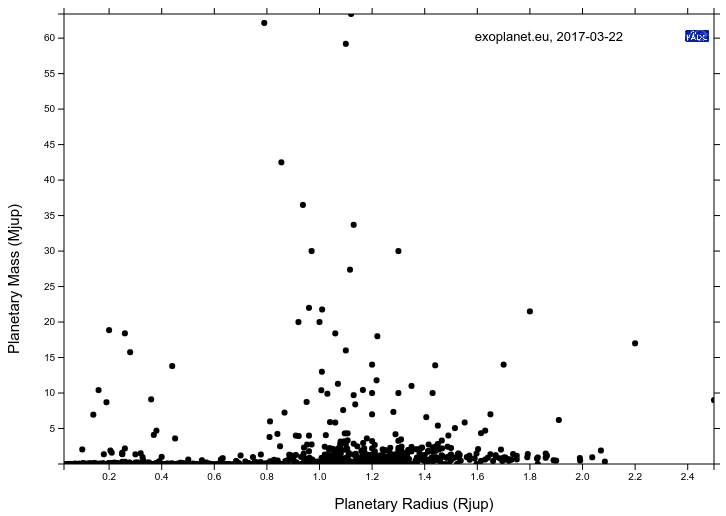
\includegraphics[width=0.80\textwidth]{exoplanets_MR_2.png}}
%\caption{Mass-radius relation for objects confirmed in planetary status\\ (on 22 Mar 2017), from \url{www.exoplanet.eu}}
%\label{fig_exbd}
%\end{figure}

%Conceptual discrimination between planets and brown dwarfs is based on a criterion involving an inobservable
%concept, namely its formation scenario, because we do not have the formation movie at hand. We can only rely
%on actual observables. Standard basic bulk observables are the object mass, radius, temperature. 
%An ideal situation would be that, at least for one of these observables, there
%are two domains $D_{p}$ and $D_{bd}$ of values which
%do not intersect. It is unfortunately not the case since there
%are planets smaller or larger, heavier or lighter, cooler or hotter than objects we believe to be brown dwarfs. 
%The choice made by the Extrasolar Encyclopaedia at exoplanet.eu, based on \cite{Hatzes2015}, is to take
%all objects below 60 Jupiter mass as planet.
%
%The \cite{Hatzes2015} argument is that the mass-radius and the mass-density relations presents no particular feature
%in the giant planet regime (i.e. more massive than Saturn) and that there is a change in the slope of distribution
%at 60 Jupiter mass (see Fig.\ref{fig_ajl2015}). 
%But unfortunately their statistics in the 30-60 Jupiter mass region is poor (the so-called desert) 
%since they rely only on transiting planets and do no consider the mass histogram in
%this region. Earlier data suggested a dip around 40 Jupiter mass \citep{Sahlmann2011, Udry2010} in the mass histogram. 
%More statistics will come in the near future, including radial velocity data from
%the ground and astrometric data from Gaia, to see if a feature around 40 Jupiter mass in the mass-radius diagram
%exists or not.
%
%\begin{figure}[!ht]
%\vspace{0cm}
%\centerline{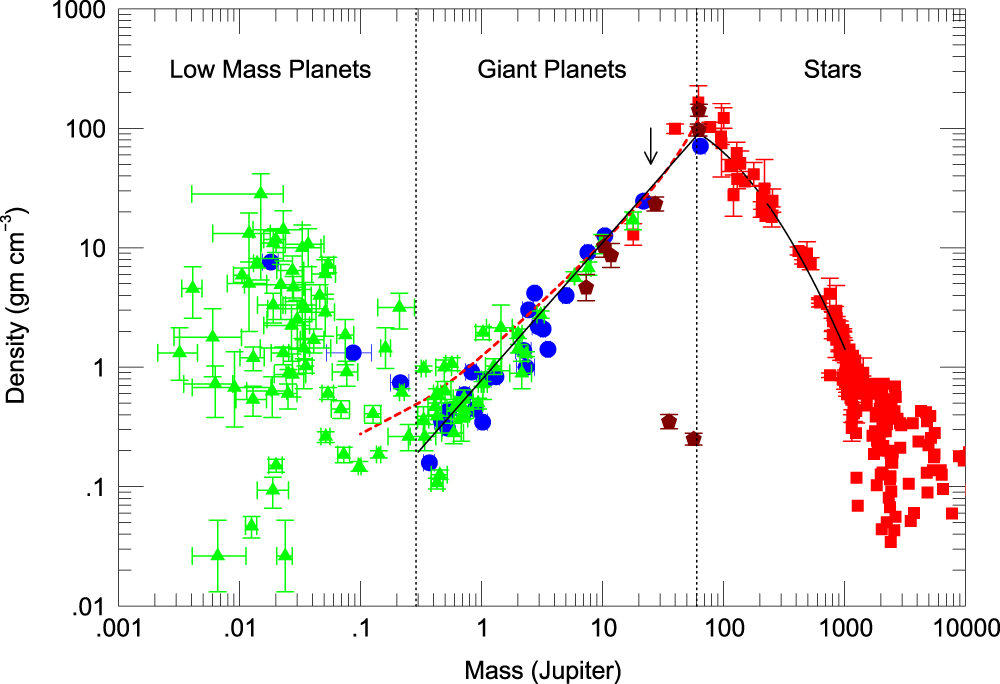
\includegraphics[width=0.80\textwidth]{apj2015.png}}
%\caption{Empirical mass-density relation. \textcopyright \cite{Hatzes2015}}
%\label{fig_ajl2015}
%\end{figure}
%
%A future improvement to separate the planet and brown dwarf populations will come from advanced observables,
%like the spectral type and species composition. They will help to constrain the formation mechanism of the object
%(accretion in a dust disk or collapse of a gas cloud).
%
%At least one conclusion is clear, the former mass limit of exoplanets at 13 Jupiter mass, corresponding to the triggering
%of nuclear burning of Deuterium, is not relevant since an object can be formed by dust accretion and acquire a
%final mass greater than 13 Jupiter.
%There is a second, more factual, problem: the value of observables can be very uncertain. This is especially the
%case for objects detected by imaging where the mass cannot be inferred from radial velocity measurements but only from
%spectra and models.
%The last problem, which we do not consider here because the concerned population is generally supposed to be small,
%is the “interstellar wanderers”, i.e. planets ejected by dynamical interaction from a well-formed planetary system.
%
%Assuming that the definition of a planet and a brown dwarf is adopted according to their formation mechanism, the separation 
%of the two populations is not an easy task \citep{COROT_book}.

\section{Common formation scenario: disk fragmentation}
\label{sect:formation_disk}

Disk fragmentation has been invoked both for the formation of brown dwarfs (BD) and giant planets (GP) and thus its pertinence must be examined as a general mechanism for the formation of sub stellar objects (SSO). 

The disk must be massive enough and fulfill the appropriate cooling conditions to become gravitationally unstable and lead eventually to the formation of GP or BD companions. 
Some simulations \citep{Stamatellos2007, Vorobyov2006} do predict BD formation at large orbital distances under such conditions, 
if the disk is massive and extended enough (typically $M_d\gtrsim 0.3\,\,M_\star$, $R_d\gtrsim 100\,(M_\star/ M_\odot)^{1/3}$ AU \citep{Stamatellos2009}). 
These simulations, however, lack a fundamental physical ingredient, namely the magnetic field. Indeed, it has been shown by several studies that magnetic fields prevent significant 
mass growth and stabilize the disk, severely hampering fragmentation \citep[e.g.][]{Hennebelle2008b,Price2009,Commercon2010,Machida2010}. 
Magnetic fields drive outflows and produce magnetic breaking, carrying out most of the angular momentum. 
These simulations, however, were conducted with ideal MHD. Subsequent calculations have shown that non-ideal MHD effects \citep[e.g.][]{Dapp2012,Machida2011b}, misalignment of the field with the rotation axis \citep{Hennebelle2009b,Joos2012,Li2013} 
and the turbulent nature of the velocity field \citep{Joos2013,Seifried2012,Seifried2013} all decrease the efficiency of magnetic braking. 
However, although large discs can form in these cases, they still remain smaller and less massive than the ones produced in pure 
hydrodynamical simulations. 
Three-dimensional calculations including radiation hydrodynamics, turbulence and complete MHD equations suggest that, for typical observed values of cloud magnetizations and rotation rates, large Keplerian disks do form during the initial core collapse phase
but do not seem to be massive enough to lead to fragmentation. 
This importance of magnetic field has received strong support from the confrontation of observations carried out at the PdBI with synthetic images derived from simulations of both pure hydro and MDH simulations \citep{Maury2010}. It was shown that the disk synthetic images derived from the MHD simulations were similar to the observed ones, with rather compact disks of typical FWHM $\sim 0.2^{''}$-0.6$^{''}$, while the hydrodynamical simulations were producing both too much extended disks and too fragmented (multiple) structures compared with observations. Moreover, observations of isolated disks at the early class 0 stage have revealed compact ($R\sim 20$ AU) disks \citep{Rodriguez2005}, 
while so far extended {\it massive} disks prone to fragmentation appear to be rare. Although better statistics is certainly needed to reach more robust conclusions.
Therefore, although disk fragmentation probably occurs in some disks at the early stages of star formation, 
the fragmentation process is largely overestimated in purely hydrodynamical simulations. Furthermore it is not clear
that fragments, if they form in the disk, will be able to cool quickly enough to form bound objects and to survive turbulent motions or rotational shear nor that they will not migrate quickly inward and end up been accreted by the star, leading to
episodic accretion events.

Other observational constraints seem to contradict gravitational instability (GI) in a disk as the {\it main route} for
BD or GP formation. If indeed this mechanism was dominant, most Class 0 objects should have massive disks, a conclusion which does not seem, 
so far, to be supported by observations. An argument sometimes raised by some proponents of this scenario \citep[e.g.][]{Stamatellos2009} is that the lifetime of the massive and extended disks produced in the simulations is too short ($\sim$ a few 10$^3$ yr) for the disks to be observed. This argument, however, does not hold since Class 0 objects last over a significantly longer period, about $\sim 10^5$ yr.
%, leaving statistically sufficient opportunities to see such massive disks.
Second of all, these simulations do not include an accreting envelope and thus end up too early compared with realistic situations, yielding an inaccurate diagnostic. 
As mentioned above, more accurate calculations including accreting envelope, magnetic field, turbulence and feedback (e.g. \citet{Seifried2013}; Masson et al., in prep.) show the emergence of large centrifugal disks but, for typical observed magnetic flux conditions, the disks do not appear to be massive enough to lead to fragmentation, at least for low mass protostars, the bulk of the
distribution. It is fair to say, however, that at the time these lines are written this important issue is far from being settled and further exploration of this topic is needed. As mentioned above, however,
it is mandatory to include all the proper physics in these studies to reach plausible conclusions. 

Most importantly, the observational constraints arising from the existence of wide BD or GP companions strongly argue against GI as an efficient formation mechanism. 
%An interesting exemple is the triple system LHS6343 \citep{Johnson2011}, with the presence of a BD companion with mass $M_C=0.063\, M_\odot$ to a low-mass star with $M_A=0.37\, M_\odot$. 
%Assuming disk-to-star standard mass fractions around $\sim 10\%$, the disk around $M_A$ should thus have a mass $M_d\approx 0.04\, M_\odot$. Although admittedly crude, this estimate shows that there is not enough mass in the disk to have formed the BD companion, even if assuming 100\% disk-to-BD mass conversion efficiency. 
Finally, the statistics arising from direct imaging revealing, at least so far, the scarcity of wide and massive SSO's in the BD or GP mass range around FGKM-type stars strongly argues against GI as the {\it main} formation mechanism for BD's or GP's. 
One might invoke the possibility that objects form by GI at large orbits and then migrate inwards closer to the star. 
This argument, however, does not hold. First, it must be stressed that
the possibility of migration is already included in the general analysis mentioned above. Secondly, if there was a "planetary" population forming by GI and migrating inwards, there should also be a "brown dwarf" population undergoing the same process. But this can be firmly observationally excluded. Finally, if we interpret the existing close-in planet population as objects that
formed by GI and migrated inwards, this would not explain planet bottom-heavy mass distribution and planet-metallicity correlation.
Gravitational instability, however, might occur in some particular situations, like for instance in very massive disks around {\it binary systems} \citep{Delorme2013}, even though other formation mechanisms are also possible in such situations.
The combination of ALMA and future direct imaging projects will definitely help nailing down this issue.

\section{Formation Scenarios For Brown Dwarfs}

\subsection{Photoionization}
The fact that the brown dwarfs (BD) mass function is about the same regardless of the presence or not of O stars shows that halting
of accretion by photoionizing radiation \citep{Whitworth2004} is clearly not a major mechanism for BD 
formation. Furthermore BD’s have been observed in isolated environments, excluding a necessary
connection between the presence of photoionizing radiation and BD formation.

\subsection {Accretion-ejection}
In the accretion-ejection scenario \citep{Reipurth2001}, BD’s are the result of accreting $\sim 1~M_{Jup}$ stellar
embryos, formed by the efficient dynamical fragmentation of a molecular clump, which get ejected from the surrounding 
gas reservoir and in the end remains in the sub-stellar domain. The characteristic conditions of this scenario are
(1) that dynamical interactions are responsible for the formation of both high-mass (by merging) and low-mass (by
ejection) objects, implying that star formation occurs basically, if not only, in dense cluster environments, 
(2) that the initial mass function (IMF) is determined essentially at the latest stages of the collapse, namely the ultimate gas-to-star conversion, with no correlation whatsever with the initial core mass function. 
In fact, pre-stellar cores do not really exist in this scenario.

The most achieved simulations exploring this scenario are made by \cite{Bate2012} which, although still
lacking magnetic field, include a treatment of gas heating and cooling. One of the most striking results of these 
simulations is that the resulting IMF reproduces quite well the \cite{Chabrier2005} IMF. These simulations, 
however, remain of questionable relevance for most Milky Way (MW) molecular cloud conditions. Indeed, it has been 
established observationally that star forming molecular clouds in the MW follow the so-called Larson’s relations \citep{Larson1981}, 
although with significant scatter, in terms of cloud size vs mean density and velocity dispersion 
(e.g. \citep{Hennebelle2012}): 
%$ \bar{n} \simeq 3 \times 10^3 \left( \frac{L}{1pc}\right)^{-\eta_d} ~cm^{-3} $,
%$\sigma_{rms} \simeq 0.8 \left( \frac{L}{1pc}\right)^{\eta} ~km~s^{-1}$ 
\begin{equation}
\bar{n} \simeq 3 \times 10^3 \left( \frac{L}{1~pc}\right)^{-\eta_d} ~cm^{-3}
\end{equation}

\begin{equation}
\sigma_{rms} \simeq 0.8 \left( \frac{L}{1~pc}\right)^{\eta} ~km~s^{-1}
\end{equation}
with $\eta_d \sim 0.7-1.0$ and $\eta \sim 0.4$.
Bate’s (2012) initial conditions, however, correspond to a 500 $M_{\odot}$ cloud at 10 K with size $L = 0.4~pc$, thus mean density 
$\bar{n} \simeq 3.2 \times 10^4 ~cm^{−3}$ and surface density $\Sigma \simeq 10^3 ~M_{\odot} ~pc^{−2}$ 
(while typcal values for MW molecular clouds are around $\sim 60-100 M_{\odot}~ pc^{−2}$ \citep{Heyer2009}). % and Mach number ${\cal M}=14$. 
These values correspond to rather extreme cloud
conditions, about 4 to 5 times denser and more turbulent than the aforementioned typical observed ones. Such conditions 
will support fragmentation and dynamical interactions and it is thus not surprising that they produce a
significant number of ejected BD embryos. Interestingly enough, these simulations can be directly confronted to 
observations. 
%Indeed, the simulated cloud mass and size are very similar to the ones of the young cluster NGC1333. 
%The simulations, however, produce a significantly larger number of stars+BD’s than the observed
%ones, with a total stellar mass $\sim 191\,M_\odot$ against $\sim 50\,M_\odot$ in NGC1333 \citep{Scholz2012a}; interestingly, this echos
%the aforementioned factors $\sim$ 4 in density and velocity.
Other inputs in the simulations, for instance the assumption of a uniform initial density profile, the lack of magnetic
field, and the underestimated radiative feedback all support fragmentation and thus probably overestimate the number
of proto-stellar or proto-BD embryos formed in a collapsing core, again supporting dynamical interactions/ejections. 
Observations in fact tend to suggest that fragmentation within pre-stellar cores is rather limited, most of the mass of the
core ending up in one or just a few smaller cores \citep{Bontemps2010, Tachihara2002}. This again
casts doubts on the relevance of such initial conditions to explore star/BD formation under typical Milky Way molecular 
cloud conditions. At least, if indeed BD formation by dynamical ejections might occur under some circumstances, 
existing simulations severely overestimate the efficiency of this process. In fact, one is entitled to suspect
that the similarity between the IMF produced by the simulations and the one representative of the Galactic field reflects
in reality the result of the initial gravoturbulent collapse of the cloud rather than the results of dynamical interactions.
In which case, the IMF in the simulations should already be largely determined at the begining of the simulation. If
this is the case, these simulations in fact bring support to star/BD formation by gravoturbulent collapse. At any rate,
until simulations with more realistic initial conditions are conducted, the ones performed by \cite{Bate2012} cannot be
considered as a reliable demonstration of dominant BD formation by accretion-ejection.

%The accretion-ejection scenario faces other important issues. Without being exhaustive, one can add a few more. (1)
%How can BD’s form, according to this scenario, in low-density environments? The Taurus cloud for instance, even
%though having a stellar density about 3 orders of magnitude smaller than other common clusters, has a comparable 
%abundance of BDs \citep{Luhman2012}. As noted by \cite{2011}, the low stellar density ($\lesssim 5~ stars /pc^2$ ) and
%low velocity dispersion of Taurus members ($\sigma \sim 0.2~ km~ s^{−1}$ ), indicate that there is no small N-body clusters from
%which stars or BDs could have been ejected, as advocated in the accretion-ejection scenario. The fact that BD’s form
%as efficiently in such low-density environments strongly argues against dynamical interactions. (2) Various observations 
%show average dispersion velocities of pre-stellar cores of about  $\langle \sigma \rangle \sim 0.4~ km~ s^{−1}$ \citep{Andr2009, Walsh2007, Muench2007, Gutermuth2009, Bressert2010}. This indicates a typical collision timescale 
%between pre-stellar cores significantly larger than their dynamical timescale, suggesting little dynamical evolution during
%pre-stellar core formation. (3) How can this scenario explain the observed similarity between the CMF and the IMF, if
%indeed such a similarity is confirmed?

All these observational constraints (notably the observed small velocity dispersion between protostar/BD’s) severely
argue against the accretion-ejection scenario for BD or star formation as a dominant mechanism, except possibly for
the most massive stars, which represent only a very small fraction of the stellar population.


\subsection{Gravoturbulent Fragmentation}
\label{sec:gravo}

In this scenario, large-scale turbulence injected at the cloud scale by various sources 
cascades to smaller scales by shocks and generates a field of density fluctuations down to the dissipative scale \citep[e.g.][]{MacLow2004}. Overdense regions inside which gravity overcomes all other sources of support collapse and form self-gravitating cores which isolate themselves from the surrounding medium. In this scenario, the mass function of pre-stellar cores (CMF) or IMF is set up by the spectrum of turbulence, at the very early stages of the star formation process. 
The first theory combining turbulence and gravity was proposed by \cite{Padoan2002} but has been shown to suffer from various warnings 
\citep[e.g.][]{McKee2007, Hennebelle2011a}. 
%Moreover, it requires the presence of a magnetic field to yield the proper IMF, in contrast to simulations. 
A different theory was derived more recently by \cite{Hennebelle2008a,Hennebelle2009a, Hennebelle2013} and \cite{Hopkins2012}. These latter theories nicely reproduce the IMF down to the least massive BDs, for appropriate conditions. The important feature
of these theories is that it is inappropriate to use the average thermal Jeans mass as an estimate of the characteristic mass for fragmentation. This would of course preclude significant BD formation. Indeed, in both Hennebelle-Chabrier and Hopkins theories, the spectrum of collapsing prestellar cores strongly depends on the Mach number, shifting the low-mass tail of the IMF to much smaller scales than naively expected from a purely gravitational Jeans argument. The theories indeed yield a reasonably accurate number of pre-BD cores for adequate molecular cloud like conditions and Mach values (${\cal M}\sim 3-8$). Densities required for the 
collapse of BD-mass cores, $\sim 10^7$-$10^8$ g cm$^{-3}$, are indeed produced by turbulence induced shock compression 
% (remembering that shock conditions imply density enhancements $\propto{\cal M}^2$). 
%Note that a similar scenario, taking into account the filamentary nature of the star forming dense regions, was developed by \cite{Inutsuka2001} (see chapter by {\it Andr\'e et al.}). 

Support for the gravoturbulent scenario arises from several observational facts. (1) It explains, within the framework of the same theory, the observed mass spectra of both {\it unbound} CO-clumps and {\it bound} prerestellar cores \citep{Hennebelle2008b}; (2) it implies that the IMF is already imprinted in the cloud conditions (mean density, temperature and Mach number), naturally explaining the resemblance of the CMF with the IMF; (3) it relies on one single "universal" parameter, namely the velocity power spectrum index of turbulence, which explains as well the Larson's relations for molecular clouds.

A major problem against the gravoturbulent scenario to explain the {\it final} IMF would arise if the cores were fragmentating significantly into smaller pieces during their collapse. Observations tend to show that
such fragmentation is rather limited. Numerical simulations of collapsing dense cores indeed show that radiative feedback and magnetic fields drastically reduce the fragmentation process \citep[e.g.][] {Krumholz2007, Offner2009, Commercon2010, Commercon2011, Hennebelle2011b,Seifried2013}. 
The analysis of simulations aimed at exploring the CMF-to-IMF conversion \citep{Smith2009} also show a clear correlation between the initial core masses and the final sink masses up to a few local freefall times \citep{Chabrier2010}, suggesting that, at least for the
bulk of the stellar mass spectrum, the initial prestellar cores do not fragment into many objects, as indeed suggested by the CMF/IMF similarity. But the most conclusive support for BD formation by gravoturbulent fragmentation comes from the emerging observations of isolated proto-BD's and of the pre-BD core Oph B-11\citep{Chabrier2014}.

\subsection{Formation of Binaries}
\label{bin_fn}

Newly formed stars must disperse a tremendous amount of angular momentum in condensing through more than 6 orders of magnitude in radius \citep{Bodenheimer1995}. Besides magnetic braking, binary formation offers a  convenient way
to redistribute at least part of this excess angular momentum. 

Several binaries have been observed at large {\it projected} separations ($>500$ AU) with masses down to $\sim 5\,M_{Jup}$. \cite{Looney2000} showed that multiple systems in the Class 0 and I phases are prevalent on large spatial scales ($\gtrsim$ 1000 AU) 
while binary systems at smaller scales ($\lesssim$ 500 AU) seem to be quite sparse \citep{Maury2010}.
Whether this lack of small scale binaries at the Class 0/I stages is real or stems from a lack of observations with sufficient resolution or sensitivity, however, is still unclear so far.
In any case, prestellar and protoplanetary disks do not extend out to thousand AU's so
formation of such wide BD binaries by disk gravitational instability (GI) seems to be clearly excluded. In contrast, such distances can be compared with the characteristic sizes of starless prestellar core envelopes, $\sim 10^4$ AU \citep{Menshchikov2010}. The existence of these wide systems thus suggests
that prestellar core fragmentation into binaries might occur at the very early stages of the collapse. Indeed, there are some observational evidences for binary fragmentation at this stage \citep{Looney2000,Duchene2003}. Moreover, the similarity, at least in a statistical sense, between some of the star and BD multiplicity properties suggests that most BD companions form similarly as stellar companions. This hypothesis has received theoretical 
and numerical support
form the recent work of \cite{Jumper2013}. These authors show that BD properties, including the BD desert, wide BD binaries and the tendency for low-mass (in particular BD) binaries to be more tightly bound than stellar binaries, arguments often used as an evidence for distinct formation mechanisms for BD's, can de adequately reproduced by angular momentum scaling during the collapse of turbulent clouds. 
Indeed, the early stages of cloud collapse/fragmentation and core formation are characterized by the formation of puffy disc-like structures which keep accreting material 
from the surrounding core envelope. These structures, however, are not relaxed and differ from structures purely supported by rotation, characteristic of relaxed, equilibrium discs.
Such "pseudo-discs" may fragment (as the result of global non-linear gravitational instability) during the (first or second) collapse of the prestellar core and end up forming (wide or tight) binaries, 
possibly of BD masses \citep{Bonnell1994, Machida2008}. 
The occurence of such fragmentation at the cloud collapse stage has been found in radiation-hydrodynamics simulations \citep{Commercon2010, Peters2011, Bate2012}. 
They remain to be explored in the context of resistive MHD before more definitive conclusions can be reached concerning this important issue. 
Such fragmentation into binaries occurs at the {\it very early stages of the core collapse}, during the main accretion phase. 
%They thus differ from the usual disk GI which involves a local, linear (Toomre) in a centrifugally supported disc. 
Whether it occurs dominantly by redistribution of angular momentum during the collapse itself or by global instability in the mass loaded growing pseudo-disk remains so far
 an open question and a clear-cut 
distinction between the two processes is rather blurry at this stage. 
It must be kept in mind, however, that the conditions for the formation {\it and} survival of bound fragments in a disk are subject to very restrictive constraints.


\section{Formation Scenarios For Giant Planets: Core \mbox{Accretion}}
\subsection{Core Accretion Mechanism}
In the core accretion scenario gas-giant planets form in two steps. First, a solid core is accumulated by accretion of
planetesimals. The growing core attracts a hydrostatic envelope of protoplanetary disk gas, extending from the 
surface out to the Bondi radius where the sound speed equals the escape speed of the core. Since accreting planetesimals
not only increase the core mass but also release gravitational energy, the energy released at the core surface must
be transported through the envelope, making the latter non-isothermal. The mass of the envelope increases with the
core mass faster than linearly, so that at some point the envelope starts to dominate the gravitational potential. 
Hydrostatic solutions cease to exist beyond a critical core mass which depends mainly on the accretion rate of solids and on
the gas opacity. As a result, core starts accreting mass on its own thermal timescale, turning itself into a giant planet.
\cite{Perri1974} assumed the hydrostatic envelope to be fully convective and found critical core masses
in excess of 100 Earth masses; they used this result to support the alternative gravitational instability scenario for
giant planet formation. \cite{Mizuno1980} allowed both for convective and radiative regions in the envelope and constructed 
the equilibrium model using gas opacities depending on the density and temperature, with a stepwise constant
dust opacity below the dust sublimation temperature. The radiative solution drastically reduces the critical core mass
to approximately 10 $M_\oplus$ , in agreement with constraints from the gravitational potentials of Jupiter and Saturn 
\citep{Guillot2005}, for an assumed mass accretion rate of $10^{−6} M_\oplus$ per year. Planetary envelopes can still be fully convective
at very high planetesimal accretion rates \citep{Wuchterl1993, Ikoma2001, Rafikov2006}, typical for cores at $\sim$AU
from the star, but this is unlikely to be an issue at large separations (Rafikov, 2006).
A generic property of the hydrostatic envelope is that its mass is inversely proportional to the luminosity (and hence
to the mass accretion rate) and to the opacity \citep{Stevenson1982}. The resulting critical core mass roughly scales as
$M_c \propto M^{1/4}$ \citep{Ikoma2000}. Hence the growth rate of the core partially determines the critical core mass. 
Beyond the critical core mass the envelope will emit more energy than provided by the gravitational potential release
of the accreted solids and undergo run-away contraction on the Kelvin-Helmholtz time-scale \citep{Bodenheimer1986}. 
Interestingly, the concept of a critical core mass seems to be supported observationally by the mass-radius
relationship of the recently detected Kepler low-mass transit planets \citep{Lissauer2011a, Lissauer2011b, Carter2012, Ofir2013}, 
bearing in mind the uncertainties in Kepler objects mass determinations. Indeed, while planets above
about $\sim 6 M_\oplus$ seem to have a radius requiring a substantial ($\gtrsim10$\% by mass) gaseous H/He envelope, so far planets 
below this mass have a radius consistent with a much lower, or even negligible gas mass fraction. 
%Even the rather extended
%gaseous envelope of the lowest transiting planet discovered so far, KOI-314c ($1.0^{+0.4}_{−0.3} M_{\oplus}$) (Kipping et al., 2014), 
%with a radius $R_{env} \sim 7^{+12}_{-13}$ \% of the planet’s radius, represents a negligible fraction ($\lesssim$ 3\%) of its mass.

\subsection{Time-scale for accumulation of the core}
In the classical core accretion scenario, the core grows by accreting planetesimals. The Hill radius
\begin{equation}
R_H = [G M_p /(3 \Omega^2 )]^{1/3} = 1/p R_p
\end{equation}
denotes the maximal distance over which the core can deflect planetesimals which pass by with the (linearized) Keplerian shear flow. 
Here $p = (9M_\star /4\pi \rho a^3 )^{1/3} \ll 1$ is a parameter that depends on semi-major axis $a$ and 
material density $\rho$ for a given stellar mass $M_\star$ (Goldreich et al.,2004). An additional random 
component to the particle motion will reduce the scattering cross section of the core to below $\sim R^2_H$.

The gravitational radius of the core denotes the maximum impact parameter at which a planetesimal approaching 
with velocity $v$ gets accreted by a core with radius $R$ at closest approach. This distance is given by
$R_G = R \sqrt{1+\frac{v^2_e}{v^2}}$
where $R$ is the radius of the core, $v_e$ the escape speed at the surface and $v$ the relative approach speed. In dynamically
cold discs planetesimals enter the Hill sphere of the core with the Hill speed $v_H = ΩR_H$ . In that case the gravitational 
radius can be simplified as $R_G \approx \sqrt{p R_H}$. 
A small fraction of the planetesimals which enter the Hill sphere of the core actually collide with it. 
The mass accretion rate is ultimately set by the gravitational radius and the
scale height of the planetesimals. The random motion of planetesimals enter both these quantities and should ideally
be calculated self-consistently using an N-body approach (\cite[e.g.][]{Levison2010}.

Assuming that the random particle motion is similar to $\Omega R_H$ — the Keplerian velocity shear across the Hill 
radius, one can find that the core grows at the rate \citep{Dones1993}
\begin{equation}
dR/dt\sim p^{-1}\Sigma_s\Omega/\rho\approx 50\,\,{\rm m\, yr}^{-1}(r/{\rm AU})^{-2},
\label{eq:drdt}
\end{equation}

Fragment accretion assuming surface density of solids typical for the minimum mass solar nebula (MMSN) ($\sim 30 g cm^{−2}$ at 1 AU). 
This corresponds to the mass growth rate of order $10^{−6} M_\oplus /year$ at 5 AU where Jupiter
presumably formed \citep{Dodson-Robinson2009}. This leads to core formation in $10^7$ years, in marginal agreement
with the observed life times of protoplanetary discs \citep{Haisch2001}, but the time-scale can be brought down by 
assuming a planetesimal column density that is 6-10 times the value in the MMSN (Pollack et al., 1996). Note that
eqn. (\ref{eq:drdt}) assumes uniform planetesimal surface density near the embryo, an assumption which may be violated if
the embryo is capable of clearing a gap in the planetesimal population around its orbit \citep{Tanaka1997, Rafikov2001, Rafikov2003a}, which would slow down its growth \citep{Rafikov2003b}. 

While the agreement between the core mass (or more exactly the total amount of heavy material) of Jupiter and 
the mass accretion rate necessary to form the core is a success
for the core accretion model, the mass accretion rate scales roughly as the semi major axis to the inverse second power
in accordance with equation (\ref{eq:drdt}). Hence core formation beyond 5 AU is impossible in the million-year time-scale of
the gaseous protoplanetary disc. This conflicts both with the high gas contents of Saturn, the small H/He envelope of
Uranus and Neptune and the observations of gas giant exoplanets in wide orbits beyond 10 AU \citep{Marois2008}.

This discussion makes it clear that gas giants can form by core accretion (CA) at large separations only if the core formation timescale
can be reduced dramatically. Ironically, acceleration of the core growth makes it harder to reach the threshold for CA,
because the critical core mass is inversely proportional to the core luminosity, which is predominantly derived from
the heat released in planetesimal accretion. Nevertheless, one can show \citep{Rafikov2011} that higher planetesimal 
accretion rate $\dot{M}$ still reduces the total time until CA sets in, even though the critical core mass is larger and is more 
difficult to achieve.

\subsection{Fragment Accretion}
One pathway to rapid core formation is to accrete planetesimal fragments damped by the gas to a scale height
lower than the gravitational accretion radius \citep{Rafikov2004}. 

Numerical and analytical studies of planetesimal dynamics generically find that soon after a dominant core emerges
it takes over dynamical stirring of the surrounding planetesimals, increasing their random velocities to high values.
Physical collisions between planetesimals then lead to their destruction rather than accretion, giving rise to a 
fragmentation cascade that extends to small sizes. \cite{Rafikov2004} demonstrated that random velocities of particles in a size
range 1 − 10 m are effectively damped by gas drag against excitation by the core gravity. Gas drag also does not allow
such small fragments to be captured in mean motion resonances with the embryo (\cite[e.g.][]{Levison2010}). This
velocity damping is especially effective in the vertical direction, allowing small debris to settle into a geometrically thin
disk with thickness below the maximum impact parameter, still resulting in planetesimal accretion ($\sim p^{1/2} R_H$). From
the accretion point of view the disk of such planetesimal debris is essentially two-dimensional, resulting in the highest
mass accretion rate possible in the absence of any external agents such as described in section \nameref{ss_pebble} below:
\begin{equation}
dR/dt\sim p^{-3/2}\Sigma_s\Omega/\rho\approx 1\,\,{\rm km\, yr}^{-1}(r/{\rm AU})^{-3/2}.
\end{equation}

This formula assumes that most of the surface density of solids $\sum_s$ ends up in small ($\sim$ 10 m) fragments dynamically
cooled by gas drag. Because of the dramatically reduced vertical scale height of the fragment population, this rate
is higher than the previously quoted (\ref{eq:drdt}) for the velocity dispersion $\sim  \Omega R_ H$ and decreases somewhat more slowly
with the distance (as $r^{−3/2}$ ). As a result, a Neptune size core can be formed at 30 AU within several Myrs.
A key ingredient of this scenario is the collisional grinding of planetesimals, which allows them to efficiently 
couple to gas and become dynamically cold, accelerating core growth. Fragmentation plays a role of an agent that transers 
mass from a dynamically hot mass reservoir 
%(population of large planetesimals, accreted at low rate because of relatively weak focussing) 
to dynamically cold debris. Even though at a given moment of time the latter population may
have lower surface density than the former, it is accreted at much higher efficiency and easily dominates core growth.
The importance of fragment accretion for accelerating core growth has been confirmed in recent coagulation simulations 
by \cite{Kenyon2009} (see also \cite{Levison2010}).
In the framework of this scenario \cite{Rafikov2011} sets a constraint on the distance from the star at which gas giants
can still form by CA in a given amount of time (several Myrs). By adopting the maximally efficient accretion of
small debris confined to a two-dimensional disk he showed that giant planet formation can be extended out to 40-50 AU
in the MMSN and possibly even further in a more massive planetesimal disk (out to 200 AU in the marginally gravitationally 
unstable gaseous protoplanetary disk). This estimate makes some rather optimistic assumptions such as
that most of planetesimal mass is in small (1-100 m) objects (e.g. as a result of efficient fragmentation), and that
seed protoplanetary embryos with sizes of at least several hundred km can be somehow produced far from the star
within several Myrs. Thus, it becomes very difficult to explain origin of planets beyond 100 AU by CA. This issue is
examined below.

\subsection{Pebble accretion}
\label{ss_pebble}

The arguably most fundamental particles to accrete are those forming directly by coagulation and condensation as
part of the planetesimal formation process. Several particle growth mechanisms predict that particles will stop growing
efficiently when they reach pebbles of millimeter and centimeter sizes.

While small dust grains grow as fluffy porous aggregates, they are eventually compactified by collisions around
mm sizes and enter a regime of bouncing rather than sticking \citep{Zsom2010}. This bouncing barrier maintains
a component of small pebbles which can feed a growing core. In the alternative mechanism where particles grow
mainly by ice condensation near evaporation fronts, particles sediment out of the gas when reaching pebble sizes.
This reduces their growth rate drastically as they must collectively compete for the water vapour in the thin mid-plane 
layer \citep{Ros2013}. Icy particles may be able to retain their fluffy structure against compactification
and hence avoid the bouncing barrier \citep{Wada2009}, but even under perfect sticking particles grow more slowly
with increasing mass and spend significant time as fluffy snow balls whose dynamics is similar to compact pebbles
\citep{Okuzumi2012}.

The dynamics of pebbles in the vicinity of a growing core is fundamentally different from the dynamics of a planetesimal 
or a planetesimal fragment. Pebbles are influenced by drag forces which act on a time-scale comparable to or
shorter than the orbital period, which is also the characteristic time-scale for the gravitational deflection of particles
passing the planet with the Keplerian shear. The gravity of the core pulls the pebbles out of their Keplerian orbits.
The resulting motion across gas streamlines leads to frictional dissipation of the kinetic energy of the particles and
subsequent accretion by the core. While planetesimals are only accreted from within the gravitational radius, which is
a small fraction of the Hill radius, pebbles are in fact accreted from the entire Hill sphere.

The potential of drag-assisted accretion was explored by \cite{Weidenschilling1985} who showed that particles 
below 1-10 meters in size experience strong enough friction to avoid getting trapped in mean motion resonances
with the growing core. \cite{Kary1993} confirmed these results but warned that only a small fraction (10-40\%) of the
drifting pebbles are accreted by the core due to their radial drift. This concern is based on the assumption that 
pebbles form once and are subsequently lost from the system by radial drift. This loss of solids would be in disagreement 
with observations of dust in discs of Myr age \citep{Brauer2007}. The solution to the drift problem may be that
pebbles are continuously formed and destroyed by coagulation/fragmentation and condensation/sublimation processes
\citep{Birnstiel2010, Ros2013}. Hence, any material that is not immediately accreted by the one or
more growing cores will get recycled into new pebbles that can then be accreted.

\cite{Johansen2010} simulated the accretion of small pebbles onto large planetesimals or protoplanets.
They found that pebbles with friction times less than the inverse orbital frequency are accreted from the entire Hill
sphere, in agreement with the picture of drag-assisted accretion. \cite{Ormel2010} interpreted the rapid 
accretion as a sedimentation of particles towards the core. \cite{Johansen2010} also observed that the pebbles
arrive at the protoplanet surface with positive angular momentum, measured relative to the angular momentum of the
disc, which leads to prograde rotation in agreement with the dominant rotation direction of the largest asteroids.

The dependence of the pebble accretion rate on the size of the core was parameterized in \cite{Lambrechts2012}. 
Below a transition core mass of around 0.01 Earth masses pebbles are blown past the core with the 
sub-Keplerian gas. Pebbles are captured from within the Bondi radius of the sub-Keplerian flow, which is much smaller
than the Hill radius. With increasing core mass the Bondi radius grows larger than the Hill radius, starting the regime
of efficient pebble accretion. Growth rates in this regime are 1,000 times higher than for accretion of large planetesimals
with velocity dispersion of order $\Omega R_H$ (see eqn. (\ref{eq:drdt})), at 5 AU, and 10,000 faster, at 50 AU, depending on the degree
of sedimentation of pebbles. Thus it is possible to make cores of 10 $M_\oplus$ even in the outer parts of protoplanetary
discs, which may explain observed gas giant exoplanets in wide orbits \citep{Marois2008}.

The accretion rate of pebbles depends on the (unknown) fraction of the solid mass in the disk which has grown to
pebble sizes. There is observational evidence for large pebble masses in some protoplanetary discs – the disc around
TW Hya should for example contain $0.001 M_{\odot}$ of approximately cm-sized pebbles to match the emission at cm 
wavelengths \citep{Wilner2005}. Such high pebble masses are surprising, given the efficiency for turning pebbles into
planetesimals via various mechanisms for particle concentration. However, if 
planetesimals form through streaming instabilities, then the simulations show that only around 50\% of the available pebble
mass is incorporated into planetesimals \citep{Johansen2012b}. The remaining pebbles are unable to concentrate
in the gas flow, due to their low mass loading in the gas, and are available for a subsequent stage of pebble accretion
onto the largest planetesimals.

The range of optimal particle sizes for pebble accretion falls significantly below the planetesimal fragments described 
above. Direct accretion is most efficient for particles which couple to the gas on time-scales from the inverse
Keplerian frequency down to 1\% of that value. That gives typical particle sizes in the range of cm-m in the formation
zone of Jupiter and mm-cm for planet formation in wide orbits, due to the lower gas density in the outer parts of 
proto-planetary discs. However, \cite{Morbidelli2012} showed that even boulders of 10 meters in size can be 
accreted with high efficiency, following a complex interaction with the core.

Although pebbles are not trapped in mean motion resonances, their motion is sensitive to the pressure profile of
the gas component. The global pressure gradient drives radial drift of pebbles towards the star, but any local pressure
maximum will trap pebbles and prevent their drift to the core. \cite{Paardekooper2006} showed that planets 
above approximately 15 $M_\oplus$ make a gap in the pebble distribution and shut off pebble accretion. The shut off is
explained in the analytical framework of \cite{Muto2009} as a competition between radial drift of particles and
the formation of a local gas pressure maximum at the outside of the planetary orbit. The core mass is already 
comparable to the inferred core masses of Jupiter and Saturn when the accretion of pebbles shuts down. \cite{Morbidelli2012} 
suggested that the termination of pebble accretion will in fact be the trigger of gravitational collapse of gas.

\subsection{Implications of rapid core accretion models}
In the pebble accretion scenario, cores of 10 $M_\odot$ or more can form at any
location in the protoplanetary disc, provided that a sufficient amount of material
is available. This can now be confronted with observational constraints from
exoplanet surveys. Direct imaging surveys now have good upper limits for the
occurrence rate of Jupiter-mass planet in wide orbits.
While many aspects of the observations and the luminosity of young planetary
objects are still unknown, it seems that gas-giant planets are rare beyond 25
AU (with $<23\%$ of FGKM stars hosting gas giants in such orbits). This can be
interpreted in three ways: 
(1) most of solids (pebbles, planetesimals) in protoplanetary discs reside in orbits within 20 AU, 
(2)
% there are not enough pebble-sized objects available for rapid core formation in wide orbits, 
wide orbits are mostly populated by ice giants as in the solar system, and 
(3)%(3) wide orbits are mostly populated by ice giants as in the solar system. 
gas-giant planets do form often in wide orbits but migrate quickly to the inner planetary system or are parts of 
systems which are unstable to planet-planet interactions shortly after their formation.
Regarding point (1), observations of protoplanetary discs in mm and cm wavelengths often find opacities that are consistent with large populations of pebbles \citep[e.g.][]{Wilner2005, Rodmann2006,Lommen2007}.
The fact that these pebbles are only partially aerodynamically coupled to the
gas flow, an important requirement for pebble accretion, was confirmed in the
observations of a pebble-filled vortex structure in the transitional disc
orbiting the star Oph IRS 48 \citep{vanderMarel2013}.

However, \cite{Perez2012} showed that particles are generally larger closer to the star, in
agreement with a picture where the outer regions of protoplanetary discs are drained of pebbles by radial drift. 
Regarding point (2), namely that wide orbits may be dominated by ice giants, it is an intriguing possibility, but its validation requires a
better understanding of why ice giants in our own solar system did not accrete massive gaseous envelopes.
Finally regarding point (3), it is important to keep in mind that massive planets in wide orbits have a
large gravitational influence which can lead to a disruption of the system. 
%The HR8799 system may owe its stability to a 4:2:1 resonance \citep{Fabrycky2010}, which indicates that a significant fraction of similar
%systems, less fortunately protected by resonances, may have been disrupted early on.

\subsection{Formation of the seeds}
Efficient accretion of pebbles from the entire Hill sphere requires cores that are already more massive than 0.1-1\%
of an Earth mass. Massive seed embryos are needed also in the rapid fragment accretion scenario \citep{Rafikov2011}. 
Below this transition mass pebbles are swept past the core with the sub-Keplerian wind. One can envision
three ways to make such large seeds: 
(1) direct formation of very large planetesimals, 
(2) run-away accretion of  plan-etesimals, 
(3) inefficient pebble accretion from large Ceres-size, the largest asteroid in the asteroid belt, planetesimals
to the transition mass.

Dust and ice grains grow initially by colliding and sticking to particle sizes which react to the surrounding gas flow
on an orbital time-scale. These pebbles and rocks, ranging from mm to m in size, experience strong concentration 
in the turbulent gas flow. Particles get trapped in vortices \citep{Barge1995, Klahr2003} and in large-scale pressure bumps which arise spontaneously in the turbulent gas flow \citep{Johansen2009b}.
Particles can also undergo concentration through streaming instabilities which occur in mid-plane layers of unity
dust-to-gas ratio, as overdense filaments of particles catch more and more particles drifting in from further out 
\citep{Youdin2005, Johansen2007a, Johansen2009a, Bai2010}. 
\cite{Youdin2005} performed a linear stability analysis of the equilibrium flow of gas and particles in the presence of a radial
pressure gradient. The free energy in the streaming motion of the two components - particles orbiting faster than
the gas and drifting inwards, pushing the gas outwards - forms the base of an unstable mode with growth rate 
depending on the particle friction time and on the local dust-to-gas ratio. Higher friction time and higher dust-to-gas 
ratio lead to shorter growth time. The growth time decreases by 1-2 orders of magnitude around a dust-to-gas ratio of
unity, which shows the importance of reaching this threshold mass-loading by sedimentation.

The streaming instability can concentrate particles up to several thousand times the local gas density in filamentary
structures \citep{Johansen2012a}. When particle densities reach the Roche density, the overdense filaments fragment
gravitationally into a number of bound clumps which contract to form planetesimals \citep{Johansen2007b, Johansen2009a,
Nesvorn2010}. The characteristic sizes of planetesimals formed by a gravitational instability of overdense 
regions seems to be similar to or smaller than the dwarf planet Ceres, the largest asteroid in the asteroid belt. Smaller 
planetesimals form as well, particularly in high-resolution simulations \citep{Johansen2012a}. However, for pebble 
accretion the largest planetesimal is the interesting one, since the accretion efficiency increases strongly with increasing
size. Nevertheless, a planetesimal with the mass of Ceres is still a factor 10 to 100 too light to undergo pebble 
accretion from the full Hill sphere. Hence suggestion (1) above, the direct formation of very massive planetesimals, is not
supported by the simulations. A more likely scenario is a combination of (2) and (3), i.e. that a large Ceres-mass
planetesimal grows by a factor 100 in mass by accreting other planetesimals through its gravitational cross section
and by accreting pebbles from the Bondi radius. This intermediate step between planetesimals and the seeds of the
cores could act as a bottleneck mechanism which prevents too many planetesimals from reaching the pebble accretion
stage. Hence only a small number of cores are formed from the largest and luckiest of the planetesimal population, in
agreement with the low number of giant planets in the solar system. The growth from 100-km-scale planetesimals
to 1000-km-scale planetary seeds, capable of rapid pebble accretion from the entire Hill sphere, has nevertheless not
been modelled in detail yet and represents an important priority for the future. The formation of a too high number
of competing cores could drastically reduce the efficiency of this growth path. 
\cite{Nesvorn2012} nevertheless argued for an initial number of no more than 10 growing cores which were subsequently 
reduced in number by collisions and ejections.


\section{Brown Dwarf or Giant Planet}
We can say that BD are like failed on the formation stage stars. 
Their masses are too small to permit the fusion of hydrogen in their nucleus. 
This characteristic allows to separate BDs from other stars based on their masses. 
So if star mass is below $0.07\ M_\odot$ for solar metallicity 
or $0.09\ M_\odot$ for lower metallicities \citep{Burrows2001} it is a BD 
or, in other words, we can say that star with a mass  $< 70\  M_{Jup}$ is a  
BD. 

It is more difficult to determining a lower mass limit for a BD. 
In practice, this limit can be defined as critical mass for the fusion of deuterium, which was defined by IAU in 2003 
as $\sim 10~M_{Jup}$ and later proposed around 13 $M_{Jup}$ in \cite{Bate2006},
but theoretically the lowest mass a BD could have may be just a few $M_{Jup}$ 
\citep{Larson1969,Silk1977,Boss1988}.
Good example of low mass BD is 
2M 1207 b \citep{Chauvin2005}, which is a $\sim 4~ M_{Jup}$ companion to a $\sim 20~ M_{Jup}$ brown dwarf. 
On the other side 13 $M_{Jup}$ is a typical for massive exoplanets, and, since there is no obvious upper-mass limit for an exoplanet, 
the problem of distinguishing between to two objects remains.

In \cite{Torres2016} authors make a large sample of well studied exoplanets and compare it with confirmed BDs available in the literature.
To compare the exoplanets with the BDs, authors combine the mass and radius 
into the baryonic gravitational potential (BGP) parameter, which is defined as the gravitational 
potential energy of a body, divided by the number of its nucleons, $N$. 
Assuming the mass is $M = N m_p$, where $m_p$ is the mass of a proton, the BGP is then equal to:
\begin{equation}
{\rm BGP} = \frac{V_G}{N} = \frac{G M m_p}{R} \propto \frac{M}{R}
\end{equation}
Since the BGP\ $ \propto M/R$, this parameter can be taken as 
a first order approximation for the mass-radius relations (MRR). 

\begin{figure}[!ht]
\centering
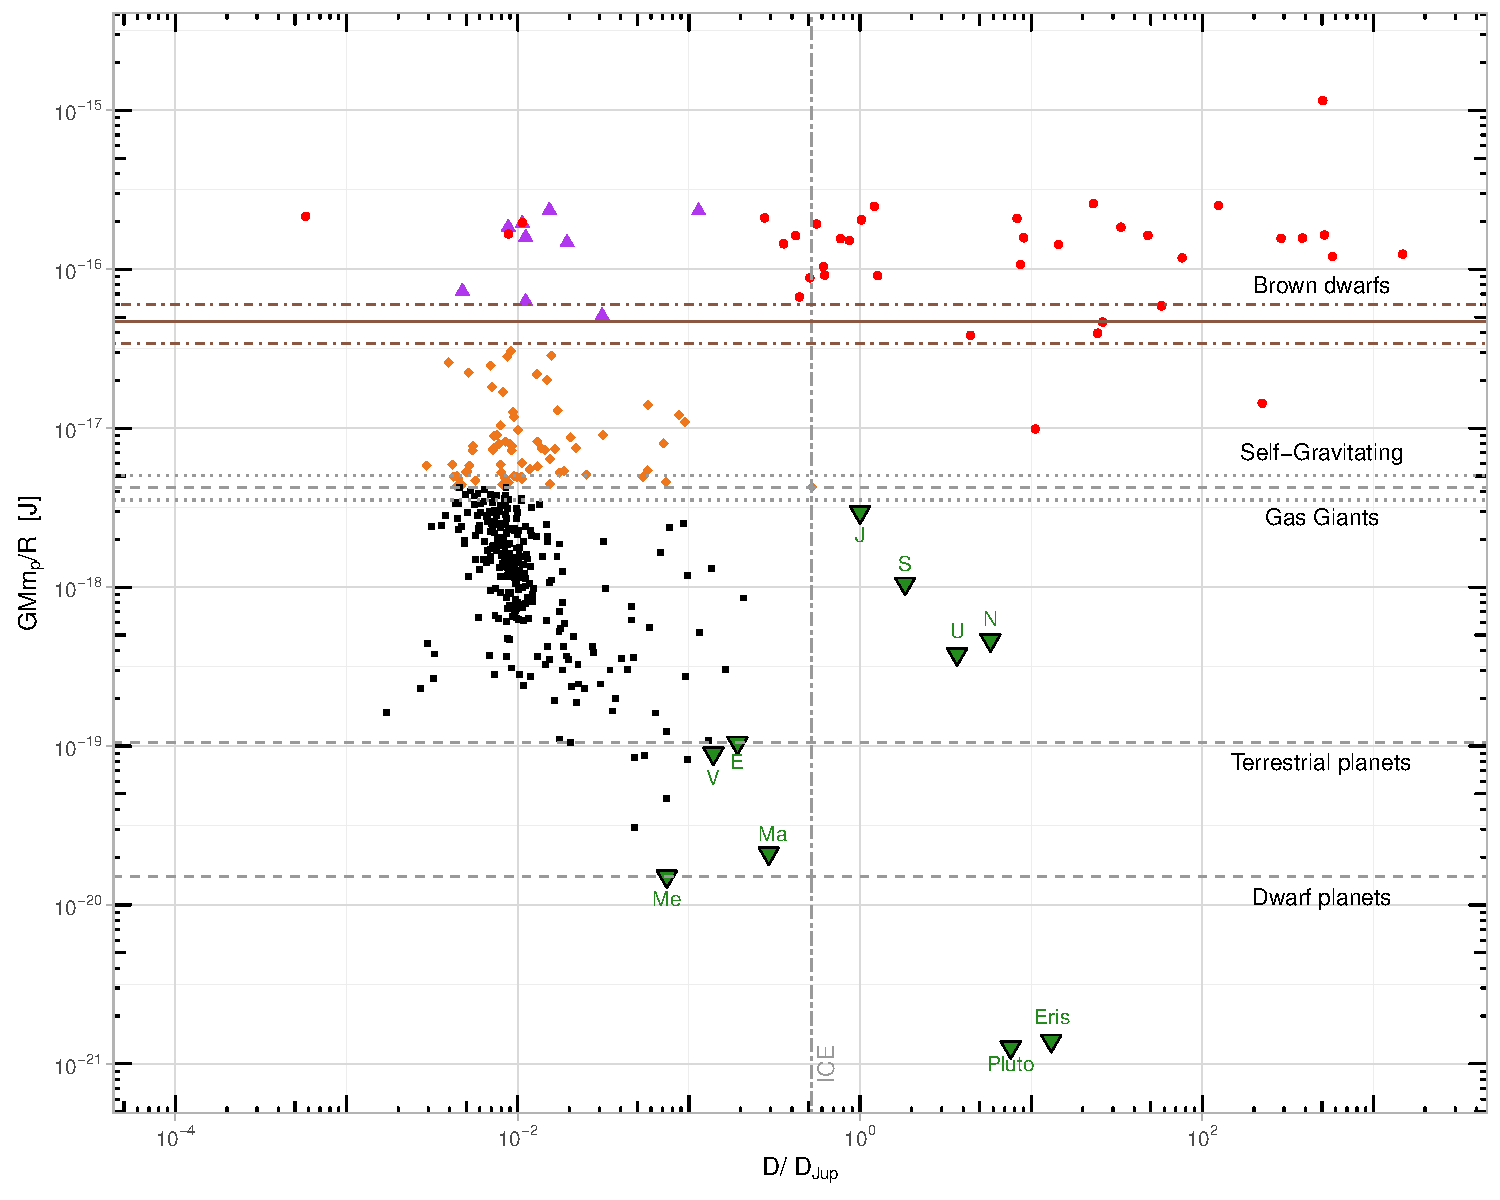
\includegraphics[width=0.85\linewidth]{f01.pdf}
\caption{The BGP diagram for exoplanets and BDs: nSGEs (black squares), SGEs (orange diamonds),  and BDs (red solid dots); the SGEs falling in BD region are identified by purple triangles. The inverted green triangles correspond to the positions occupied by the different kinds of planets in the solar system. The position of the ice line (or water "snowline") in the solar system (vertical dot-dash line) is also indicated. \citep{Torres2016}}
\label{fig:figTor1}
\end{figure}

In Figure~\ref{fig:figTor1} (hereafter, the BGP diagram) authors compare for the exoplanets (black squares and orange diamonds) and BDs (red solid dots) the BGP and distances from their companion stars, as normalized by the distance of Jupiter from the sun (${\rm D}/{\rm D_{Jup}}$). The BGP diagram is separated in four zones, synonymous with different physical structures. The upper zone is defined by the lower mass limit of $13\ M_{Jup}$ for the burning of deuterium in BDs. 

A few exoplanets are located above the deuterium-burning limit, while a few BDs are below this limit, suggesting that the deuterium-burning criterion does not allow a clear distinction between these two objects. Also, as observed by \citet{Santerne2016}, many BDs in this sample are found at a distance nearer than Jupiter from the Sun, that is in disagree with the BD's desert hypothesis. 
Therefore, although the majority of the exoplanets and BDs occupy different regions in the BGP diagram, their separation in terms of physical structures is still somewhat ambiguous.   

\begin{figure}[!ht]
\centering
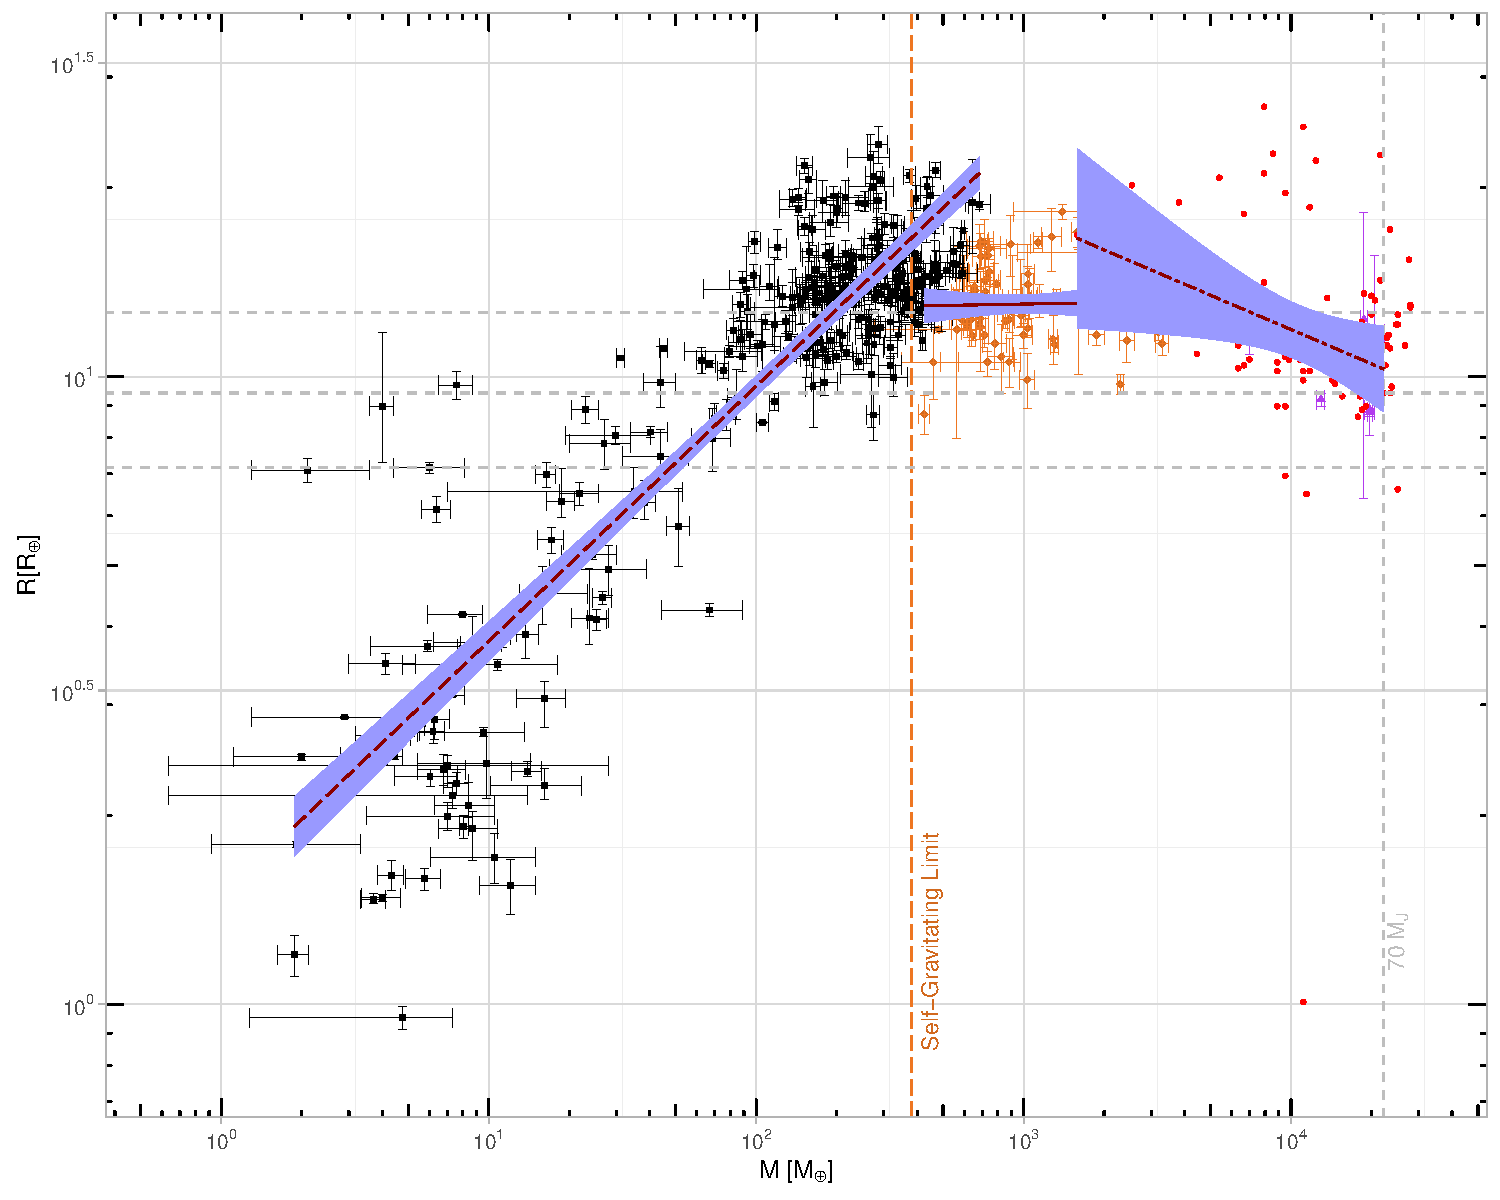
\includegraphics[width=0.85\linewidth]{f02.pdf}
\caption{Comparing the MRRs of exoplanets and BDs. The symbols are the same as in Fig. \ref{fig:figTor1}. Also shown are the critical mass at the SG limit and the upper mass limit $70~M_{Jup}$ for BDs.}\
\label{fig:figTor2}
\end{figure}

Based on the Self-Gravitating (SG) limit, separation on the gas-giant exoplanets in Self-Gravitating (SGE) and non Self-Gravitating (nSGE) was made.   
The BGP for the SG limit is defined by a critical mass, $M_c=1.2 M_{Jup}$, and critical radius, $R_c=0.84 R_{Jup}$ \citep{Padmanabhan1993}. 
Although both $M_c$ and $R_c$ are typical values 
for massive exoplanets, the critical mass is also comparable with the 
theoretical lowest mass expected for a BD, while the critical radius
is consistent with their observed mean radius \citep{Burgasser2008,Basri2006,Sorahana2013}.  

According to \citet{Padmanabhan1993}, the MRRs of 
bodies with different structures would be expected to change abruptly at the 
SG limit, from a positive MRR below the SG limit, to a negative one above it, which may help to separate exoplanets and BDs. 
This be observed on Figure~\ref{fig:figTor2}, where MRRs for the exoplanets and BDs are compared: the nSGEs show a positive MRR while the BDs show a negative one (see Table~\ref{tab:Tor1}). On the other hand, the SGEs show a relation where the radius does not increase with the mass. This characteristics was also observed by \citet{Hatzes2015}, although these authors did not offered any physical explanation for this behavior. 

\begin{table}[t]
\centering
\caption{Linear regression in log, $(R/R_{\oplus}) = 10^{b}\times (M/M_{\oplus})^a$, and their coefficients of correlation $r^2$.
Values from \cite{Torres2016}.}
\begin{tabular}{l c c c}
\noalign{\smallskip}\hline\hline\noalign{\smallskip}
\textbf{Sub-samples} & \textbf{a} & \textbf{b} & $r^2$\\
\noalign{\smallskip}\hline\noalign{\smallskip}
%SSP & $+0.29 \pm 0.01$ & $0.00 \pm 0.02$ & 0.995 \\
nSGE & $+0.41 \pm 0.01$ & $0.17 \pm 0.03$ & 0.785 \\
SGE & $+0.01 \pm 0.03$ & $1.09 \pm 0.10$ & 0.001 \\
BD & $-0.18 \pm 0.08$ & $1.60 \pm 0.33$ & 0.069 \\
\noalign{\smallskip}\hline
\end{tabular}
\label{tab:Tor1}
\end{table}

For the SGEs, we interpret the radius that shows no significant change as the mass increases as evidence for the presence of a dominant liquid metallic hydrogen (LMH) envelop \citep{Wigner1935,Hubbard1997,Dalladay-Simpson2016}: this is due to the very low compressibility of LMH \citep{Hubbard1997}. 

It was suspected by many authors that gas-giant planets, 
like Jupiter and Saturn in the solar system, have a LMH envelope \citep[see][and reference therein]{Burrows1993}. 
But, one would not expect to observe evidence for such envelopes. This is because, although the LMH layer could constitute 50\% to 85\% of the 
mass of a gas-giant planet, this layer would generally be hidden below a rich envelope of hydrogen gas. 
As the mass of a gas-giant exoplanet increased above the critical mass, $M_c$, the self-gravity of 
matter became more important, the pressure increased and most of 
the hydrogen in the outer gas envelope changed phase, transforming into LMH. 
Alternatively, since most of these exoplanets are Hot Jupiters with high eccentricities, they might have lost their outer envelop of gas when passing near their stars, revealing their underlying LMH envelopes \citep{Torres2016}. 

\begin{figure}[ht]
\centering
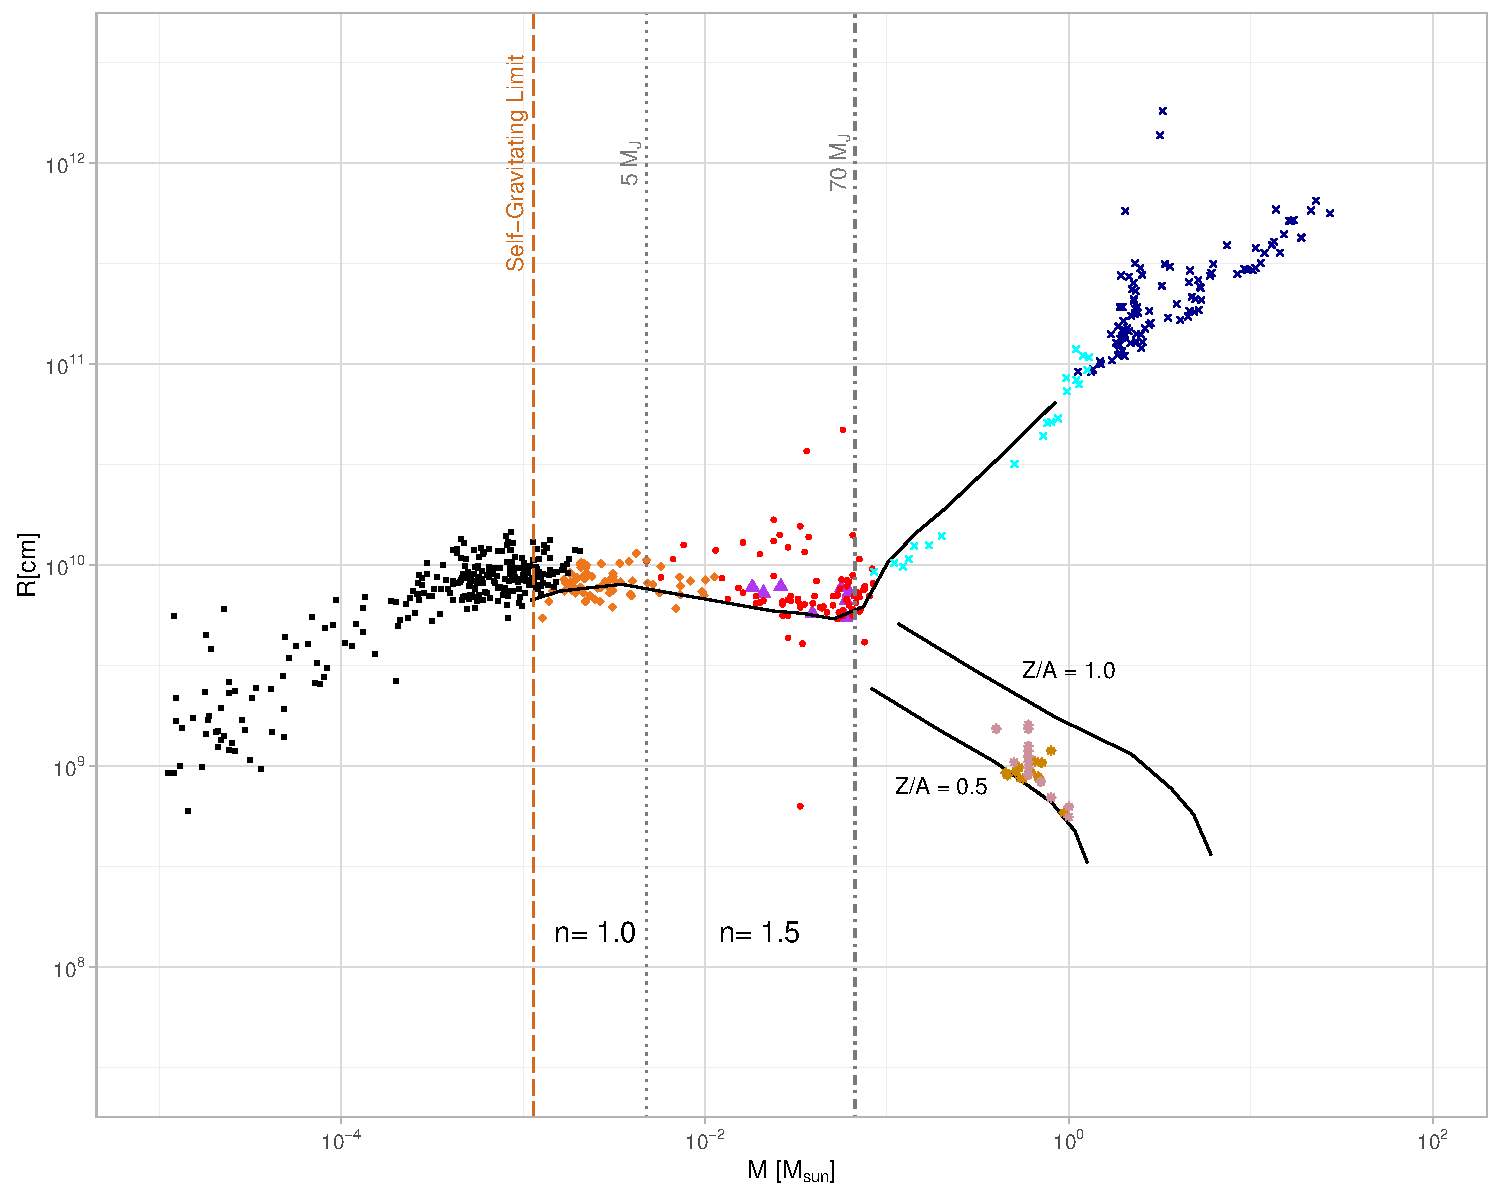
\includegraphics[width=0.85\linewidth]{f05.pdf}
\caption{Model of BDs formed of LMH. 
The MRR for the very low-mass stars (VLM, in light blue) becoming positive as they evolve towards the main sequence (dark blue x), 
while the MRR for WDs (white dwarfs, brown squares) is still negative. 
Two MRR for WDs, with different hydrogen richness (Z/A = 0.5 and Z/A = 1.0), are also represented. }
\label{fig:figTor3}
\end{figure}

However, based on the LMH interpretation there is still another alternative, which is that above the SG limit, objects are really BDs. In Figure~\ref{fig:figTor3} \citeauthor{Torres2016} compare their data with the predictions made by such a model, as developed by \citet{Burrows1993}. In this model BDs are formed at 99.9\% of 
LMH, this percentage decreasing as the mass of the star decreases, down to the SG limit. Below $5\ M_J$, the Coulomb correction competes 
with the degeneracy component, and the polytropic index, $n$, changes 
from 1.5 to 1.0, making the radius independent from the mass. 
According to this model, even above $5\ M_J$, 
when $n = 1.5$ and $R \propto M^{-1/3}$, the dependence of the radius on 
the mass would be weak, that corresponds to the low coefficients of correlation that was observed.  
According to this interpretation, therefore, it would be difficult, if not impossible, to distinguish between BDs and massive exoplanets. \citep{Torres2016}. 
While BD's appear to form preferentially like stars, from the graviturbulent fragmentation of a parent molecular clump, GP's form essentially by core accretion in a protoplanetary disk, i.e. from the grow of solids yielding eventually the accretion of a surrounding gas rich H/He envelope. So the definition of BD or GP is tightly linked with a processes of its formation mechanism.      
% % % % % % % % % % % % % % % % % %

\section{Detection of Exoplanets and Brown Dwarfs}
Several of the search methods for extrasolar planets and brown dwarfs are similar to those employed to
search for eclipsing and other periodic variable stars, but need to be more exact
because of the low amplitudes involved. At present, there is one direct and several indirect
methods available in the search for extrasolar planets which are discussed below.

\begin{itemize}
\item Direct (imaging/spectroscopy). In optical and infrared spectral regions, we can look for faint companions of
nearby stars, but true planets are not likely to be luminous enough to
be seen directly. It is even more difficult to obtain high spectral resolution 
to discern identifying features in the spectrum of any such candidate objects.
The difficulty is that the overwhelming light of the parent star makes it very difficult to
separate the flux of the planet from its star. Coronagraphic \citep{lyot1933}
and diffraction techniques are beginning to yield results as new generation space telescopes 
are an obvious answer to this need, but high resolution
techniques on existing telescopes may permit detection sooner \citep{milone2014}.

\item Astrometric variations.
Proper motions are secular angular motions in the plane of the sky, usually
expressed in units of arcsec/year in coordinates such as right ascension and declination.
They indicate slight changes in the direction of the star as seen from the Sun.
The size of this motion depends on the object's distance as well as the object's
linear motion across the line of sight. Periodic variation in the proper motion of
an object is a sign of binarity.
The method is applicable to any low-mass companions, and so to brown dwarfs
and planets as well as stars (astrometric binaries).

The amplitude of the variation depends on the ratio of the masses of the objects, which is inversely
proportional to the separation of the two objects from the centre of mass of the system.
If the mass of the system is known, for example, through a well-calibrated
mass-luminosity relation, the mass of the companion can be determined \citep{milone2014}.

\item Transits. While the radial velocity method provides information about a planet's mass, the photometric method can determine the planet's radius. This is the main advantage of the transit method. If a planet crosses (transits) in front of its host star's disk, then the observed visual brightness of the star drops by a small amount that depend on the relative sizes of the star and the planet. For example, in the case of HD 209458, the host star is dimmed by 1.7\%.

This method has two major disadvantages. First, planetary transits are only observable when the planet's orbit happens to be perfectly aligned from the astronomers vantage point. The probability of a planetary orbital plane being directly on the line-of-sight to a star is the ratio of the diameter of the star to the diameter of the orbit (in the case of small stars, the radius of the planet is also an important factor).
The second disadvantage of this method is a high rate of false detections. A 2012 study found that the rate of false positives for transits observed by the Kepler mission could be as high as 35\%-40\% in single-planet systems \citep{Santerne2012}. For this reason, a star with a single transit detection requires additional confirmation, typically from the radial-velocity method \cite{milone2014}.

\item Transit time variations.
Method for detecting exoplanets by observing variations in the timing of a transit. This provides an extremely sensitive method capable of detecting additional planets in the system with masses potentially as small as the Earth. In tightly packed planetary systems, the gravitational pull of the planets among themselves causes one planet to accelerate and another planet to decelerate along its orbit. The acceleration causes the orbital period of each planet to change. Detecting this effect by measuring the change is known as Transit Timing Variations.

\item Gravitational lensing. Unlike most other planet-detection techniques, gravitational microlensing
does not rely on detection of photons from either the host or the planet. Planets are discovered 
by their gravitational perturbation of light from a more distant source.

The most important attributes of the microlensing method are: (a) its sensitivity to planets orbiting
host stars with a broad range of masses located over a large range of Galactocentric distances;
(b) its sensitivity to low-mass planets, planets in wide orbits, free-floating planets, and, in particular,
planets with orbits at or beyond the so-called snow line (the location in the protoplanetary disk
where the disk midplane temperature is below the sublimation temperature of water); (c) the
fact that microlensing events and planetary perturbations are stochastic, rare, and unpredictable.

Microlensing detects planets through the instantaneous gravitational perturbation of the light
rays of a source star by the planet, as opposed to methods such as radial velocity or astrometry,
which require a full planet orbit to detect the gravitational influence of the planet on its host star.
Furthermore, when detected in conjunction with the microlensing event caused by its host star,
planets typically perturb light rays that pass close to the angular Einstein ring radius of the host
lens,
\begin{equation} \label{eq:ml_ring}
\theta_{E}\equiv \left( \dfrac{4GM}{D_{rel}c^{2}} \right) 
\end{equation}
where $M$ is the mass of the (host) lens, $D^{−1}_{rel} \equiv D^{−1}_{l} - D^{−1}_{s}$, and $D_{l},D_{s}$ 
are the distances to the lens and source \citep{gaudi2012}.

\item Radial velocity variations. 
A star with a planet will move in its own small orbit in response to the planet's gravity. This leads to variations in the speed with which the star moves toward or away from planet, i.e. the variations are in the radial velocity of the star with respect to planet. The radial velocity can be deduced from the displacement in the parent star's spectral lines due to the Doppler effect. The radial-velocity method measures these variations in order to confirm the presence of the planet using the binary mass function.

The speed of the star around the system's centre of mass is much smaller than that of the planet, because the radius of its orbit around the centre of mass is so small. However, velocity variations down to 1 m/s or even somewhat less can be detected with modern spectrometers, such as the HARPS spectrometer at the ESO 3.6 meter telescope in La Silla Observatory, Chile, or the HIRES spectrometer at the Keck telescopes.

Until 2014, the radial-velocity method was by far the most productive technique used by planet hunters. It is also known as Doppler spectroscopy. The method is distance independent, but requires high signal-to-noise ratios to achieve high precision, to find lower-mass planets. This method easily finds massive planets that are close to stars. Modern spectrographs can also easily detect Jupiter-mass planets orbiting 10 astronomical units away from the parent star, but detection of those planets requires many years of observation.

Planets with orbits highly inclined to the line of sight from Earth produce smaller visible wobbles, and are thus more difficult to detect. 
One of the advantages of the radial velocity method is that eccentricity of the planet's orbit can be measured directly. One of the main disadvantages of the radial-velocity method is that it can only estimate a planet's minimum mass.

\item Indirect effects on (O-C) diagrams of EBs.
Times of minimum light from EB constitute a time stamp on the system. If there is a planet in circumbinary orbit around the binary stars, the stars
will be offset around a binary-planet centre of mass. As the stars in the binary are displaced back and forth by the planet, the times of the
eclipse minima will vary. 
The periodicity of this offset may be the most reliable way to detect extrasolar planets around 
close binary systems \citep{deeg2000, doyle1998}. With this method, planets are more easily detectable 
if they are more massive, orbit relatively closely around the system, and if the stars have low masses.

The eclipsing timing method allows the detection of planets further away from the host star than the transit method. 
%However, signals around cataclysmic variable stars hinting for planets tend to match with unstable orbits \citep{horner2013}. 
In 2011, Kepler-16b became the first planet
to be definitely characterized via eclipsing binary timing variations \citep{doyle2011}.

Proto-planetary disks have been seen around several stars, including $\beta$ Pictoris
and Vega, and remnants of disks have been seen around older stars. Gaps and
warping have been attributed to the presence of planets or proto-planets in some of
these systems \cite{milone2014}.
\end{itemize}



% Chapter 2
\chapter{Eclipsing Binaries and Their Period Changes} % Main chapter title
\label{ch:EB} % For referencing the chapter elsewhere, use \ref{Chapter1} 

%----------------------------------------------------------------------------------------
% Define some commands to keep the formatting separated from the content 
\newcommand{\keyword}[1]{\textbf{#1}}
\newcommand{\tabhead}[1]{\textbf{#1}}
\newcommand{\code}[1]{\texttt{#1}}
\newcommand{\file}[1]{\texttt{\bfseries#1}}
\newcommand{\option}[1]{\texttt{\itshape#1}}
%----------------------------------------------------------------------------------------

Eclipsing binaries are periodic variable stars (the cycle of variation repeats relatively reliably). 
This broad group was historically divided into three phenomenological
classes according to the appearance of the light curves: Algols, $\beta$ Lyrae systems, and W Ursae Majoris systems.
 
On the other side, morphological classification based on the Roche equipotentials provide more physical insight. Associated with the
concept of equipotentials are “limiting surfaces” or “limiting lobes.” A limiting
lobe is the volume enclosed by a limiting surface. The usefulness of morphological
classifications is that each of the stable configurations is generated by a structural-evolutionary process.

There is some correspondence between the morphological classification based on
the Roche lobes and the phenomenological classification (see section \ref{EB_classif}):
\begin{center}
Algol-type light curves $\Rightarrow$ detached and semi-detached systems\\
W UMa-type light curves $\Rightarrow$ over-contact systems.\\
\end{center}

Phenomenological classification of the $\beta$ Lyrae-type light curve has
no morphological counterpart. Sometimes, $\beta$ Lyrae-type light curves are produced
by detached systems, sometimes by semi-detached systems, and sometimes also by
systems having marginal over-contact. However, there are semi-detached binaries that are not
Algols (e.g., cataclysmic variables) and over-contact binaries that are not W UMa’s.

The characteristics of EB types according to morphological classification will be
discussed in the following section.


\section{Eclipsing Binaries Systems Classification}
\label{EB_classif}
The dynamic forces controlling the stellar mass distributions involve the effects of
rotation, tides, and non-circular orbits. For an introductory-level discussion of all
these effects, see \cite{wilson1974}. Fortunately, tidal forces produce circular orbits and
synchronous rotation in many interacting binaries. A detailed and excellent analysis
of the tidal evolution in close binary systems is provided by \cite{hut1981}. The orbital
period of a synchronous rotator in a circular orbit is the same as the rotation period.
We will discuss only synchronous rotation.

Another physical simplification reduces the mathematical complexity: although
the stars may be relatively large and considerably distorted, they attract one another
nearly as if their entire masses were concentrated into mass points at their centres. 
Therefore, only two forces need to be considered in the circular orbit and
synchronous rotation case: (i) gravitational attractions of two mass points;
(ii) the centrifugal force due to the rotation of the entire binary system about its centre of mass.
These two forces produce gravitational potential, which can be written in the form:
\begin{equation} \label{eq:roche_pot}  % Zasov "Obshchaja astrophys" p.212
\Omega_{R} = \dfrac{2}{(1+q)(r_{1}/a)}+\dfrac{2}{(1+q)(r_{2}/a)} + \dfrac{(x-\mu a)^{2}+y^{2}}{a^{2}}
\end{equation}
where\\ 
$q = M_{1}/M_{2}$,\\ 
$a=a_{1}+a_{2}$, \\
$r_{1}= \sqrt{x^{2}+y^{2}+z^{2}}$ ~and~ $r_{2}= \sqrt{(x-a)^{2}+y^{2}+z^{2}}$, \\
$\mu = M_{2}/(M_{1}+M_{2})$ \\

Given that both gravitational and centrifugal forces are time-wise constant for co-rotating 
matter, we can expect to find solutions for static configurations in the co-rotating frame. 
A somewhat similar problem was solved by the French mathematician Roche (1820--1883) in the nineteenth century. 
The basic concept for understanding the solutions of that problem is equipotential surfaces
(briefly, equipotentials). These are surfaces on which the sum of rotational and
gravitational energy per unit mass is constant. On these level surfaces, also called
\textquote{Roche surfaces}, the component of the force vector tangential to these surfaces vanishes, i.e., 
the local force vector is everywhere normal to them. The Roche surfaces
are indeed the static surfaces we are interested in: they co-rotate with the orbital
motion of the binary. Binary component surfaces are now modelled as equipotentials
(similarly on Earth, where ocean and lake surfaces follow equipotentials).

If one of the stars slowly expands, due to evolution, it will eventually fill its
Roche lobe. If the star expands further, the \textquote{path of least resistance} for the expanding matter
is through the inner Lagrangian point -- called $L_{1}$ -- into the Roche lobe of the
other star; the Roche lobe will overflow. The material falls toward the other star,
but, since it is carrying angular momentum, it falls in a spiral pattern.
There are five Lagrangian points, labelled $L_{1}$ to $L_{5}$, all in the orbital plane of the two main bodies. The first three are on the line connecting the two main bodies.
The last two, $L_{4}$ and $L_{5}$, each form an equilateral triangle with the two main bodies. The two latter points are stable, which implies that objects can orbit around them in a rotating coordinate system tied to the two main bodies \citep{Percy2007}.

The degree of star and Roche lobe contact is measured by the contact parameter, $f$ , sometimes
called the fill-out factor:
\begin{equation}
f = \dfrac{\Omega^{I}-\Omega}{\Omega^{I}-\Omega^{O}}, ~~~ \Omega^{I}\leq \Omega^{O}
\end{equation}
where $\Omega^{I}$ and $\Omega^{O}$ are modified potentials at the inner and outer Lagrangian surfaces respectively. 
%In a system of two orbiting stars, the gravitational potential energy is constant on the surfaces.
%Close to each star, the surfaces are almost spherical. But there is a \textquote{critical}
%surface -- the one which is hour-glass shaped (or figure-eight shaped, for those not familiar with hour-glasses, though, 
%as noted below, the surfaces are three-dimensional like an hour-glass, not two-dimensional like a figure eight). 
%The two halves of the hour-glass are called Roche lobes. The point of intersection
%of the hour-glasses is the inner Lagrangian point.
%https://ru.wikipedia.org/wiki/%D0%9F%D0%BE%D0%BB%D0%BE%D1%81%D1%82%D1%8C_%D0%A0%D0%BE%D1%88%D0%B0
%https://ru.wikipedia.org/wiki/%D0%A2%D0%BE%D1%87%D0%BA%D0%B8_%D0%9B%D0%B0%D0%B3%D1%80%D0%B0%D0%BD%D0%B6%D0%B0
%https://en.wikipedia.org/wiki/Lagrangian_point

According to Roche lobe fill by its star eclipsing binaries are classified to:
\begin{enumerate}
\item \textbf{detached systems} (Fig.\ref{fig:eb_det}), if neither component fills its Roche lobe.
The fill-out factor of each component is negative. If the components are small compared with their 
Roche lobes, their shapes closely approximate spheres. Whereas morphology and evolutionary state are related 
for semi-detached and over-contact binaries, such a connection does not exist in detached systems;
\item \textbf{semi-detached systems} (Fig.\ref{fig:eb_semidet}), %if one component fills its Roche lobe, and the other does not;
with one component within its critical lobe, whereas the other exactly fills its lobe ($f = 0$ for this component). This morphological
type includes Algols, cataclysmic variables, and some X-ray binaries, in which
one component is highly evolved and in which mass transfer occurs. In general, the lobe-filling star can
lose matter through the inner Lagrangian point;
\item \textbf{over-contact systems} (Fig.\ref{fig:eb_overcont}) %, if both components exceed their Roche lobes.
or common envelope binaries, where each component has
a surface larger than its Roche lobe. Mechanical equilibrium requires that the sur-
faces match in potential. That is, the common surface must coincide with a single
equipotential above the Roche lobes ($0 < f_{1,2} \leq 1$,~and~$f_{1} = f_{2}$). Configurations
are limited by the outer Lagrangian surface. This morphological type explains W UMa stars very well \citep{kallrath2009eclipsing}. %p107, 112
\end{enumerate}

\begin{figure}[!t]
\vspace{0cm}
\centerline{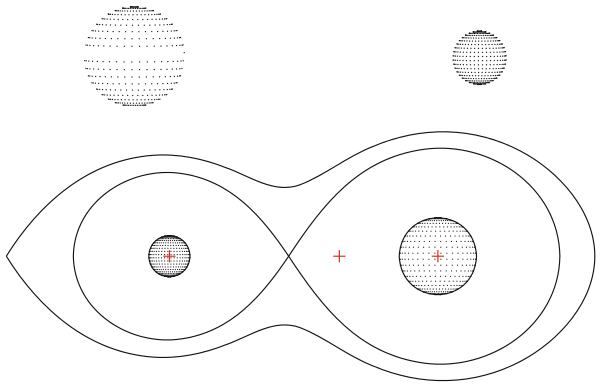
\includegraphics[width=0.56\textwidth]{EB_detached.png}}
\caption{Roche potential and shape of a detached binary system. The plot has been produced using Binary Maker 3.0 and 
the YZ Cassiopeia parameter set provided in the examples collection \citep{bradstreet2005}.($f_{1}<0, f_{2} < 0$)}
\label{fig:eb_det}
\end{figure}
\begin{figure}[!t]
\vspace{0cm}
\centerline{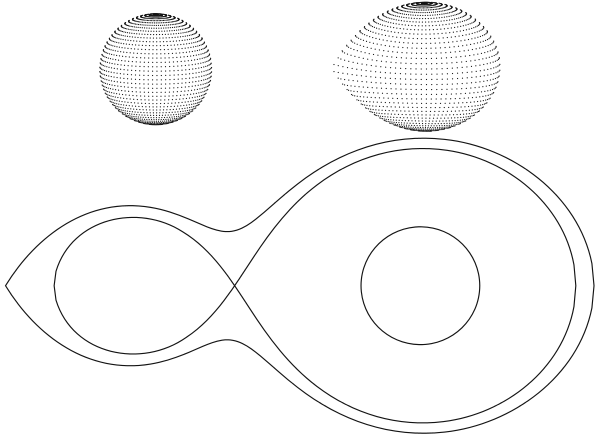
\includegraphics[width=0.56\textwidth]{EB_semidet.png}}
\caption{Roche potential and shape of a semi-detached binary. The plot has been produced with
Binary Maker 2.0 using the Algol parameter set in the examples collection \citep{bradstreet1993}. The primary component fills its Roche lobe 
($f_{1} = 0, f_{2} < 0$)}
\label{fig:eb_semidet}
\end{figure}
\begin{figure}[!t]
\vspace{0cm}
\centerline{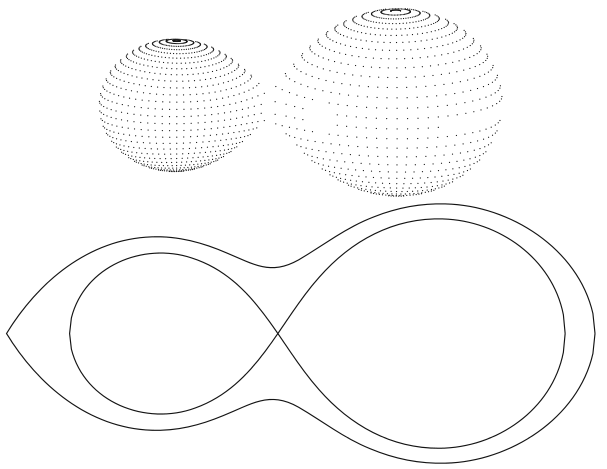
\includegraphics[width=0.56\textwidth]{EB_overcont.png}}
\caption{Roche potential and shape of an over-contact binary. The plot has been produced with
Binary Maker 2.0 for the TY Bootis parameter set in the examples collection \citep{bradstreet1993}.
Both components exceed their Roche lobes. ($0<f_{1,2}\leq1, f_{2} =f_{1}$)}
\label{fig:eb_overcont}
\end{figure}

%\section{Why Binary Stars Are Important}
\section{The Importance of Binary Stars}
Binary stars are important, first, because they are numerous. \cite{latham1992} 
conclude that the frequency of spectroscopic binaries detected in the galactic
halo is not significantly different from that in the disk, despite differences in
kinematic properties and chemical composition. The observed frequency is approximately
20\%; the actual frequency is higher because many binaries remain undetected.
In the solar neighborhood, where we have the benefit of proximity so that
proper motion variations can be detected, the frequency is more than 50\% -- and
several stars are in fact multiple systems.
The second reason why binaries are important is that they are the primary source
of our knowledge of the fundamental properties of stars. For example, the direct
determination of the mass of any astronomical object requires measurable gravitational
interaction between at least two objects (galaxy-galaxy, star-star, star-planet,
planet-satellite). In galaxy-galaxy interactions, the distances and separations are
so large that no detectable motion on the plane of the sky is possible. In star-planet
interactions, the objects contrast so greatly in brightness that outside the solar system
only the highest possible precision can resolve the objects. 
Typically in the latter case, only the star's motions are detectable, and the
properties of that star must be assumed, mainly on the basis of binary star studies, in
order to deduce the properties of the planet. In star-star interactions, the variations
in position and velocity caused by orbital motion are detectable for a wide range
of stellar separations and up to at least a factor of 5 in brightness. It is often the
case that both stars may be studied in any of several ways, depending on their distances,
brightnesses, and motions. Other basic properties of stars and of the systems
they constitute can be determined through analysis of observational data, depending
on the observational technique by which the interaction is studied \citep{kallrath2009eclipsing}. 

The full determination of absolute eclipsing binary parameters requires both a
light curve and a radial-velocity curve for each component. EBs are informative
objects because they allow photometry and spectroscopy to be combined effectively.
Eclipsing, double-lined systems are rare but very valuable. If the data quality is high
and the binary configuration is well conditioned, we have a fundamental source of
information about sizes, masses, luminosities, and distances or parallaxes of stars.
Many other parameters can be determined from precise light curve data if the configuration 
fulfills certain requirements, for example, by having complete eclipses.
Because such stars may be found over the full range of ages, they also tell how stars
evolve -- at least in binary stars \citep{kallrath2009eclipsing}.


\section{EB Systems Period Change}
\label{ch:EB_p}
Period changes in binary systems are generally due to one of three
mechanisms.
\begin{enumerate}[label=(\roman*)]
\item A loss of angular momentum from the system, or mass transfer.

\item The presence of a third body in a long orbit around the binary.
This affects the light traveltime, which can be misinterpreted as
a change in the binary period. For example, as the binary moves
towards the observer, the eclipses are seen to occur more frequently
than when the binary is moving away.

\item Applegate’s (1992) mechanism, where period changes are
caused by coupling between the binary period and changes in the
shape of the secondary star.
\end{enumerate}

% % %mass transfer
The most frequently mentioned explanation for period changes
in close binary systems is the transfer of mass from one star to another.
In \cite{Nanouris2011} authors present a equation \ref{eq:orb_angm} that reveals a close connection between the orbital angular momentum and the period of the system. Non-conservative
mass loss mechanisms increase the orbital period, while angular momentum loss processes, such as magnetic breaking and gravitational
radiation, lead to a period reduction.

\begin{equation}
\label{eq:orb_angm}
J_{orb} = \frac{M_1 M_2 G^{2/3}}{(2\pi)^{1/3}(M_1+M_2)^{1/3}}P^{1/3}
\end{equation}

From \cite{Tran2013} relation between mass transfer and amplitude of O-C modulations can be represented as:
\begin{equation}
\frac{\dot{M}}{M} \approx 4\pi^2 \frac{Amp}{T^2} 
\end{equation}
where $Amp$ and $T$ are rough measures of the amplitude and cycle time of the wave in the O-C curve.

%The most frequently mentioned explanation for period changes
%in close binary systems is the transfer of mass from one star to another. 
%However, mass transfer from a less massive to a more massive component results in a steadily increasing
%period not an alternating sequence of period increases and decreases. Mass transfer also appears to be an unsuitable
%explanation for the cyclic O-C pattern seen in close binaries for another reason. 
%The RS CVn systems, in which cyclic O-C patterns are present, are in general detached systems (Hall 1976), 
%so mass transfer cannot be invoked.
%Mass loss due to stellar winds also appears to be ruled out.
%DeCampli \& Baliunas (1979) have shown that, for RS CVn stars, the mass-loss rates required to produce a quasi-periodic signal in 
%the O-C diagram are orders of magnitude larger than allowed by observations. 
%They note that such losses would conflict with the detection of soft X-rays from
%$\alfa$ Aur, UX Ari, HR 1099, and RS CVn. 
%If we assume a single process produces the cyclic O-C curves, neither of these processes appear to be viable.
%
%
%The period change can also be explained by angular momentum loss from the binary system. Angular momentum loss is governed by two mechanisms -- gravitational radiation and magnetic braking. 
%The rates of angular momentum loss caused by both mechanisms must be added together to find the total angular momentum loss for the
%system. 
%
%The expression for gravitational radiation is given by \cite{Brinkworth2006}:
%\begin{equation}
%\left( \frac{dJ}{dt} \right)_{grav}=-\frac{32}{5} \frac{G^{7/2}}{c^5}a^{-7/2}M_1^2 M_2^2 M^{1/2}
%\end{equation}
%where $M_1$, $M_2$ and $M$ are the primary mass, secondary mass
%and total mass, respectively, and $a$ is the binary separation given
%by Newton’s form of Kepler’s third law $a = (G M/ω^2)^{1/3}$
%
%The standard model for magnetic braking in CVs is based upon
%studies of the solar wind and the rotation periods of solar-type stars
%in open clusters (Weber \& Davis 1967; Skumanich 1972; Mestel \&
%Spruit 1987). Rappaport et al. (1983) developed an empirical prescription that is still commonly used in CV studies. This relationship
%is given by
%\begin{equation}
%\left( \frac{dJ}{dt} \right)_{mb}=-3.8 \times 10^{30} M_\odot R_\odot^4 m_2 r_2^\gamma \omega^3 ~erg
%\end{equation}
%where $0\leq \gamma \leq 4$ is a dimensionless parameter and $\omega$ is the angular
%frequency of rotation of secondary star in $rad~s^{−1}$.

% % % 3 body
Apparent changes in the orbital periods of binary stars have often been attributed to the light travel time variation caused by third
bodies although further observation usually reveals that this cannot be the case.
Changes in eclipse timings of binary stars do not necessarily
indicate a genuine change in the binary period. 
A third body in a long orbit around the binary can cause small but significant changes in the
light travel time from the binary system, which manifest themselves
as strictly sinusoidal changes in the timings of mid-eclipse \cite{Brinkworth2006}.
Amplitude of light travel time variation caused by third
body than can be expressed as:
\begin{equation}
K = \frac{M_3 G^{1/3}}{c} \left[\frac{P_3}{2\pi(M_1+M_2)} \right]^{2/3}
\end{equation}
where $M_3$ is a mass of third body; $P_3$ - period of third body; $M_1, M_2$ - massses of primary and secondary components of EB system;  $G$ - gravitational constant; $c$ - speed of light (see \cite{Pribula2012} for details).

% % %Applgate
Quasi-periodic variations in eclipse times over timescales of years to decades in the orbital periods of 
eclipsing binary stars is known as the Applegate effect \cite{Applegate1992}. 
This mechanism invokes magnetic activity cycles in the low-mass components of such
binaries to redistribute angular momentum within the interior of the star, thereby changing the stellar quadrupole moment which leads to changes in the orbital period of the components. Later, \cite{Lanza1998} proposed
that the Applegate mechanism could also be driven by effectively converting rotational kinetic energy and magnetic
energy back and forth. Regardless of the details of the exact physical mechanism at work, the Applegate effect should
also operate in most exoplanet systems since the host stars are (by selection) low-mass stars with a convective outer
layer which should exhibit some form of dynamo activity \cite{Watson2010}.
%It will therefore be important to know the magnitude of the Applegate effect for exoplanet systems when interpreting any TTVs. 
According to Applegate mechanism, solar-like magnetic cycles would result in shape
changes of the low-mass components, thus redistributing the angular momentum within
the interior of the star. Then, the oblateness is changed, causing a change of the stellar
quadrupole moment which consequently leads to the variation of orbital period. 
The amplitude of orbital period modulation and the amplitude of
the oscillation in the O-C diagram are related by equation
\begin{equation}
\frac{\Delta P}{P} =2\pi \frac{A}{P_{mod}}
\end{equation}
where $A$ and $P_{mod}$ are the amplitude and modulation period of the cyclic oscillation
of the orbital period, and $\frac{\Delta P}{P}$ - period change.
% % % % % % % % % % % % % % % % % % % % % % %

%Several hypotheses have been advanced to explain the cyclic period changes in close binaries. Apsidal motion,
%which involves a change in the orientation of the binary’s major axis, is an unlikely mechanism because close binaries
%possess circular orbits, and this phenomenon only occurs in systems having large eccentricities. 
%If apsidal motion were present, the times for secondary and primary minima would be shifted in opposite directions, 
%but this effect is rarely seen and does not appear to be present in Algols. 
%An alternate possibility is that the cyclic pattern in the O-C plot is
%caused by the presence of a third body. This idea has been explored by several investigators, most recently by Borkovits \& Hegedu¨s (1996). These researchers postulate that the motion of the binary around the center of mass of a triple
%system causes the primary and secondary eclipse times to vary in a uniform and periodic fashion. In this case, the
%cyclic O-C pattern arises from orbital-induced changes in the distance to the observer. 
%Finally, Hall (1989) noted that, for Algols that possess alternating period increases and decreases, the spectral types of 
%the secondaries are always in the range late F to K. 
%These stars have outer convective zones and, if they are rapidly rotating, a magnetic dynamo
%is produced (Parker 1979). Applegate (1992) and Lanza, Rodono`, \& Rosner (1998) used this information to develop
%a theory to explain the cyclic shape of the O-C curves of these systems. They suggest that if the secondary is
%deformed by tidal and centrifugal forces, changes in the internal rotation associated with a magnetic activity cycle
%alter the star’s gravitational quadrupole moment. As the quadrupole moment increases the gravitational field
%increases, leading to a decrease in the binary period. Conversely, when the quadrupole moment decreases, the binary
%period increases (Lanza \& Rodono` 1999).
\chapter{Motivation}

According to outlined above in section \ref{ch:EB_p}, one of the reasons of eclipsing binary system period change is a light time travel effect or presence of $3^{rd}$ in EB system. That's why I decide to investigate existence of brawn dwarfs and circumbinary planets in eclipsing binary systems.

In next sections of my PhD thesis I will briefly describe O-C diagram tool as a instrument for detection of period changes in EB systems. 
I will investigate all factors that has a influence on O-C diagram shape, and thus affect on determination of orbital parameters of brawn dwarfs and circumbinary planets that can exist in EB system.
These factors are -- EB system visibility from observational point, weather conditions, precision of photometry, presents of spots on EB component, or on both components, pulsations in eclipsing binaries.

something more ... simulation  $10^6$   


Using all described above knowledge distortion presented on O-C diagrams of eclipsing binary systems I will try to search brawn dwarfs and circumbinary planets in eclipsing binary systems using Kepler eclipsing binaries catalogue or from ground based observations.  

\chapter{O-C Diagrams and Simulations}
\label{ch:oc_sim}

In this chapter we briefly describe O-C diagrams as a method that we use for 
detection of $3^{rd}$ bodies (circumbinary planets or brawn dwarfs in our case) in eclipsing binary systems.
Also we present our simulation of $3^{rd}$ bodies in eclipsing binary systems.

\section{O-C Diagrams}
Observed minus Calculated diagrams is a diagnostic tool and interpretation 
of the disagreement between the measure of an observable event and its predicted value \citep{Sterken2005basic}.
In astronomy, O-C diagram usually is used when discussing cyclic phenomena where the times of occurrence of a given event is irregular. 
The O-C diagram is then constructed by plotting the quantity O-C as a function of time, the correct interpretation 
of these deviations leads to a better model (and a new O-C diagram).

In variable-star studies, O-C is sometimes expressed as deviations of phase
in the cycle of variability, whereas the time axis is the cycle number (commonly indicated by $E$). 
In such studies, the O-C diagram mostly refers to rather simple C formalisms, viz. linear or quadratic ephemeris formulae, sometimes
combined with a trigonometric periodic term \citep{Sterken2005basic}.

During the building O-C diagram we are dealing with processes that repeat themselves in a more or less regular way.
Any attempt to construct a reliable O-C diagram will fail if a wrong value of period $P$ is used. 
But it is not always easy to derive a period from the observational data: 
$P$ is not directly observable, it follows from the
determination of at least two moments of time of the same reference phase (epochs). 
The observation of two such epochs $T_{1}$ and $T_{2}$ immediately provide us an upper limit for $P$. 
When more than two such times are available, the period can be derived by a least-squares solution of a set of
equations
\begin{equation} \label{eq:period}
T_{i} - T_{j} = nP
\end{equation}
where $n$ is an integer, commonly called the cycle number $E$(epoch).

Phase is a position on the cycle of variation, a convenient periodic measure of
elapsed time: $\varphi (t)$ is the fraction of $P$ that elapsed since the occurrence of the
reference time $T_{0}$ and is given by

\begin{equation} \label{eq:phase}
\varphi = \frac{T-T_{0}}{P} ~\bmod~ 1
\end{equation}

The most common approach to the O-C procedure is the one in which one reference 
phase is selected, and where the timings of this reference phase are studied
and interpreted.


If $P$ is constant and if its value is known, equation (\ref{eq:period}) leads to

\begin{equation} \label{eq:Tmin2}
T_{min} = T_{0} + P E
\end{equation}

where $T_{min}$ is the time of minimum light, $T_{0}$
is the zero epoch and $E$ is the number of cycles elapsed since the zero epoch. $T_{0}$ and
$P$ are obtained through a least-squares solution. The longer the time interval (in
cycles) over which the data have been collected, the higher will be the accuracy
of the solution for $P$: the uncertainty in $P$ is inversionally proportional to the
number of cycles, and proportional to the r.m.s. scatter of the data.

It is hard to conclude from experimental data that a period change has occurred. 
In principle, changes of period could be described by any mathematical formula expressing $P$ as a function of time.
Thus, the time of epoch $T_{m}$ is

\begin{equation} \label{eq:P_var}
T_{m} = T_{0} + \int P(t)dt   ~~~~~\mathrm{or}~~~~~   T_{m} = T_{0} + \int P(E)dE
\end{equation}

In most cases, relation (\ref{eq:P_var}) is restricted to linear variations, cyclic variations, or
a combination of both of them.

Many causes can lead to period variations.
Transfer of matter (between stars in a multiple system) or mass ejection (from a system)
can provoke period changes. And what is most important for our research - periodic variations of O-C can indicate presents of other body in binary system.

After construction of O-C diagram there can be a visible trend present on the residual diagram.
Such a trend, in particular when it repeats itself, 
can indicate presence of other body in binary system. 
In such case, O-C can be fitted with additional term corresponding to 3rd body orbit parameters:  

\begin{equation} \label{eq:P_lin_OC_sin}
T_{m} = T_{0} + P_{0}E + \frac{1}{2} \frac{dP}{dt} \bar{P}E^{2} +
\dfrac{a_{12}\sin i}{c}   \left[  \dfrac{1-e^2}{1+e \cos\nu}   \sin(\nu + \omega)  + e \sin \omega  \right]
\end{equation} 

where $a_{12} \sin i$ is the projected semi-major axis, $e$ is the eccentricity,
$\omega$ is the longitude of the periastron, $\nu$ is the true anomaly of the EB orbit around the common centre of the mass of
the whole system and $c$ is the velocity of light \citep{irwin1952}.

\section{Determination of Minima Times}
\label{sec:methods}
To make O-C diagram we have to determine time of minima of eclipsing binary system. We need to define function that will fit minima shape with best precision.
There is a two different approaches that can be made an the beginning of precise time of minima determination. First - to fit complete light curve, and second - to fit only minima parts. In my research I will use the second approach, also I will prefer to use simple function fitting, because there is no big difference in precision of minima determination with other methods described below and we have a large number of eclipses in our simulations so time of calculation is also important factor. 


\subsection{Kwee and van Woerden Method}
Method is based on assumption that the set of data points around the minimum can be represented by the curve that is strictly 
symmetric with respect to the true minimum epoch $T_{0}$. Then an even function of time $\tau=T-T_{0}$ can be chosen to
fit the observations in sense of least-squares method. However the function itself is not evaluated. Instead a preliminary 
minimum time $T_{1}$ is estimated and $2K$ magnitudes (equation \ref{eq:kwee_m}) spaced at equal time intervals $\Delta$ symmetrically to $T_{1}$ are formed by linear interpolation between the observations.  Then $S(T_{1})$ is computed.
\begin{equation} \label{eq:kwee_m}
m_{\pm k} = m(T_{1}\pm k \Delta), ~~~ k=(1,K)
\end{equation}

\begin{equation} \label{eq:kwee_S}
S(T_{1}) = \sum_{k=1}^{K}(m_{k}-m_{-k})^2
\end{equation}

The procedure is repeated twice by shifting assumed minimum time by~ $\pm \Delta/2$ ~yielding $S(T_{1}+\Delta/2)$ ~and~ $S(T_{1}-\Delta/2)$.
The three values of $S$ define a parabola~ $S(T)=aT^2+bT+c$ ~with minimum at~ $T_{KW}=-b/2a$ ~which is considered to represent the 
true minimum time $T_{0}$. The mean error of minimum epoch is estimated by

\begin{equation} \label{eq:kwee_err}
\sigma_{KW} =\sqrt{\frac{4ac-b^2}{4a^2(Z-1)}} 
\end{equation}
where $Z$ is the number of independent magnitude pairs. For~ $2K=N$  ($N$ is a number of observations) the authors take  $Z=N/4$ ~if observations are not equally spaced in time ~\citep{kwee1956, brainhorst1973}.

Main disadvantage of this method is that we must have symmetrical shape of minimum and error of such method are unrealistically small. 

%\subsection{Simple Function Methods}

\subsection{Fitting with Gauss, Lorentzian and Moffat Functions}
The main advantage of this functions is their simplicity and ability to get coordinates of centre ($x_{c}$) after fitting light curve.
With another more complex functions that are discussed below we must to derivate it before we can find $x_{c}$.

Gaussian function:
\begin{equation}\label{eq:gaus}
F(t)= A\cdot \exp(-\frac{(t - x_{c})^2}{2\sigma^2})
\end{equation}

Lorentzian function: 
\begin{equation}\label{eq:lorentz}
F(t)= A \frac{w^2}{w^2 + (t - x_{c})^2}
\end{equation}

Moffat function: 
\begin{equation}\label{eq:moffat}
F(t)=  A \left( 1 + \frac{(t - x_c)^2}{\sigma^2} \right)^\beta      % (\frac{1 + (t - x_c)^2}{g^2})^{-k}
\end{equation}
where $A$ is the amplitude, $t$ is the time, $w$ is the half-width at half-maximum, $\sigma$ is the standard deviation and $x_{c}$ is the coordinates of centre. 

Functions perform good fit when EB minima has shape similar to normal distribution. In case of narrow minima such functions have a slightly larger error. Of course, function perform good fit only when we fit only minima part but not all light curve.

\subsection{Fitting with Polynomial Function}
Polynomial function is fitted to light curve in a time interval $2 \Delta t$, symmetric with respect
to the estimated minima time. The times of minima are then found using 
the calculated first derivatives, and the resulting list is processed again in
subsequent iterations. Two choices must be carefully made:
\begin{enumerate}
\item The optimal value of $\Delta t$: evidently, $\Delta t$ should comprise only those data
that contribute to the minimum event being considered, and should exclude 
data beyond the flection point. The time interval $\Delta t$ should by all
means be sufficiently large to avoid small-number statistics, and the fitted
parameters must be reasonably stable when omitting data points near the
edges of the interval $2 \Delta t$
\item The degree of the polynomial: parabolic fits are to be avoided, since they
force symmetry to the data. Polynomials of third degree work well if data
curves have a slight asymmetry, but for more extreme skewness, fourth- or
fifth-degree polynomials may be used. The order of the polynomial should
be appropriate in relation to the number of data points: though the formal
goodness of fit may appear to increase with increasing polynomial degree,
one should avoid high orders when dealing with sparse data.
\end{enumerate}

The choices are very much dictated by the data, perhaps most of all by the
observational precision, and by the time resolution.
The safest approach, probably, is to carry out a statistical investigation with a range of $\Delta t$ and polynomial
degrees 3-5 for every reference phase of every variable studied, and to select the
best-fit combination of reference phase, interval and polynomial degree for that
particular variable.

But the solution really depends on the chosen interval
and on the number of data, we should keep in mind the rule of thumb that the order
of the polynome should respect the number of fitted points \citep{Sterken2005basic}.

\subsection{Phenomenological Methods}
\label{phenom}
Different methods of non physical LC fitting exists, 
main goal of such methods is to define function that will fit desired type of LC with good accuracy. 
Below we describe two most popular phenomenological methods.
  
First method is proposed in work \cite{mikulasek2015} and aimed to establish a general model of LCs of eclipsing binaries that could fit the LCs with an accuracy of 1\% of their amplitudes or better. Method also works for stars with transiting planets.

The model function of a monochromatic light curve of eclipsing
systems $F(\varphi, \lambda)$, can be assumed as the sum of three particular functions:

\begin{equation} \label{eq:mik_general}
F(\varphi, \lambda) = F_{e}(\varphi, \lambda) + F_{p}(\varphi, \lambda) + F_{c}(\varphi, \lambda)
\end{equation}
where $F_{e}$ describes the mutual eclipses of the components, $F_{p}$ models the proximity effects,
while $F_{c}$ approximates the O'Connell effect (irrespectively of its physical cause).

%The profiles of both minima are complex functions determined primarily by the geometry
%of the system and the relative brightness of components. 

The model function was selected by \cite{mikulasek2015} to describes as aptly
as possible those parts of LCs that are in the vicinity of their inflex points, where their slopes are maximum. 
The functions are parameterized by their widths $D_{1}, D_{2}$, eclipse LC kurtosis
coefficients $\Gamma_{1}, \Gamma_{2}$, dimensionless correcting factors $C_{1},C_{2}$, and
central depths $A_{1}(\lambda_{eff}), A_{2}(\lambda_{eff})$:

\begin{equation} \label{eq:mik_main}
F_{e}(\vartheta, \lambda_{eff})=\sum_{k=1}^{n_{e}} A_{k} \left( 1+C_{k} \frac{\varphi_{k}^2}{D_{k}^2}\right) 
\left\lbrace 1-\left\lbrace 
1-\exp\left[ 1-\cosh\left(\frac{\varphi_{k}}{D_{k}}\right)\right] 
\right\rbrace^{\Gamma_{k}}\right\rbrace 
\end{equation}

\begin{equation} \label{eq:mik_2}
\varphi_{k} = \vartheta - 0.5 (k - 1) - \mathrm{round} \left[ \vartheta - 0.5 (k - 1)\right] ,
\end{equation}
where $\vartheta$ is a phase function, the summation is over the number of eclipses during one
cycle, $n_{e}$: $n_{e} = 2$ or $n_{e} = 1$ (the common situation for exoplanet
transits). Each eclipse in a given colour is thus described by only
four parameters -- its depth $A$, width $D$, kurtosis $\Gamma$, and the correcting
parameter $C$.

In the case of EBs with two minima in a cycle ($n_{e} = 2$), we
need eight parameters, but sometimes the number of needed parameters
can be smaller. 
Inspecting the parameters $D, \Gamma$, and $C$ for both eclipses of many EBs, \cite{mikulasek2015} have concluded that they
are as a rule nearly the same: especially $D_{1} \cong D_{2}, \Gamma_{1} \cong \Gamma_{2}$, and $C_{1} \cong C_{2}$. 
Therefore it is usually needed only five monochromatic parameters ($A_{1}, A_{2}, D, \Gamma,C$). 
The parameter $C$ is mostly comparable to its uncertainty, so we can neglect it entirely. Then it is needed just four parameters! 
On the other hand, in EBs with totalities we see that the bottoms of their occultations are flat whilst transits
are convex. It can be described by introducing of different parameters $C_{1},C_{2}$.

%The LCs of the exoplanet transits ($n_{e} = 1$) need only four parameters 
%($A, D, \Gamma, C$) in cases of very precise measurements, we add another dimensionless parameter $K$:
%
%\begin{equation}\label{eq:mik_3}
%F_{e} = A\left( 1+C \frac{\varphi^2}{D^2}+K\frac{\varphi^4}{D^4}\right) 
%\left\lbrace 1- \left\lbrace 1-\exp\left[ 1-\cosh \left( \frac{\varphi}{D}\right) \right] \right\rbrace ^{\Gamma} \right\rbrace  
%\end{equation}

Testing several dozens of LCs of various types of eclipsing binary systems, \citeauthor{mikulasek2015} found
that the standard deviation of the fit is typically well below one percent. 
Disadvantage of this method is the existence of a spike (a jump in derivatives) in the mid-eclipses for LCs with $\Gamma < 1$.

The contribution of proximity effects $F_{p}(\vartheta)$ should be an
even function symmetric with the phases 0.0 and 0.5, consequently
they can be satisfactorily expressed as a linear combination of $n_{p}$ elementary cosine functions $\cos(2\pi \vartheta)$,
$\cos(4\pi \vartheta)$, $\cos(6\pi \vartheta)$ etc. The even terms are the consequence
of the ellipticity of tidally interacting components, whilst the odd
terms result from the differences between the near and far sides
of components. As a rule we can limit ourselves only to the first
two or three terms in the $F_{p}$ \citep{russell1952,kallrath2009eclipsing}. 
The O'Connell effect contribution $F_{c}(\vartheta)$ can be modelled well by a simple sinusoid \citep{davidge1984, wilsey2009}:

\begin{equation}\label{eq:mik_Fp}
F_{p}  = \sum_{k=n_{e}+1}^{n_{p}+n_{e}} A_{k}\cos \left[ 2\pi(k-n_{e})\vartheta\right]
\end{equation}

\begin{equation}\label{eq:mik_Fc}
F_{c}  = \sum_{k=n_{p}+n_{e}+1}^{n_{c}+n_{p}+n_{e}} A_{k}\cos(2\pi\vartheta)
\end{equation}
where $n_{p}$ is the number of terms in $F_{p}(\vartheta)$: $n_{p} = 0, 1, 2, 3,\ldots $,
$n_{c} = 0$, if the O'Connell asymmetry is not present, otherwise $n_{c} = 1$ \citep{mikulasek2015}.

Second method is described in work \cite{andronov2016}. In this work the basic function for the eclipse is given as:
\begin{equation}\label{eq:andr_gen}
H(z)=(1-\left| z\right|^\beta)^{3/2}, ~~~~ -1\leq z \geq +1
\end{equation}
%$H(z)=(1-\left| z\right|^\beta)^{3/2}$, $-1\leq z \geq +1$, 
where $\beta=C_{5}$ 
is the parameter describing behaviour close to the mid-eclipse (0 -- very narrow, 1 -- triangular, 2 -- parabolic, $\gg2$ -- flat).

The complete function includes a trigonometrical polynome of the second order, which
approximates three effects: reflection, ellipticity and O'Connell and has 12 parameters, including two for the
corrected initial epoch and the period:
\begin{equation}\label{eq:andronov}
\begin{split}
x(\phi)=C_{1}+C_{2}\cos(2\pi(\phi-\phi_{0}))+ C_{3}\sin(2\pi(\phi-\phi_{0}))+C_{4}\cos(4\pi(\phi-\phi_{0}))+ \\
C_{5}\sin(4\pi(\phi-\phi_{0}))+ C_{6}H((\phi-\phi_{0})/C_{8};C_{9})+ C_{7}H((\phi-\phi_{0}-0.5)/C_{8};C_{10})
\end{split}
\end{equation}

%In previous works \citep{andronov2012}, $\phi_{0}=0$ was used, but in \cite{andronov2016}, authors added two parameters
%($C_{11}, C_{12}$) to correct the initial epoch and the period. Of course, when needed, it is possible to add more
%parameters to describe the possible period changes.

Even if more complicated models may be comparable in accuracy, the smallest possible number 
of the NAV ("New Algol Variable") parameters and their clear physical sense is the advantage of this method \citep{andronov2016}.

\subsection{Template Method}
This method is based on assumptions described in \cite{Pribula2012, Pribulla2008}. 
%Another method is describer in \cite{Pribula2012, Pribulla2008}.
For each EB, the fitting templates $T(x)$ is prepared to obtain the time of minimum 
for any sufficiently long photometric sequence. In such way, not only the minima part of LC, but also other LC segments where
the brightness sufficiently changes can be used. The template LC can be produced as the average obtained over the whole 
available observations.

Due to the differences in filter transparencies and wavelength response of different used detectors, 
LC template must be formed for each filter separately and the fitting LC will be scaled to match the observations.
It is also noted that small nightly shifts effects of the LCs observed even with the same
instrument. Sometimes the LC shows slight but systematic slopes. These slopes are, very probably, caused by scattered
light combined with drifting of the targets on the CCD due to imperfect tracking of the telescope.
In order to obtain good fits of the template $T(x)$ to the observed LCs (and accurate timings), authors constructed the following
fitting function (see \cite{Pribulla2008}):

\begin{equation}\label{eq:dwarf1}
F(x) = A+Bx+CT(x-D)
\end{equation}
where $T(x)$ is a LC template, $A,B$ and $C$ describe shifting,
scaling and \textquote{slanting} of the LC template, and $D$ is shift in time to get exact time of minima. Fixing of the
parameters are judged according to the appearance of individual LCs.  

\section{Precision of Minima Determination}
\subsection {by diff methods}
methods from section \ref{sec:methods}

\subsection{Photometry errors}
Each photometry point on light curve is obtained with different accuracy. The photometry errors in general depends on weather, quality of devices, comparison stars, etc.
Determination of minima time on light curve strongly depends on errors of photometry. So in next few graphs we will compare determination of minima time definition for LC captured with accuracy 0.0001 mag, which is a very good result for telescope with diameter 50 cm with CCD modern camera, and LC captured with accuracy 0.1 mag which is definitely poor result. Examples of minima parts of LC for both cases are presented on fig. \ref{fig:min_err}.

There is also a dependency of error from the magnitude of the target, and therefore usually errors in minima part of LC are bigger because the target is fainter. According to this phenomena, we add error coefficients. For points below 0.5 of minima depth errors are multiplying by factor 1.5, and for points below 0.75 of minima depth, this factor is equal to 2.    

\begin{figure}[!h]
    \centering
    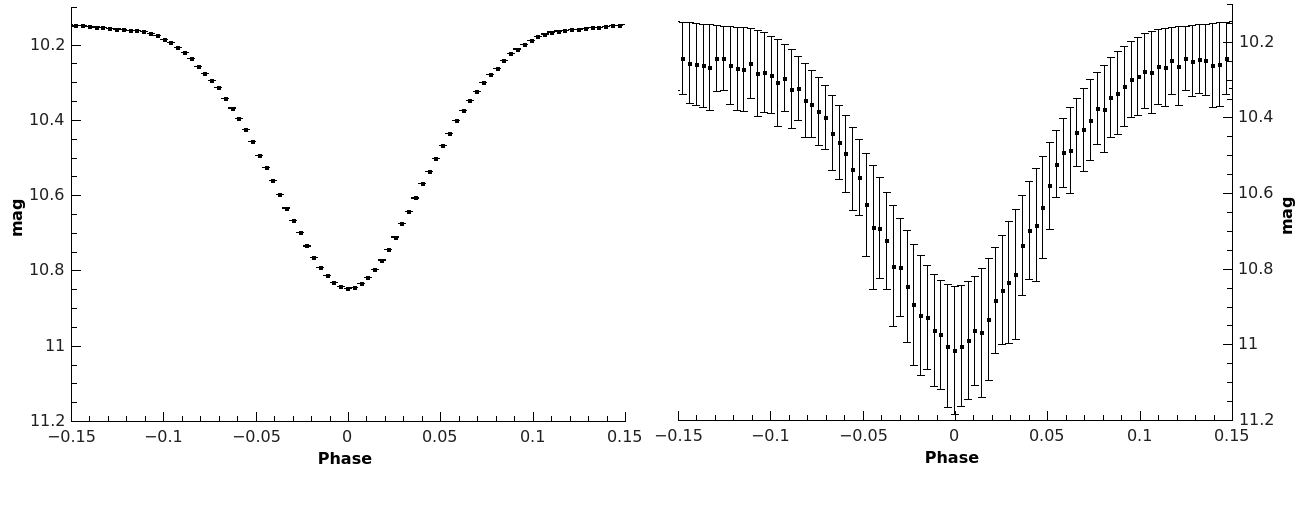
\includegraphics[width=\textwidth]{prec_min//min_err.png}
    \caption{Example of minima with photometry errors 0.0001 mag (left) and 0.1 mag (right)}
    \label{fig:min_err}
\end{figure}

We pick a easiest case -- fitting a classic shape of a minima, and made 1000 simulations of minima determination for both cases. Graphs representing time of minima precision distribution are presented on figure \ref{fig:ph_err_diag}.       

\begin{figure}[!h]
    \centering
    \begin{subfigure}[t]{0.5\textwidth}
        \centering
        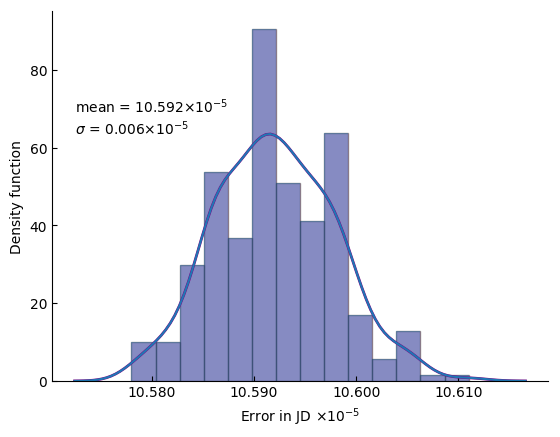
\includegraphics[width=\textwidth]{prec_min//stat_pherr-min.png}
%        \caption{Distribution of errors from LC \\with sampling 20\%}
    \end{subfigure}%
    \begin{subfigure}[t]{0.5\textwidth}
        \centering
        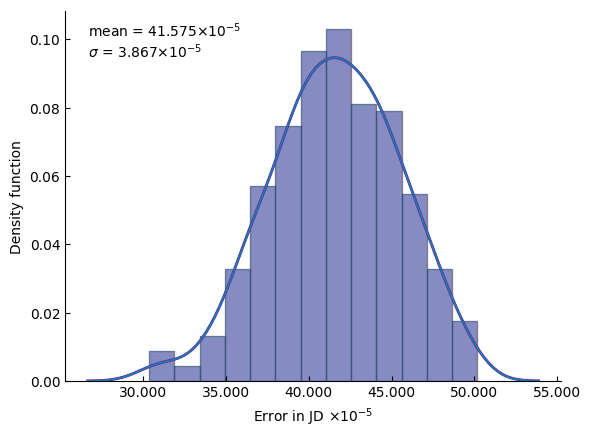
\includegraphics[width=\textwidth]{prec_min//stat_pherr-max.png}
%        \caption{Distribution of errors from LC \\with sampling 80\%}
    \end{subfigure}
    \caption{Distribution of time of minima precision for LC with different photometry accuracy. 0.0001 mag - left, 0.1 mag - right. Blue line is a kernel density estimate.}
\label{fig:ph_err_diag}
\end{figure}
Blue line on figures corresponds to kernel density estimation.
The kernel density estimate (KDE) can be a useful tool for plotting the shape of a distribution. The KDE plots encode the density of observations more clearly then histogram.

As it can be seen from graphs bigger errors (0.1 mag) corresponds to more than two times smaller precision of time of minima determination. Also the standard deviation in case of 0.0001 mag photometry errors is smaller.   

\subsection{Sampling}
According to weather condition, huge errors of photometry, long period of EB system or even some technical issues sampling of data can appear on the light curve.
On next few graphs we will show how sampling affects the precision of minima determination.

As a base we take ideal LC produced by PHOEBE and add the mean photometry error 0.003 mag, which is typical for good weather and telescope with diameter 50 cm with CCD camera. 
We made 1000 simulations of minima determination with random sampling of 20\% of data which is more or less within the bounds of possibility for ground based observations and 1000 simulations of minima determination for 80\% random sampling of data which corresponds to set of bad weather condition or observation of EB system with very long period. 
For example the general look of such LCs are presented on figure \ref{fig:LC_sampl}.

\begin{figure}[!h]
    \centering
    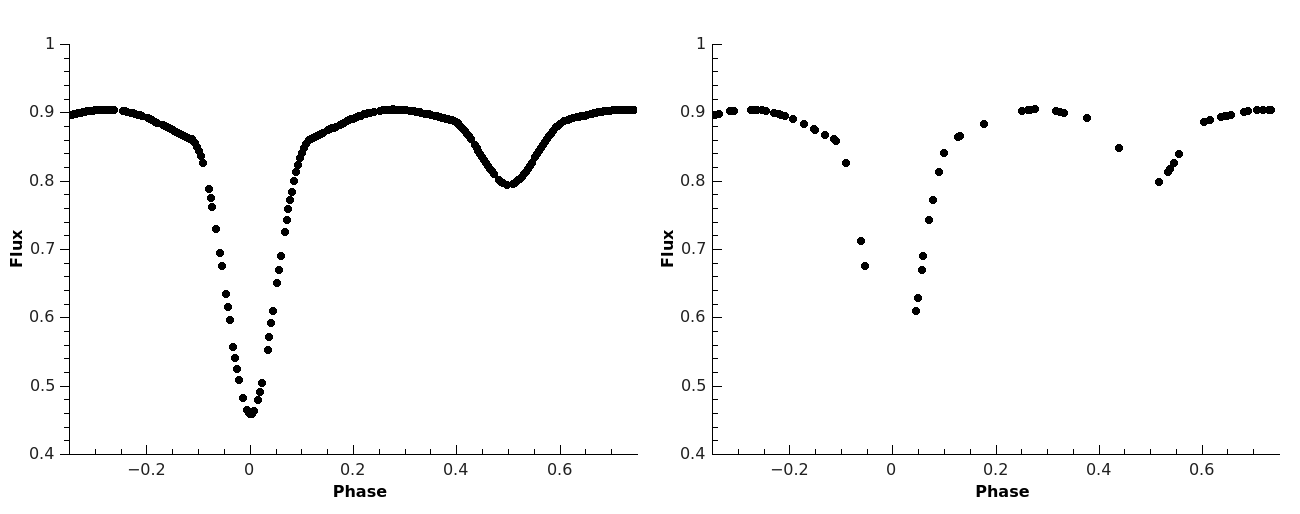
\includegraphics[width=\textwidth]{prec_min//LC_sampl.png}
%    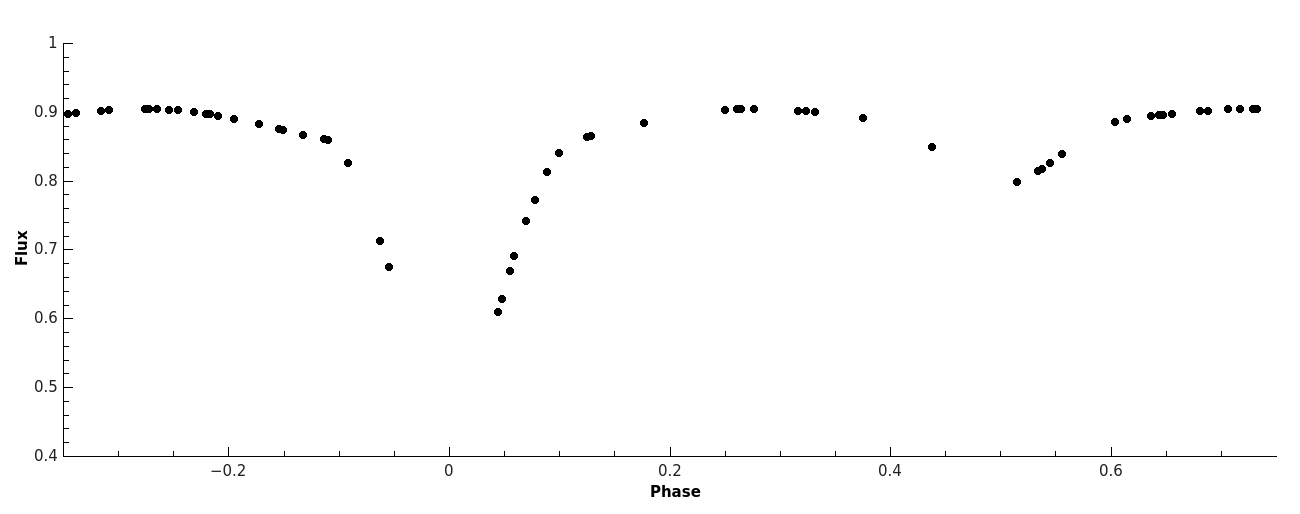
\includegraphics[width=\textwidth]{prec_min//LCs80.png}
    \caption{Example of LC with sampling 20\% (left) and 80\% (right)}
    \label{fig:LC_sampl}
\end{figure}

%\begin{figure}[!h]
%    \centering
%    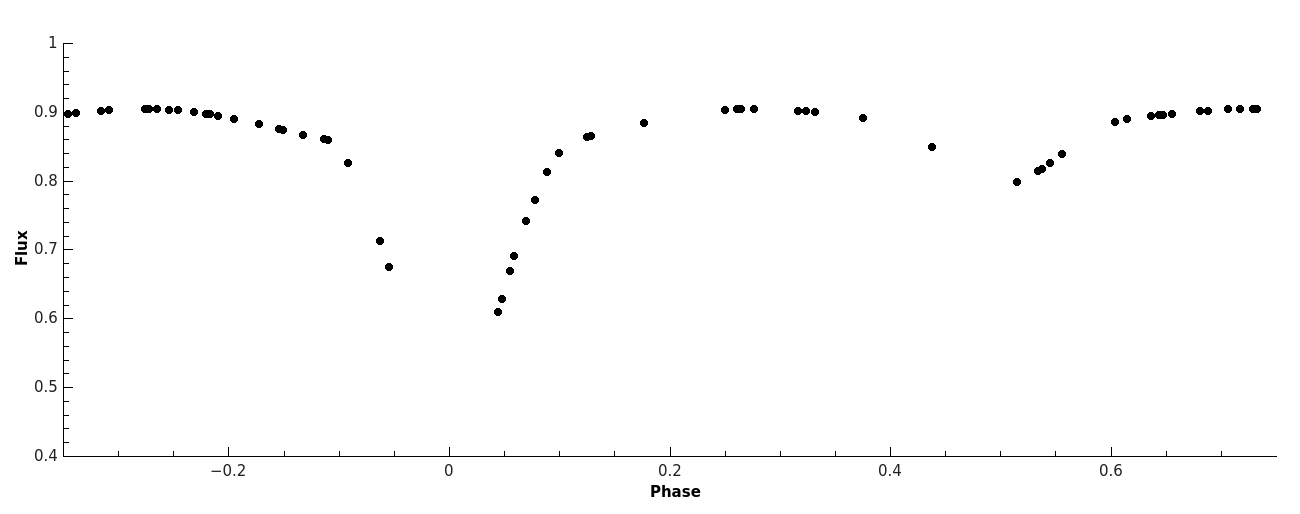
\includegraphics[width=\textwidth]{prec_min//LCs80.png}
%    \caption{LC with sampling 80\%}
%    \label{fig:LC_sampl80}
%\end{figure}

On a figure \ref{fig:sampl_diag} distribution of minima precision is presented for sampling 20\% and 80\%.
Blue line on graph correspond to kernel density estimation.
%The kernel density estimate (KDE) can be a useful tool for plotting the shape of a distribution. The KDE plots encode the density of observations more clearly then histogram.

As it can be expected sampling of data on LC have a great influence on precision of minima determination. 
From Figure \ref{fig:sampl_diag}, we can see that the data with a sampling of 80\% reduces the accuracy of the minimum determination by one order.
%From figure \ref{fig:sampl_diag} we can see that sampling 80\% decrease precision of minima determination in one order.  

\begin{figure}[!h]
    \centering
    \begin{subfigure}[t]{0.5\textwidth}
        \centering
        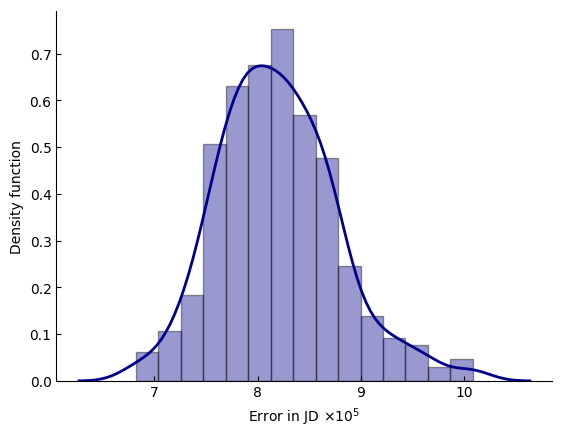
\includegraphics[width=\textwidth]{prec_min//stat-0.2.png}
%        \caption{Distribution of errors from LC \\with sampling 20\%}
    \end{subfigure}%
    \begin{subfigure}[t]{0.5\textwidth}
        \centering
        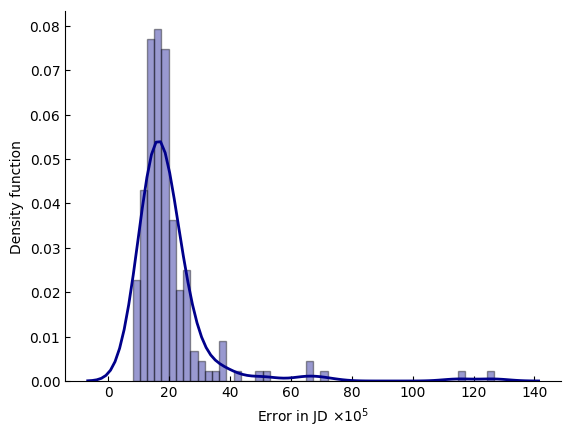
\includegraphics[width=\textwidth]{prec_min//stat-0.8.png}
%        \caption{Distribution of errors from LC \\with sampling 80\%}
    \end{subfigure}
    \caption{Distribution of minima precision from LC with different sampling. 20\% - left, 80\% - right. Blue line is a kernel density estimate.}
\label{fig:sampl_diag}
\end{figure}

%\begin{figure}[!h]
%    \centering
%    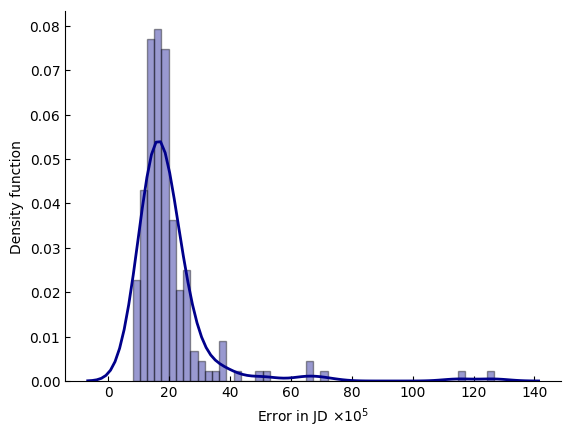
\includegraphics[width=\textwidth]{prec_min//stat-0.8.png}
%    \caption{Distribution of minima precision determinations from LC with sampling 80\%}
%    \label{fig:sampl_diag80}
%\end{figure}
%
%\begin{figure}[!h]
%    \centering
%    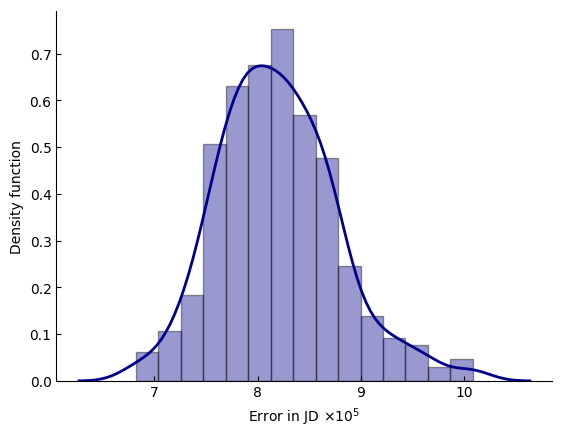
\includegraphics[width=\textwidth]{prec_min//stat-0.2.png}
%    \caption{Distribution of minima precision determinations from LC with sampling 20\%}
%    \label{fig:sampl_diag20}
%\end{figure}

\section{Sampling of data on O-C Diagrams}
5-7 diagrams with different sampling from ideal to few points in different places

\section{Precision of Photometry}
Kepler, Kolonica

\section{Simulations of $3^{rd}$ Body in EB Systems}

In this section, some factors that have an influence on the minima shape, and therefore on O-C diagram too, will be described.  
Such factors are:
\begin{itemize}[noitemsep,nolistsep]
\item EB system visibility from observational point;
\item weather conditions;
\item precision of photometry;
\item presents of spots on EB component, or on both components;
\item pulsation   
\end{itemize}

The O-C diagram of EB system with $3^{rd}$ body would be presented as a ideal conditions case, without any of mentioned above distorting factors, and then compared with conditions close to real one, or under the influence of one of the reviewed factors.

First three factors are not connected with star types, that's why we will consider them separately.
The influence of other factors on O-C diagrams will be considered in the examples of detached and EB contact systems, because of similarity of minima shape in detached, semi-detached and in contact, over-contact EB systems. 

Our simulations are based on a light curves generated by PHOEBE software \citep{Prsa2005} based on well known Wilson \& Devinney code described in work \cite{Wilson1971}. These LC will be extended for needed number of cycles, usually 5 or 10 year. Time shifts in LC caused by presence of $3^{rd}$ body added based on computation made in work \cite{irwin1952, irwin1959}. On the final stage other distortion factors mentioned above are also added to LC.   

\subsection{EB system visibility}

It is good known that periods of star visibility, for some observational point, depend on star declination.
If we proceed from the assumption that observations are collected from one observatory then this feature greatly complicates the task for the observer. In such case there will be only some seasons of observations and gaps in data for a lot of targets. Only near polar regions of sky can be observable throughout the year for middle latitudes observatories.

For example there is two different O-C diagrams presented on Fig. \ref{fig:oc_1}. Left one is for a case when 
target of observation is situated on a equator and right one is for a target near a north pole. Simulations was made for observatory Kolonica AO (Slovakia), duration of observations is 5 years. Parameters of $3^{rd}$ body are presented in second column of table \ref{tab:3rd_body_par}. In a third and fourth columns are orbital parameters obtained by fitting of our O-C diagram with Markov chain Monte Carlo algorithm described in \cite{Gajdos2019}. Same fitting parameters were used for equator and north pole case. We find out that data obtained in the case when the star is situated on the equator are fitted with a worse accuracy and accordingly a star situated near the north pole is fitted better.

\begin{figure}[!h]
    \centering
    \begin{subfigure}[t]{0.5\textwidth}
        \centering
        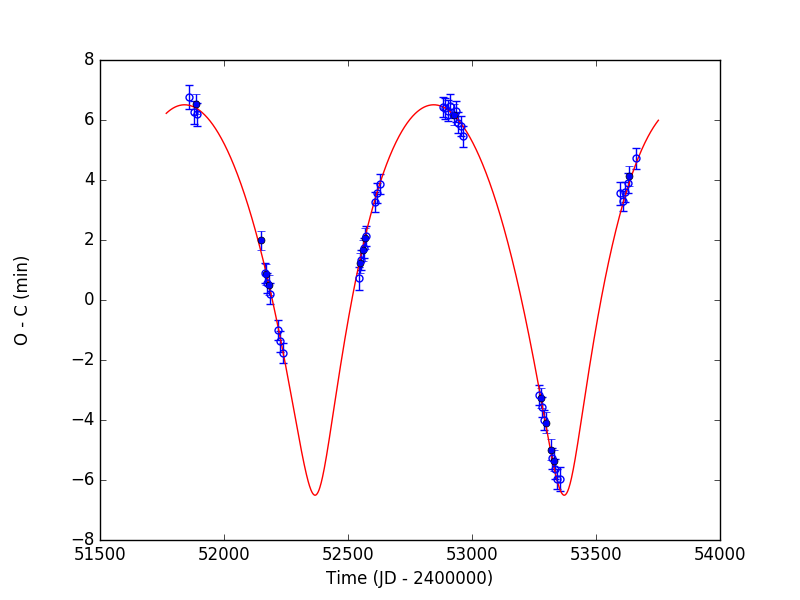
\includegraphics[width=\textwidth]{oc_1_5yrs.png}
        \caption{Star on equator.\\RA = 00:43:45.0838, DEC = +00:00:00}
    \end{subfigure}%
    \begin{subfigure}[t]{0.5\textwidth}
        \centering
        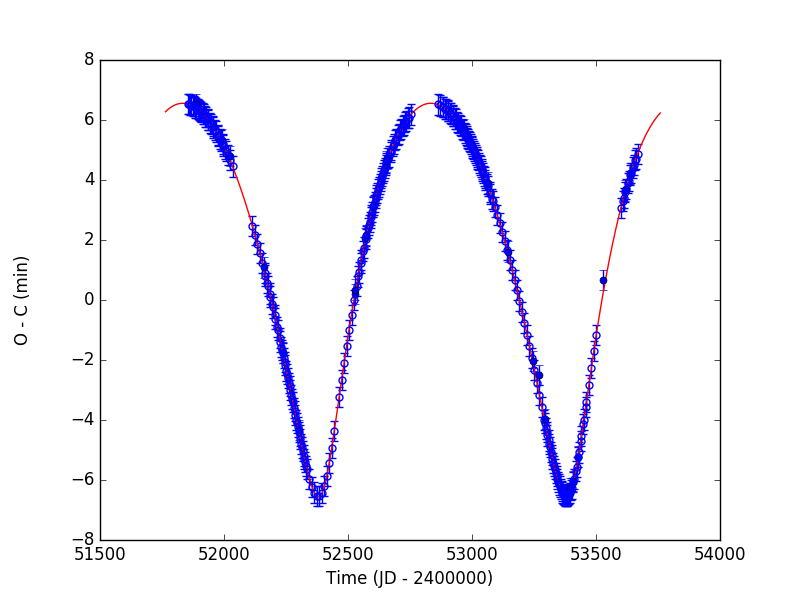
\includegraphics[width=\textwidth]{oc_2_5yrs.png}
        \caption{Star near north pole.\\RA = 00:43:45.0838, DEC = +89:30:00}
    \end{subfigure}
    \caption{O-C diagram for ideal conditions. Red line - fit with MCMC method, correspond to values in table \ref{tab:3rd_body_par}. Filled circles are primary minima, not filled circles - secondary minima. 
    Observatory is Kolonica AO \\(Lat = +48.934917, Lon = 22.2738)}
\label{fig:oc_1}
\end{figure}

\begin{table}[!h]
 \caption{Original parameters of the 3$^{rd}$ body orbit and parameters obtained by fitting $O-C$ diagram simulated in ideal condition on equator and near pole. $P$ -- orbital period of eclipsing pair, $T_0$ -- initial minimum, $P_3$ - orbital period of the 3$^{rd}$ body, $t_{03}$ -- pericenter passage, $a\sin i_3$  -- projected semi-major axis of the orbit, $e_3$ -- eccentricity, $\omega_3$ -- the longitude of the periastron, $f(M_3)$ -- the mass function, $\chi^2$ -- sum of squares of the best fit, $\chi^2/n$ -- reduced sum of squares ($n$ -- number of data points), errors are given in parenthesis.}
 \vspace{-6mm}
 \begin{center}
  \begin{tabular}{lccc}
    \hline
    Solution            & Original                  & Equator               &  near Pole    \\
  \hline\noalign{\smallskip} 
 $P$ [days]             & 1.42834                   & fixed                 & fixed \\ 
 $T_0$ [HJD]            & 2451852.3783              & fixed                 & fixed \\
   \hline\noalign{\smallskip} 
 $P_3$ [days]           &   1000                    & 997(3)                & 999.90(92)\\
 $t_{03}$ [HJD]         & 2451400                   & 2451407(9)            & 2451400(1)    \\
$a\sin i_3$ [AU]        &  0.797                    & 0.807(15)             & 0.8001(35)\\
 $e_3$                  &  0.54                     & 0.55(1)               & 0.5449(45)\\
$\omega_3$ [\degree]    &   288                     & 289(3)                & 288.16(76)\\
\hline\noalign{\smallskip}
$f(M_3)$  [M$_\odot$]   &  --                       & 0.070(4)              & 0.06835(91)\\
\hline\noalign{\smallskip}
$\chi^2$                &  --                       & 8.34                  & 8.323\\
$\chi^2/n$              &  --                       & 0.19                  & 0.026\\
\hline\noalign{\smallskip}
\end{tabular}
\end{center}
\label{tab:3rd_body_par}
\vspace{-6mm}
\end{table}

\subsection{Weather and Photometry Precision}
If we will take into account other factors, like weather and precision of photometry, we will probably get less fit accuracy. 
On the Fig.\ref{fig:oc_weather} (a, b) are presented O-C diagrams with same EB system as in previous case but now we take into account only 45\% of good weather, and photometry precision 0.0001. Such weather condition are rather good for our latitudes, photometry precision 0.0001 can be achieved on 400-600 mm telescopes with modern CCD cameras. Obtained parameters of $3^{rd}$ body orbit are presented in table \ref{tab:3rd_body_w}.

As we can se in table \ref{tab:3rd_body_w}, for a case when star is on equator difference with ideal condition is not so big on $\chi^2/n$ but accuracy of individual parameters is worse. It is because there is not much data point at all for this case.
On the other hand situation for a case when star is near the pole, in comparison with ideal conditions, is getting much worse. 

If we do a simulation of O-C diagrams with more appropriate for our latitudes 30 \% probability of clear sky, values are getting worse. This results are presented on Fig. \ref{fig:oc_weather} (c,d) and in table \ref{tab:3rd_body_w}.

In real life for research of some EB system light curves from many different observatories are used. If this observatories are situated on different latitudes then we will not have such big gaps in our data as can be seen for a case of star on equator. The more observatories contribute to research the less important is influence of weather conditions and object location.
% Weather and photom precision-----------------------------------------
\begin{figure}[!h]
    \centering
    \begin{subfigure}[t]{0.5\textwidth}
        \centering
        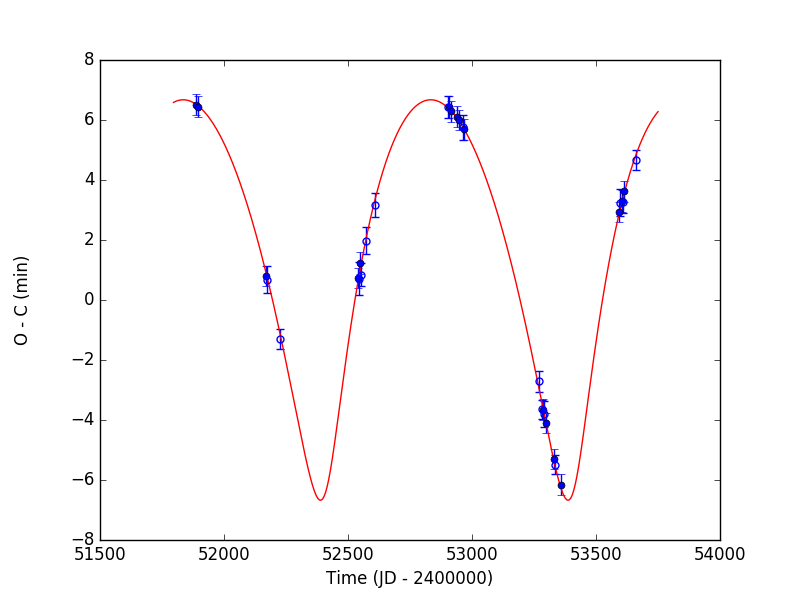
\includegraphics[width=\textwidth]{oc_w.png}
        \caption{Star on equator. 45\% of clear nights.\\RA = 00:43:45.0838, DEC = +00:00:00}
    \end{subfigure}%
    \begin{subfigure}[t]{0.5\textwidth}
        \centering
        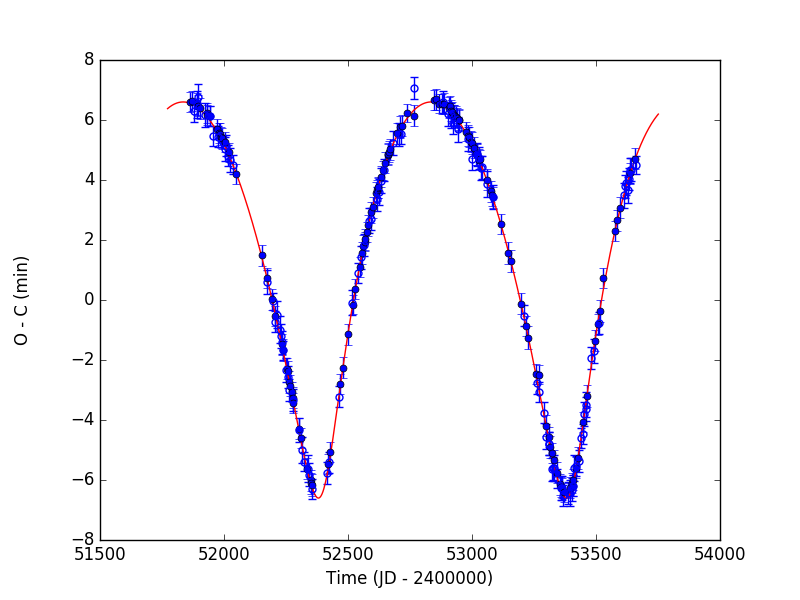
\includegraphics[width=\textwidth]{oc_eq_w2.png}
        \caption{Star near north pole. 45\% of clear nights\\RA = 00:43:45.0838, DEC = +89:30:00}
    \end{subfigure}
    
    \begin{subfigure}[t]{0.5\textwidth}
        \centering
        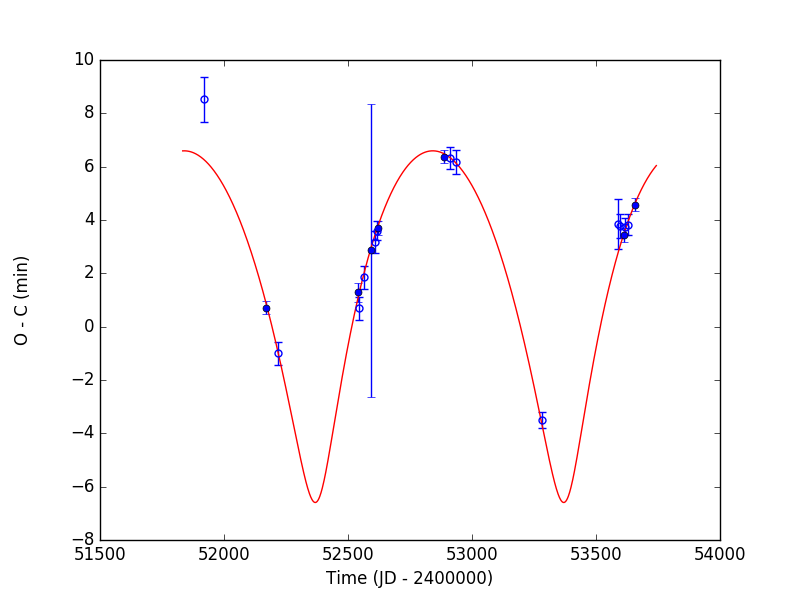
\includegraphics[width=\textwidth]{oc_w30_e.png}
        \caption{Star on equator. 30\% of clear nights\\RA = 00:43:45.0838, DEC = +00:00:00}
    \end{subfigure}%
    \begin{subfigure}[t]{0.5\textwidth}
        \centering
        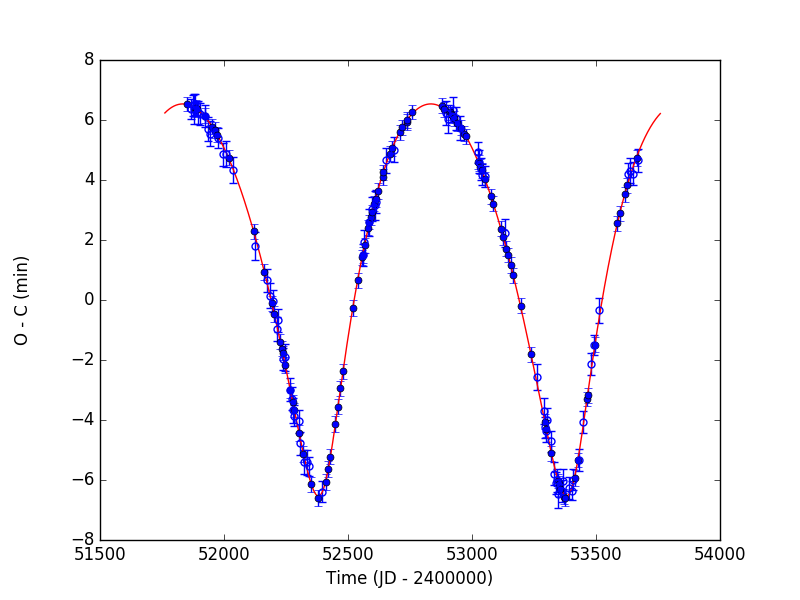
\includegraphics[width=\textwidth]{oc_w30_p.png}
        \caption{Star near north pole. 30\% of clear nights\\RA = 00:43:45.0838, DEC = +89:30:00}
    \end{subfigure}
    \caption{O-C diagram for 45\% (a,b) and 30\% (c,d) of good weather and photometry accuracy 0.0001.
    Red line - fit with MCMC method, correspond to values in table \ref{tab:3rd_body_w}. Filled circles are primary minima, not filled circles - secondary minima. Observatory is Kolonica AO \\(Lat = +48.934917, Lon = 22.2738)}
\label{fig:oc_weather}
\end{figure}


\begin{table}[!h]
 \caption{Original parameters of the 3$^{rd}$ body orbit and parameters obtained by fitting $O-C$ diagram simulated with influence of weather (45\% and 30\% of clear nights) and photometry precision 0.0001. For description of parameters see Table \ref{tab:3rd_body_par}}
 \vspace{-6mm}
 \begin{center}
  \begin{tabular}{lccccc}
    \hline
    Solution            & Original                  & Equator 45 \%         &  Pole 45\%          & Equator 30\%  &  Pole 30\%        \\
  \hline\noalign{\smallskip}                                                                                                                 
 $P$ [days]             & 1.42834                   & fixed                 & fixed               & fixed        & fixed             \\ 
 $T_0$ [HJD]            & 2451852.3783              & fixed                 & fixed               & fixed        & fixed             \\
   \hline\noalign{\smallskip}                                                                                                         
 $P_3$ [days]           &   1000                    & 998(4)                & 1000(1)             & 1002(5)      & 999(1)            \\
 $t_{03}$ [HJD]         & 2451400                   & 2451413(11)           & 2451398(3)          & 2451376(16)  & 2451399(3)       \\
$a\sin i_3$ [AU]        &  0.797                    & 0.819(22)             & 0.805(4)            & 0.797(22)    & 0.801(5)          \\
 $e_3$                  &  0.54                     & 0.553(14)             & 0.5588(57)          & 0.569(23)    & 0.558(6)        \\
$\omega_3$ [\degree]    &   288                     & 291(5)                & 287.6(9)            & 280(5)       & 289(1)          \\
\hline\noalign{\smallskip}                                                                                                                   
$f(M_3)$  [M$_\odot$]   &  --                       & 0.074(6)              & 0.069(1)            & 0.067(6)     & 0.069(1)          \\
\hline\noalign{\smallskip}                                                                                                               
$\chi^2$                &  --                       & 4.82                  & 36.46               & 15.00        & 31.29              \\
$\chi^2/n$              &  --                       & 0.18                  & 0.16                & 1.00         & 0.18              \\
\hline\noalign{\smallskip}

\end{tabular}
\end{center}
\label{tab:3rd_body_w}
\vspace{-6mm}
\end{table}

\subsection{Spots in EB Systems}
In previous subsections, we were dealing with terrestrial factors that cause inaccuracy in O-C diagrams. 
Now we will try to simulate O-C diagrams in ideal terrestrial conditions but under the influence of other non-terrestrial factors like starspots.

As we know the formation of starspots depends on the age of a host star, that's why we should separate our simulation on detached and contact EB systems. 
But before we start to simulate we need to know some general spot parameters for this EB systems. Its a radius of star spot, its temperature, and life cycle. Do the spot disappear after some short time or can be present on a host star for a relatively long time like 5-10 years? The spots migrate or not?  

In work \cite{Kalimeris2002} authors have
shown that intensity variations resulting from star-spots (not taking into account Wilson depressions) can introduce disturbances of
up to $\sim 0.01$~day in the O-C residuals of contact binaries. Given the
rapid evolutionary time-scales of spots (of the order of days) seen in
recent Doppler images of the contact binary AE Phe \citep{Barnes2004} 
this may lead to explaining some of the observed jitter in the
O-C curves of these objects. But in work \cite{Watson2004}, the effects of a
Wilson depression seem to result in a scatter of only a few seconds
in the O-C residuals, it seems unlikely that the Wilson depression
will be a significant source of jitter for contact binaries.
Such changes resulting from star-spots
would be distinguishable from other mechanisms that cause period
changes and it should still be possible to determine the orbital period accurately  \citep{Watson2004}.

Several studies have indicated that spot on close binaries can have angular diameters from $10\degree$ to $40\degree$ which means that they
will cover from 5 to 25\% of the whole photosphere of the active components (e.g. \cite{Hall1990, Guinan1993}).
In most cases, active component can have one or two giant spots. It is also argued that such spots can remain on a surface from a few years to even ten years \citep{Kalimeris2002}. 

For a estimation of maximum effect caused by the star spot, it is assumed that in our simulations spots are located on equator of each component.
According to \cite{Kalimeris2002} spots with angular diameter less then $10\degree$ cause negligible shifts of the light minimum of the primary eclipse. Therefore we will not consider with spots smaller then $10\degree$ (see fig. \ref{fig:spot_diam}).

Furthermore, the spots on secondary component always remain visible during the primary eclipse,
while the spots on primary do not. As a result, the spots on primary cause a
significantly greater photometric perturbation to the light curve than the spots on secondary component.

\citeauthor{Kalimeris2002} also showed that unlike real orbital period changes, non-migrating star spots cannot
cause permanent slopes in the O-C diagrams. 
But the O-C differences caused by long-lived migrating spots can be expected to be periodic.

\begin{figure}[!h]
\vspace{0cm}
\centerline{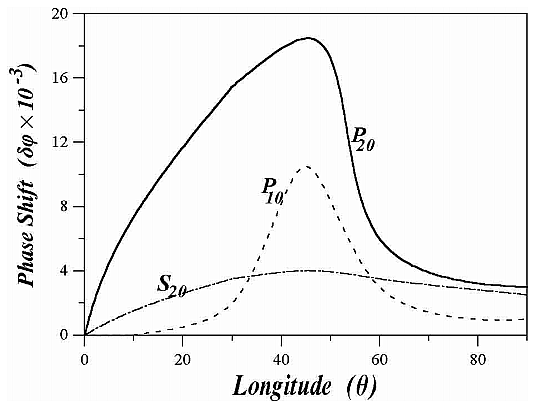
\includegraphics[width=0.60\textwidth]{spot_diam_2.png}}
\caption{Phase shift $\delta\varphi(\theta)$ of the primary eclipse of a contact
binary similar to AB And. Curves labelled by "P" correspond
to a spot on the primary, while "S" refers to a spot on the
secondary component. \citep{Kalimeris2002}.}
\label{fig:spot_diam}
\end{figure}   
 

\subsubsection{Detached EB Systems}
% Pro single stars
%Younger stars rotate faster than older stars and
%have higher activity levels and greater spot coverage (????). As a result, there is an overall trend of the
%degree of photometric variability with age. % \cite article "The Ages of Stars".

Tidal interactions force most of these stars to rotate synchronously with their orbital motions.
The rapid rotation combined with deep convection envelopes produces a variety of magnetic activity phenomena including starspots in these stars.

Brightness variations due to starspots can be observed in detached EB only during primary total eclipses when the luminous hot components are hidden. Therefore, because of synchronized rotation, only one hemisphere of the cool stars can be observed and the photometric data collected are less detailed than for other spotted binaries \citep{Berdyugina2005}.
 
For detached eclipsing binary systems spots with radius from 5\degree~to~25\degree are usually typical, we can find such systems in many publications like e.g. \cite{Liakos2011} or in publications about spots in RSCVn binaries systems (e.g. \cite{Roettenbacher2011, Kovari2012, Kozhevnikova2015}). Objects with spots migrations are very rarely observed, so we will not consider such a case.
Model of detached EB system is presented on figure \ref{fig:eb_det_model}, the main parameters of this system are listed in the table \ref{tab:detached_params}.

As we mentioned above, spots with a radius less then 10\degree~ do not have a big influence on O-C diagram. So, we will consider how starspot located on stars equator (colat=90\degree, lon=0\degree) with radius $r_{spot}=15\degree$ and $r_{spot}=25\degree$~ affect the O-C diagram. 
There is also a difference in a hot and cold spot. The hot spot will have $T_{spot}=1.2$, where $T_{spot}$ is the ratio between the temperature of the spot and the local temperature of the underlying photosphere, the cold spot will be defined as $T_{spot}=0.8$. On figure \ref{fig:detached_spots} we can see how hot and cold spots affect the shape of the minima. Mainly primary minima are changing their shape under the influence of spots.

\begin{figure}[!h]
\vspace{0cm}
\centerline{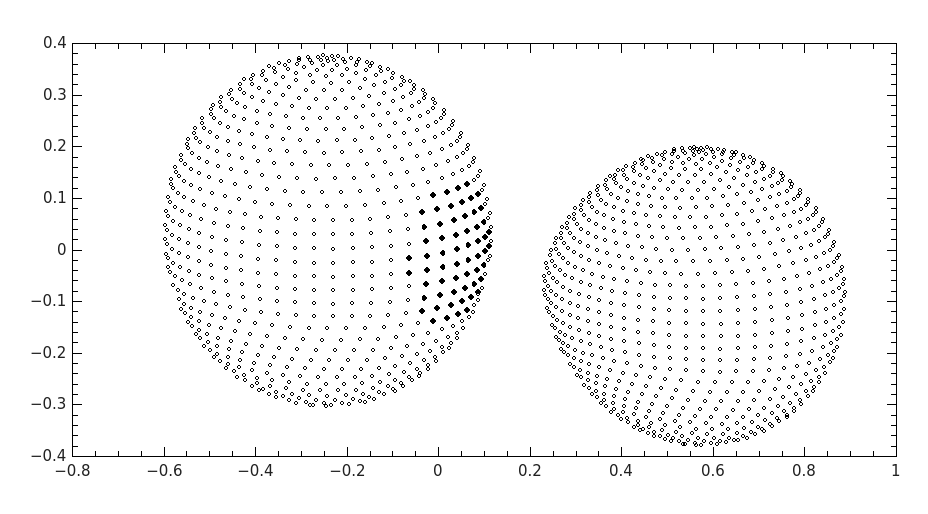
\includegraphics[width=0.80\textwidth]{detached_pspot_08-25_view.png}}
\caption{Model of detached EB system with spot (colat=90\degree, colon=0\degree) in plane of sky view at phase 0.15.}
\label{fig:eb_det_model}
\end{figure}

\begin{table}[!h]
 \caption{Basic parameters of detached binary system presented on figure~ \ref{fig:eb_det_model}. HJD0 is a origin of the
 ephemeris; P - orbital period of EB system; SMA - semi-major axis; RM - mass ratio; VGA - centre of mass velocity, \\INCL - inclination}
 \begin{center}
 \vspace{-6mm}
  \begin{tabular}{c|c}
    \hline 
HJD0(day) & 2451852.3783\\
P(day)    & 1.42834\\
\hline
SMA ($R_\odot$) &  1.000\\
RM              &  0.432\\
VGA (km/s)      &  0\\
INCL (\degree)  & 77.690\\
\hline
\end{tabular}
\end{center}
\label{tab:detached_params}
\vspace{-6mm}
\end{table}

\begin{figure}[!h]
    \centering
    \begin{subfigure}[t]{0.5\textwidth}
        \centering
        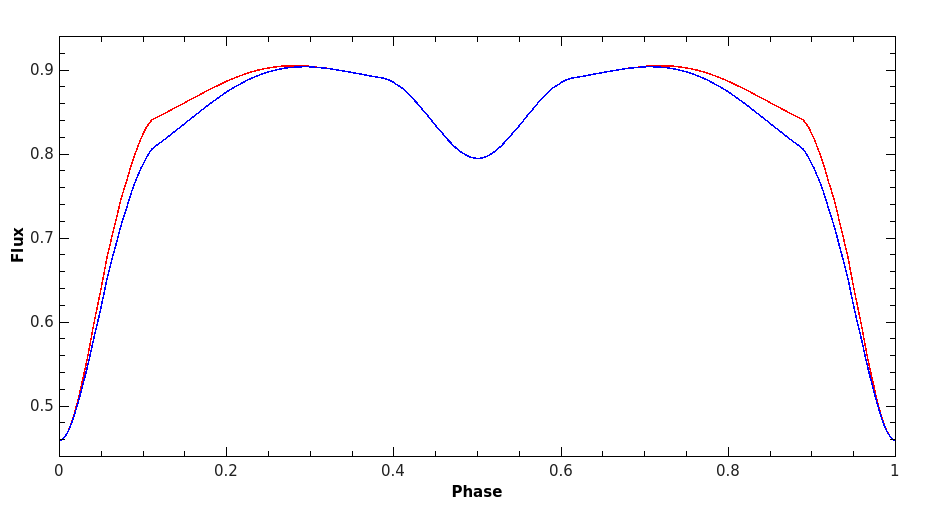
\includegraphics[width=\textwidth]{detached_pspot_08.png}
        \caption{Spot with $T_{spot}=0.8$}
    \end{subfigure}%
    \begin{subfigure}[t]{0.5\textwidth}
        \centering
        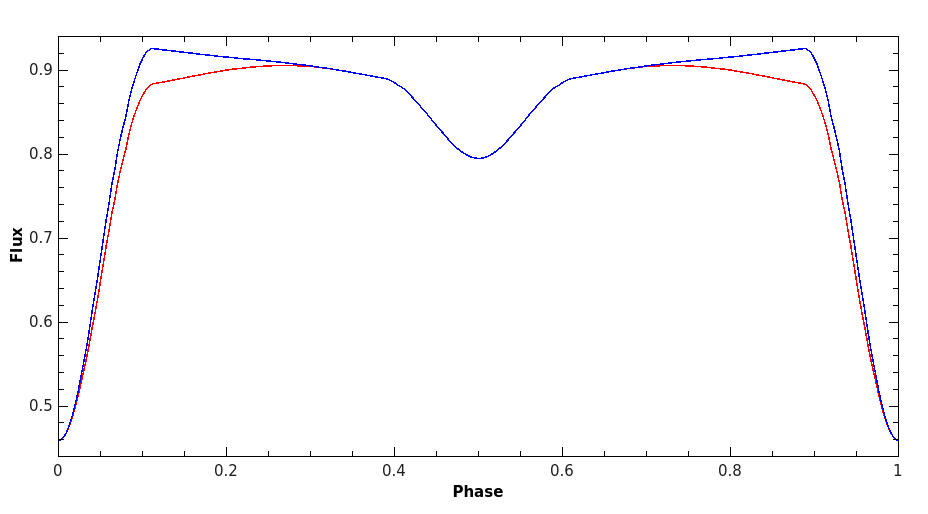
\includegraphics[width=\textwidth]{detached_pspot_12.png}
        \caption{Spot with $T_{spot}=1.2$}
    \end{subfigure}
    \caption{Spot on primary component with different temperature and radius. 
    Blue line - spot radius 25\degree, red line - spot radius 15\degree}
\label{fig:detached_spots}
\end{figure}

The final O-C diagrams for all four cases are presented in figure \ref{fig:oc_detached_spot}. Looking only on O-C diagram we can't clearly see the difference. Only when we fit these O-C diagrams by MCMC method results are getting clearer. 
Final solutions of fitting are presented in table \ref{tab:3rd_body_detached_spot}. Analysing $\chi^2$ value of 4 cases we can state that 
case of spot with parameters $T_{spot}=1.2$ and $r_{spot}=25\degree$ is fitted the best. The precision of fit depends on the accuracy of minima determination that can vary depending on the method we used. In case of a spot with parameters $T_{spot}=1.2$ and $r_{spot}=25\degree$ precision of minima determination was almost the same for primary and secondary minima. 

%are almost the same, except case of spot with $T_{spot}=1.2$ and $r_{spot}=25\degree$, in this case $\chi^2$ is the best. 
%But if we take into account Bayesian information criterion (BIC) and Akaike information criterion (AIC), where bigger value corresponds to better fit, the situation changes to the opposite. 
%Best fit is case with small cold spot, and worst fit is case with hot and big spot.\\
%(RECALCULATE!!!!!) 

\begin{figure}[!h]
    \centering
    \begin{subfigure}[t]{0.5\textwidth}
        \centering
        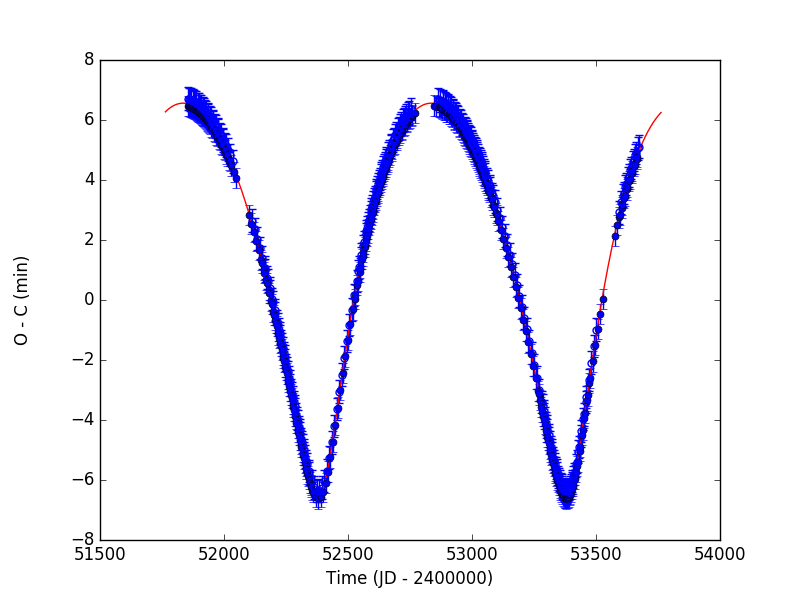
\includegraphics[width=\textwidth]{oc_detached_pspot_R15_T12.png}
        \caption{O-C diagram with $r_{spot}=15, T_{spot}=1.2$}
    \end{subfigure}%
    \begin{subfigure}[t]{0.5\textwidth}
        \centering
        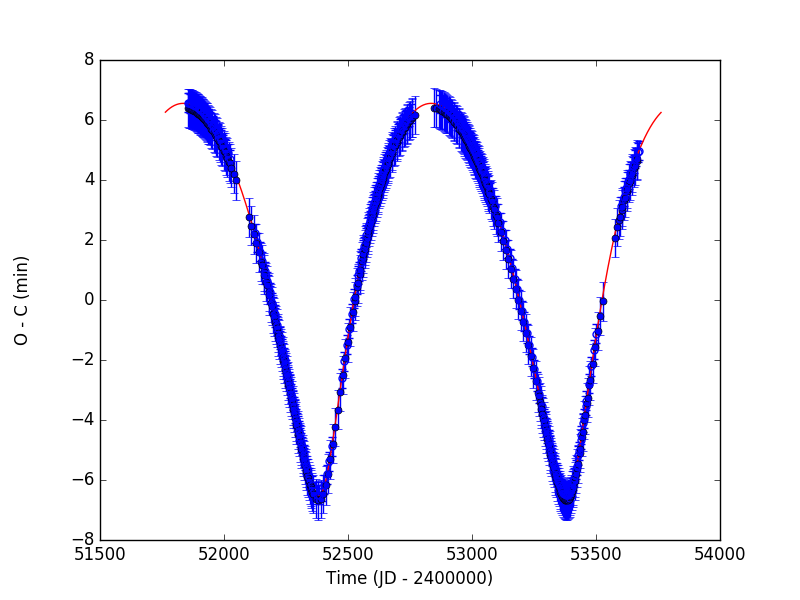
\includegraphics[width=\textwidth]{oc_detached_pspot_R25_T12.png}
        \caption{O-C diagram with $r_{spot}=25, T_{spot}=1.2$}
    \end{subfigure}
    
    \begin{subfigure}[t]{0.5\textwidth}
        \centering
        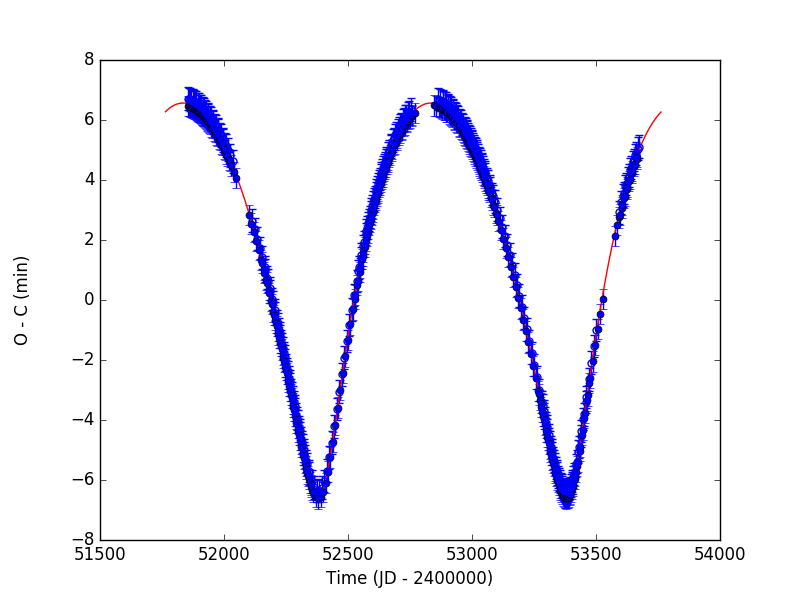
\includegraphics[width=\textwidth]{oc_detached_pspot_R15_T08.png}
        \caption{O-C diagram with $r_{spot}=15, T_{spot}=0.8$}
    \end{subfigure}%
    \begin{subfigure}[t]{0.5\textwidth}
        \centering
        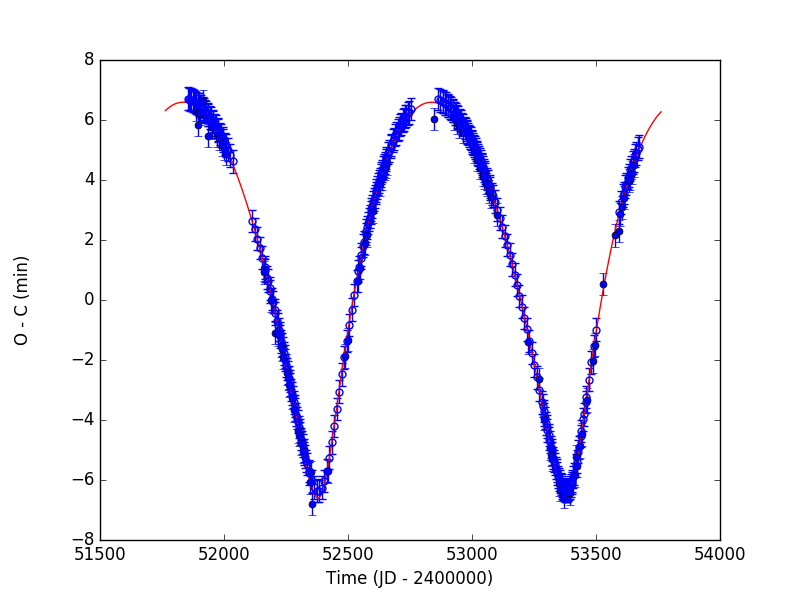
\includegraphics[width=\textwidth]{oc_detached_pspot_R25_T08.png}
        \caption{O-C diagram with $r_{spot}=25, T_{spot}=0.8$}
    \end{subfigure}
    \caption{O-C diagram for EB system with different $r_{spot}$ and $T_{spot}$\\
    Red line - fit with MCMC method, correspond to values in table \ref{tab:3rd_body_detached_spot}. 
    Filled circles are primary minima, not filled circles - secondary minima.}
\label{fig:oc_detached_spot}
\end{figure}


\begin{table}[!h]
 \caption{Orbital parameters of $3^{rd}$ body for detached EB system with different spot parameters $r_{spot}$ and $T_{spot}$. 
 For description of parameters see Table~\ref{tab:3rd_body_par}}
  \vspace{-6mm}
 \begin{center}
  \begin{tabular}{lccccc}
    \hline
    Solution            & Original       & $r_{spot}$=25\degree&$r_{spot}$=25\degree  &$r_{spot}$=15\degree &$r_{spot}$=15\degree \\
                        &                &    $T_{spot}$=1.2    &  $T_{spot}$=0.8 &  $T_{spot}$=1.2  &  $T_{spot}$=0.8 \\
  \hline\noalign{\smallskip}                                                                                                                 
 $P$ [days]             & 1.42834        &           fixed     & fixed       & fixed        & fixed       \\ 
 $T_0$ [HJD]            & 2451852.3783   &           fixed     & fixed       & fixed        & fixed       \\
   \hline\noalign{\smallskip} 
% $P_3$ [days]           &   1000         &          999.9(9)   & 1001(1)     &   1000.7(9)  &  999.8(7)   \\       
% $t_{03}$ [HJD]         & 2451400        &          2451400(2) & 2451394(2)  &   2451397(2) &  2451400(1) \\
%$a\sin i_3$ [AU]        &  0.797         &          0.799(3)   & 0.803(3)    &   0.799(3)   &  0.801(2)   \\     
% $e_3$                  &  0.54          &          0.541(4)   & 0.566(5)    &   0.548(3)   &  0.547(3)   \\            
%$\omega_3$ [\degree]    &   288          &          287.8(7)   & 286.6(8)    &   287.4(8)   &  288.0(5)   \\     
%\hline\noalign{\smallskip}                                                                                                 
%$f(M_3)$  [M$_\odot$]   &  --            &          0.0681(8)  & 0.0689(9)   &   0.0681(7)   &  0.0686(7)  \\       
%\hline\noalign{\smallskip}                                                                                             
%$\chi^2$                &  --            &          21.714     & 54.867      &  74.652      &  74.168     \\        
%$\chi^2/n$              &  --            &           0.0347    & 0.1432      &   0.1161     &   0.1153    \\ 
                                                                                                        
 $P_3$ [days]           &   1000         &          1000(1)    & 1000.0(7)   &   1000(1)    &  1000.8(9)   \\       
 $t_{03}$ [HJD]         & 2451400        &          2451397(3) & 2451397(1)  &   2451396(2) &  2451396(2) \\
$a\sin i_3$ [AU]        &  0.797         &          0.801(2)   & 0.803(3)    &   0.806(4)   &  0.802(3)   \\     
 $e_3$                  &  0.54          &          0.552(3)   & 0.559(4)    &   0.572(5)   &  0.563(3)   \\            
$\omega_3$ [\degree]    &   288          &          287.2(8)   & 287.1(6)    &   286.9(8)   &  286.9(7)   \\     
\hline\noalign{\smallskip}                                                                                                 
$f(M_3)$  [M$_\odot$]   &  --            &          0.0685(7)  & 0.0690(7)   &   0.0697(10) &  0.0691(7)  \\       
\hline\noalign{\smallskip}                                                                                             
$\chi^2$                &  --            &          7.326      & 35.990      &  30.227      &  39.209     \\        
$\chi^2/n$              &  --            &           0.0127    & 0.0654      &   0.0767     &   0.0993    \\       
% AIC                    &  --            &          31.714     & 64.867      &  84.652      &  84.168     \\
% BIC                    &  --            &          53.942     & 84.672      & 107.022      & 106.538     \\
\hline\noalign{\smallskip}  

\end{tabular}
\end{center}
\label{tab:3rd_body_detached_spot}
\vspace{-6mm}
\end{table}

It was mentioned above that spot on secondary component do not have a big influence on minima shape, so we will not consider here this option.

As a conclusion we can say that detached EB systems with spot are not sophisticated objects for $3^{rd}$ body detection. In case of bigger then 25\degree ~spots on the surface it is advisable to cut off from the top the height of primary (or secondary) minima to get better fit and to determine the time of minima more precisely.
 
\subsubsection{Contact EB Systems}
Contact binary stars occur relatively often among binaries (95\% of eclipsing binary
variables in the solar neighbourhood) \cite{Rucinski98}. 
A contact binary system consists of two dwarf stars, most often from the F, G, and K
spectral classes, that are surrounded by a common convective envelope. 
The orbital period distribution peaks in the 8 to 12 hour range. Most systems, though not all,
have orbital periods between 0.2 and 1.0 days \citep{Maceroni96, Paczynski2006}. 
While the masses of the two component stars of a contact binary
are typically unequal, the two stars usually have approximately equal surface temperatures due to the effects of
mass and energy transfer between the components via a common convective envelope \citep{Lucy68}. 
Eclipsing contact binaries are often referred to as W UMa systems in honor of the prototype \citep{Tran2013}.

The components of such a contact binary rotate very rapidly in spite of their old ages
($v~sin~i \sim 100 - 200~ km~s^{-1}$ ) as a result of spin-orbit synchronisation due to strong tidal interactions between the stars \citep{Berdyugina2005}. 

%Observations reveal that there are two subclasses of W UMa stars: A-type and W-type systems.
%The former have longer periods, are hotter, have larger total mass, and a smaller mass-ratio and
%are in better contact.
Many contact binaries show signs of stellar activity, presumably because the component stars are rapid
rotators with deep convective zones. 
A study of the contact binaries with Doppler imaging
technique reveals that both components can be covered by cool starspots, with
a tendency for the primary to be more active than the secondary \citep{Maceroni94, Hendry2000, Barnes2004}.

This makes contact binaries excellent laboratories in
which to investigate the temporal variations and evolution of stellar spots, in part because the timescales of
the variations are shorter than in other types of binary and single stars. 
However, the shortest among these timescales can be problematic to study using groundbased observatories because they are comparable to the
length of an Earth night.

\begin{figure}[!h]
\vspace{0cm}
\centerline{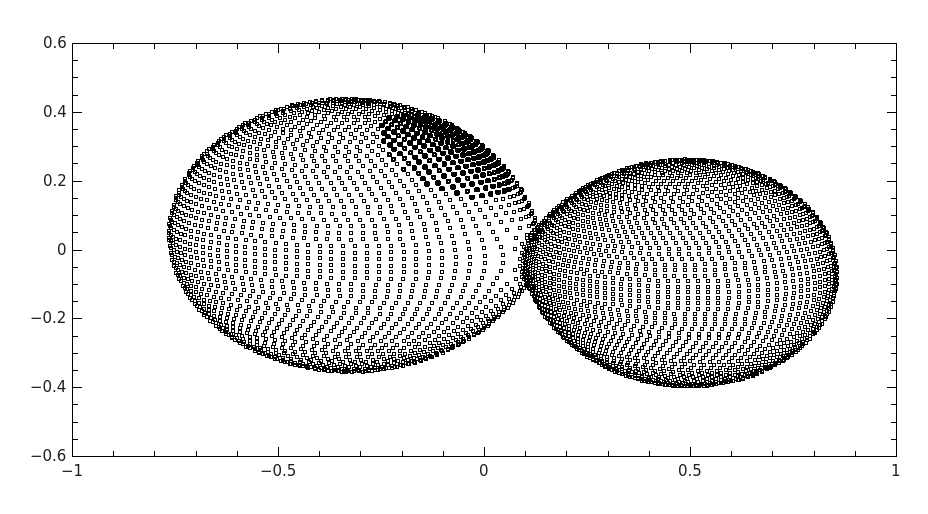
\includegraphics[width=0.8\textwidth]{Overcontact_mesh.png}}
\caption{Model of contact EB system with spot (colat=45\degree, colon=0\degree) in plane of sky view at phase 0.15.}
\label{fig:eb_overcont_model}
\end{figure}


\begin{table}[!h]
 \caption{Baisic parameters of contact binary system presented on figure~ \ref{fig:eb_overcont_model}. HJD0 is a origin of the
 ephemeris; P - orbital period of EB system; SMA - semi-major axis; RM - mass ratio; VGA - centre of mass velocity, \\INCL - inclination}
 \begin{center}
 \vspace{-6mm}
  \begin{tabular}{c|c}
    \hline 
HJD0(day) & 2451852.3783\\
P(day)    & 1.42834\\
\hline
SMA ($R_\odot$) &  1.76\\
RM              &  0.67\\
VGA (km/s)      &  4.70\\
INCL (\degree)  & 79.50\\
\hline
\end{tabular}
\end{center}
\label{tab:overcontact_params}
\vspace{-6mm}
\end{table}

\cite{Kalimeris2002} noted that the migration of
starspots on the surface(s) of the constituent stars in
short-period binaries, especially contact binaries, could
affect measurements of eclipse times and thereby mimic
changes in the orbital period \citep{Tran2013}. 
%\cite{Kalimeris2002} also
%showed that the perturbations to the O-C diagrams would generally have amplitudes smaller than $\sim 0.01$ days, and could appear to
%be quasiperiodic on timescales of a few hundred days or so if the spot migration is related to differential rotation
%of the host star \citep{Tran2013}.

Model of contact EB system with spot is presented on figure \ref{fig:eb_overcont_model}, orbital parameters can be found in table \ref{tab:overcontact_params}. 

\begin{figure}[!h]
    \centering
    \begin{subfigure}[t]{0.5\textwidth}
        \centering
        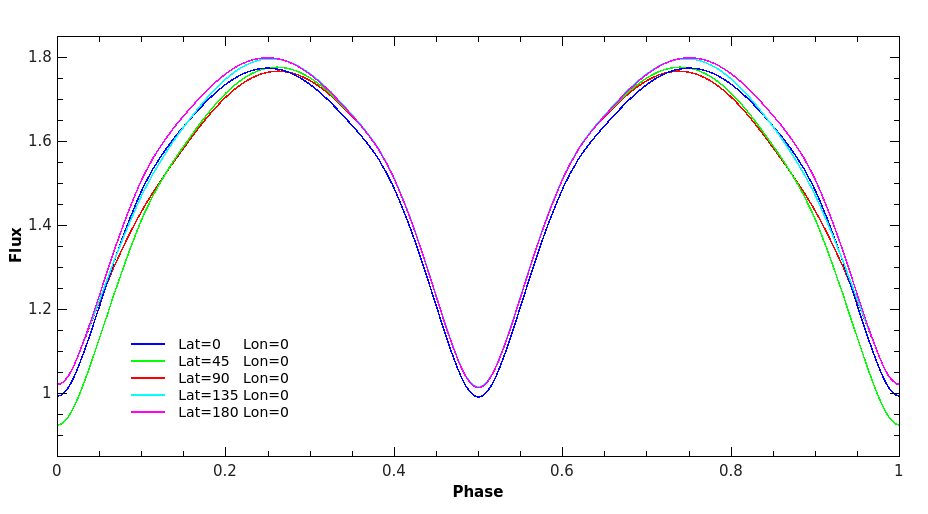
\includegraphics[width=\textwidth]{Overc_spot_pos_lat.png}
        \caption{LC with spot on different colatitude and \\longitude = 0\degree}
    \end{subfigure}%
    \begin{subfigure}[t]{0.5\textwidth}
        \centering
        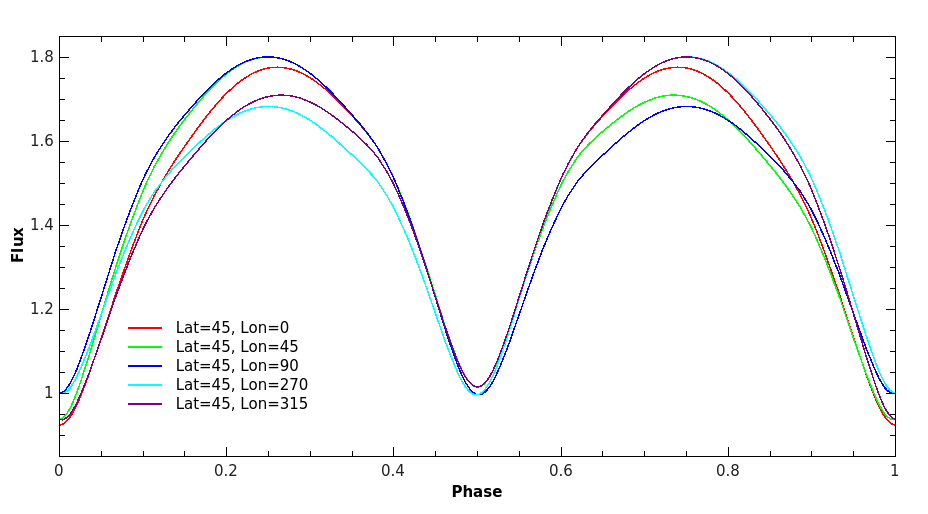
\includegraphics[width=\textwidth]{Overc_spot_pos_lon.png}
        \caption{LC with spot on different longitude and \\colatitude = 45\degree}
    \end{subfigure}
    \caption{LC of contact binary system with "cold" spot ($T_{spot}=0.8~T_{surf}$) on primary component at different positions}
\label{fig:overcontact_spot_pos}
\end{figure}

Light curve from such EB system will be subjected to changes depending on the position of the spot, such changes are partially presented on figure \ref{fig:overcontact_spot_pos}, \ref{fig:overcontact_spotT12_pos}. Analyzing these data we can conclude that the most noticeable changes in LC are caused by changes of position in longitude of a starspot on the primary component of contact binary EB system.
If we change spot position only in colatitude and leave longitude equal to 0\degree, we will observe only variation of primary minima shape and depth. On the other hand if we make colatitude constant (colatitude = 45\degree~ on figures \ref{fig:overcontact_spot_pos}, \ref{fig:overcontact_spotT12_pos}) and change longitude of spot then in addition to the primary minimum part of the LC between two minima will vary too. As it can be expected "hot" spot has a greater contribution to changes in LC than "cold" spot (see fig \ref{fig:overcontact_spot_pos}b vs \ref{fig:overcontact_spotT12_pos}b). 

\begin{figure}[!h]
    \centering
    \begin{subfigure}[t]{0.5\textwidth}
        \centering
        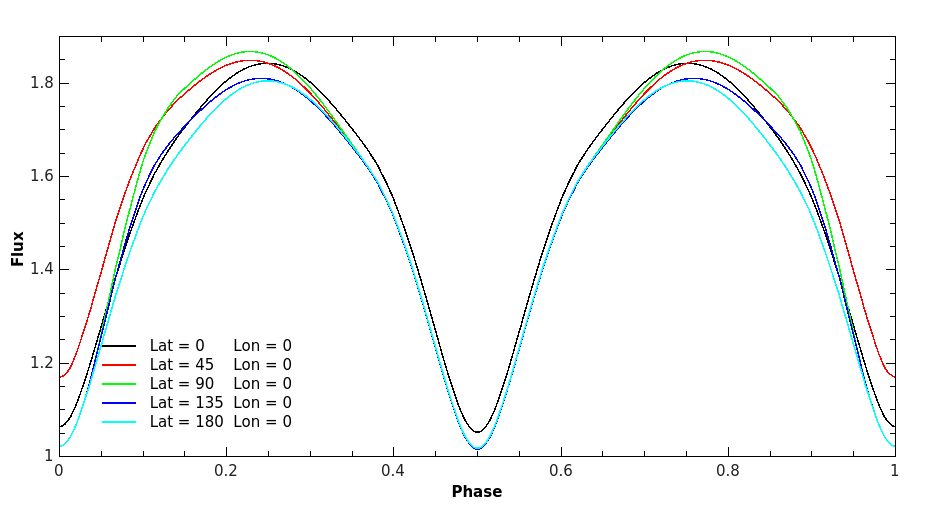
\includegraphics[width=\textwidth]{overc_spotT12_pos_lat.png}
        \caption{LC with spot on different colatitude and \\longitude = 0\degree}
    \end{subfigure}%
    \begin{subfigure}[t]{0.5\textwidth}
        \centering
        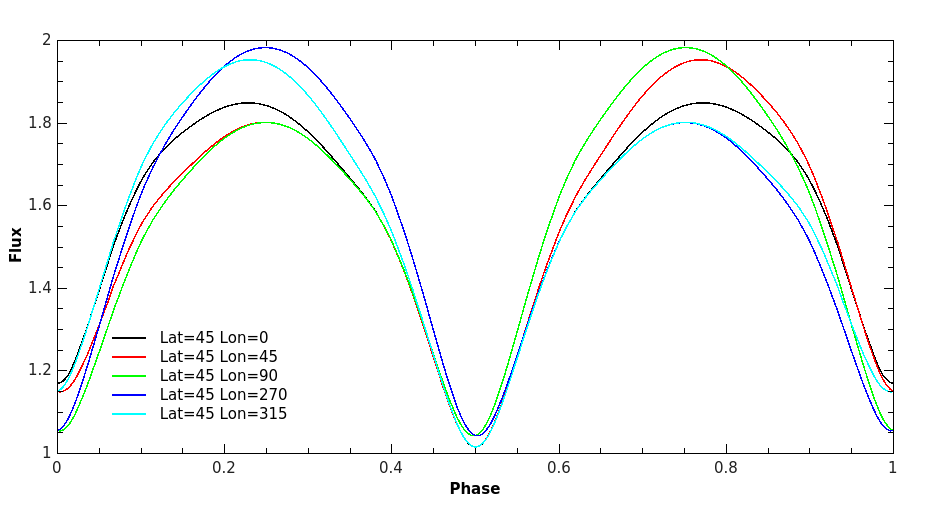
\includegraphics[width=\textwidth]{overc_spotT12_pos_lon.png}
        \caption{LC with spot on different longitude and \\colatitude = 45\degree}
    \end{subfigure}
    \caption{LC of contact binary system with "hot" spot ($T_{spot}=1.2~T_{surf}$) on primary component at different positions}
\label{fig:overcontact_spotT12_pos}
\end{figure}

%????
From previous results with detached EB system, we already know that smaller and colder spot adds more uncertainty to the definition of orbital elements of $3^{rd}$ body available in EB system. We can expect the same results with contact EB systems. 
So let us define an influence of the spot presence on primary and secondary EB components and spot migration. This two aspects can be often found in contact and overcontact systems.

For simulation of O-C diagram with two spots in EB system we locate the spot on secondary component at $lon=180\degree$, $colat=45\degree$ to make it visible to the observer. Radius of the spot on secondary component is $r_{spot_s}=35\degree$, temperature is $T_{spot_s}=0.8~T_{surf}$. The results of orbital parameters of $3^{rd}$ body determination for this case are presented in third column of table \ref{tab:3rd_body_overc_spot}.   

For simulation of O-C diagram with migrated spot over primary component of EB system we should define a parameters of the spot migration. 
According to \cite{Kalimeris2002} rotation period of starspot differs from $P_{eq}$ by:
\begin{equation}
\Delta P = P_\lambda-P_{eq},  % = \frac{P_{eq} \cdot k \cdot \sin^2\lambda}{1-k \cdot \sin^2 \lambda}
\end{equation} 
where $P_{eq}$ is the equatorial period of rotation ($P_{eq}=P_0$), and $P_{\lambda}$ is a period of starspot rotation equal to:

\begin{equation}
P_\lambda = P_{eq} \cdot (1-k \cdot \sin^{2}\lambda)^{-1}, 
\label{eq:Pl}
\end{equation} 

in equation \ref{eq:Pl} $k$ is a coefficient of differential rotation. For close binaries observation have indicated a range between 
$k\approx 6 \times10^{-4}$ and 0.18 with mean value $\bar{k}=3 \times10^{-2}$ \citep{Hall1990}. At the end of each orbital cycle, a starspot will shift  in longitude by: 
\begin{equation}
\delta \theta = 2\pi \frac{\Delta P}{P}
\end{equation}

If we calculate this value for our EB system with period $P=1.42834$ which has spot on latitude $\lambda=45\degree$ and mean value of $\bar{k}=3 \times10^{-2}$, we will get $\delta \theta = 5.4798\degree$ or $\delta \theta \sim 5.5\degree$. So spot with such parameters will do a full revolution in $\sim 65.5$ cycles or in our case this is equal to 93.5 days. To simplify the process of simulation we take an integer number of $\delta \theta = 6\degree$ in such case the spot will do a full revolution in 60 cycles or in 85.7 days. 

Large spots causing prominent light curve minima apparently can survive for many years, despite differential rotation, and form centres
of activity, or active longitudes \citep{Berdyugina2005}. Polar spots are found to have lifetimes of over a decade \citep{Hussain2002}.
Our simulation of $3^{rd}$ body is made on 5 years time interval so lets define that our spot lifetime is also 5 years.

Last question that we need to know is a radius of a spot. Lets consider a case with a spot radius $35\degree$ because a bigger spots are more typical for this type of EB systems. 

 
\begin{figure}[!h]
    \centering
    \begin{subfigure}[t]{0.5\textwidth}
        \centering
        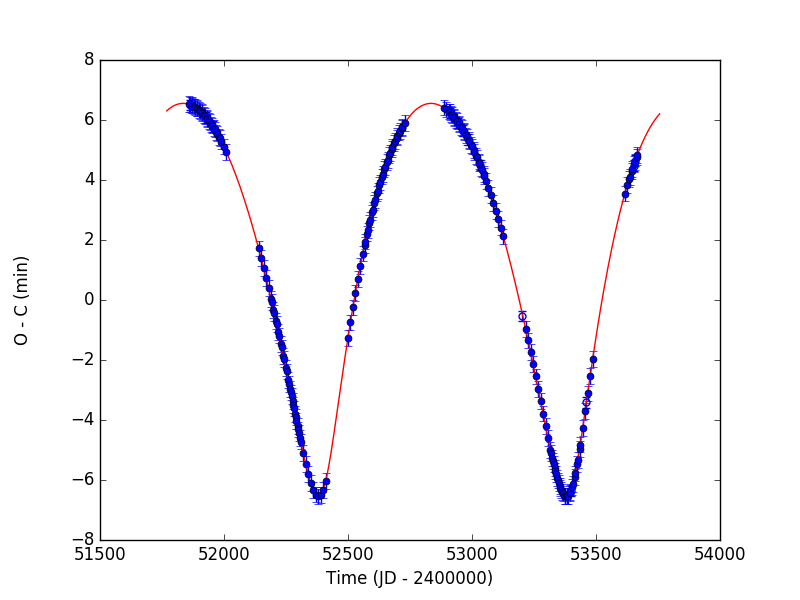
\includegraphics[width=\textwidth]{overc_ideal.png}
        \caption{o-c ideal}
    \end{subfigure}%
    \begin{subfigure}[t]{0.5\textwidth}
        \centering
        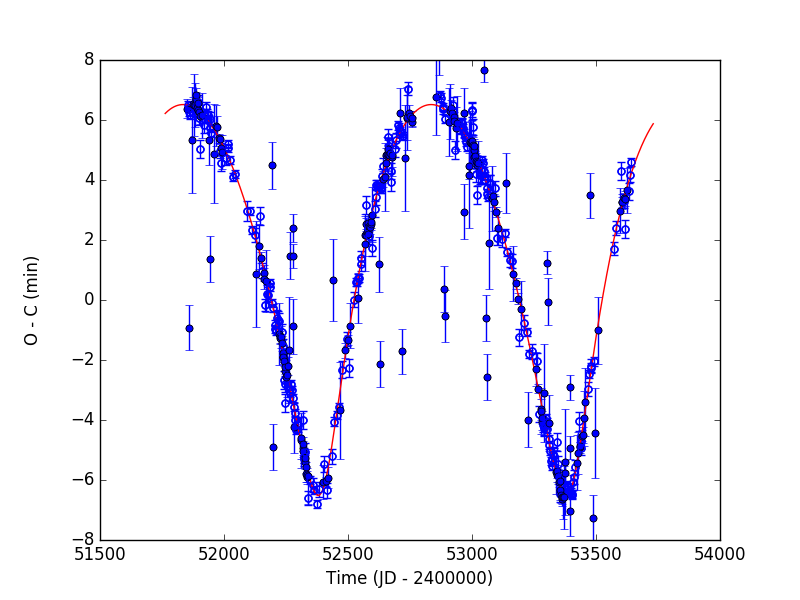
\includegraphics[width=\textwidth]{overc_spot_migr4.png}
        \caption{o-c with spot}
    \end{subfigure}
    \caption{O-C diagram for contact EB system with (b) and without (a) migrated spot.
        Red line - fit with MCMC method, correspond to values in table \ref{tab:3rd_body_overc_spot}. 
        Filled circles are primary minima, not filled circles - secondary minima.}
\label{fig:overcontact_spot_oc}
\end{figure}

From figure \ref{fig:overcontact_spot_oc} we can clearly see how migrated spot reduce precisions of minima exact time detection and in some cases, we even got point that does not fit in our O-C diagram. This means that these points are faults. Migrated spots are the most difficult cases for precise definition time of minima, make O-C diagram and define orbital parameters of $3^{rd}$ body.
Fitted parameters of orbit and $\chi^2$ values of fit are presented in table \ref{tab:3rd_body_overc_spot}. 
  
\begin{table}[!h]
 \caption{Orbital parameters of $3^{rd}$ body for contact EB system with two spots and migrated spot. Spot parameters $r_{spot}=35\degree$, $T_{spot}=0.8~T_{surf}$. For description of parameters see Table~\ref{tab:3rd_body_par}}
  \vspace{-6mm}
 \begin{center}
  \begin{tabular}{lcccc}
    \hline
    Solution            & Original       & no                  &   two        & migrated   \\
                        &                & spot                &   spots      & spot       \\
  \hline\noalign{\smallskip}                                                              
 $P$ [days]             & 1.42834        &           fixed     &   fixed      & fixed        \\ 
 $T_0$ [HJD]            & 2451852.3783   &           fixed     &   fixed      & fixed        \\
   \hline\noalign{\smallskip}                                                                                           
 $P_3$ [days]           &   1000         &          999.7(8)   &   999(1)     & 1000(1)      \\       
 $t_{03}$ [HJD]         & 2451400        &          2451400(2) &  2451402(2)  & 2451398(4)   \\
$a\sin i_3$ [AU]        &  0.797         &          0.799(3)   &  0.799(3)    & 0.764(3)     \\     
 $e_3$                  &  0.54          &          0.541(4)   &  0.532(5)    & 0.541(2)     \\            
$\omega_3$ [\degree]    &   288          &          288.1(7)   &  288.5(8)    & 287(1)       \\     
\hline\noalign{\smallskip}                                                                                         
$f(M_3)$  [M$_\odot$]   &  --            &          0.0681(8)  &  0.0683(9)   & 0.0666(7)    \\       
\hline\noalign{\smallskip}                                                                                  
$\chi^2$                &  --            &          0.614      &  6.547       & 2478.629      \\        
$\chi^2/n$              &  --            &          0.0283     &  0.0719      & 6.1200       \\       
\hline\noalign{\smallskip}  

\end{tabular}
\end{center}
\label{tab:3rd_body_overc_spot}
\vspace{-6mm}
\end{table}

\subsection{Pulsations in EB Systems}
Pulsation in eclipsing binary systems can be observed in Algol-type binaries, the so-called oEA stars (oscillating EA stars).
The oEA stars are mass-accreting main sequence A/F-type components in semidetached Algol-type eclipsing binary systems showing $\delta$~Sct - like pulsation \citep{Rodriguez2010}. The period of pulsation in such systems can vary from 20 to 300 minutes (see e.g \cite{Liakos2017}, \cite{Mkrtichian2007}). 

In work \cite{Liakos2017} relation for period of pulsation is given as:
\begin{equation}
P_{pul} = 0.031(4) + 0.009(1) P_{orb}. 
\end{equation} 

This relation is based on observation of $\delta$~Sct stars in all known close binaries systems (Detached, Semi-detached, unclassified). Coefficient of correlation for this relation is $r=0.62$.

To determine how the pulsations affect the O-C diagram and $3^{rd}$ precision of orbital elements we will consider three cases of detached EB systems with a different period of pulsations: 30, 150, 300 minutes.

To define the precise time of minima with pulsation presence it is very important to have a high rate of observation per some time interval (or per LC).
Until now we use synthetic LC generated by PHOEBE with sample rate 300 points per period. That was fully enough to precisely determine the time of the minima, but such rate is not enough for pulsations study.

To determine what sample rate should we use, let us check how the precision of primary minima is changed in detached EB system with added pulsations with parameters --- period $P_{pus}=30$ min and amplitude $A_{puls} = 0.02$. 
Three examples of same minima fitted in sample rates 300, 600 and 900 points per LC are presented on figure \ref{fig:puls_dif_rate}. If we have more than 900 points per LC then the precision of minima determination is slightly increasing to value 0.001 of a day. 
With the increase of sample rate, time of calculation also greatly increases, therefore the value of 900 points per LC is the best choice.

$3^{rd}$ body orbit parameters determined in detached EB system with pulsation with a period of 30, 150 and 300 minutes are presented in table \ref{tab:3rd_body_par_puls}. As we can see from a table, the most precise determination of orbit parameters corresponds to pulsation with the longest period. Vice versa most inaccurate parameters of orbit determination correspond to the shortest period. A short period of pulsations can't make it impossible to determine the precise time of minima, and as we show above it is also very important what resolution of LC do we have. 

\begin{figure}[!h]
    \centering
    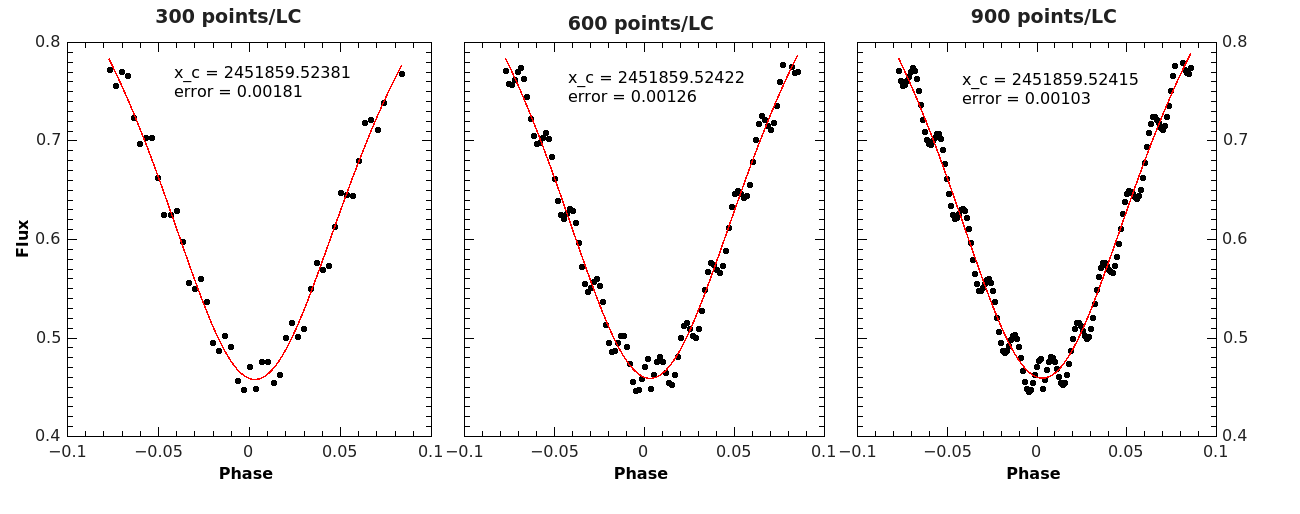
\includegraphics[width=\textwidth]{puls_dif_rate.png}
    \caption{Different sample rate and precision of primary minima determination. Black point are data from LC, red line - fitted minima.}
\label{fig:puls_dif_rate}
\end{figure}

%\begin{figure}[!h]
%    \centering
%    \begin{subfigure}[t]{0.325\textwidth}
%	    \centering
%	    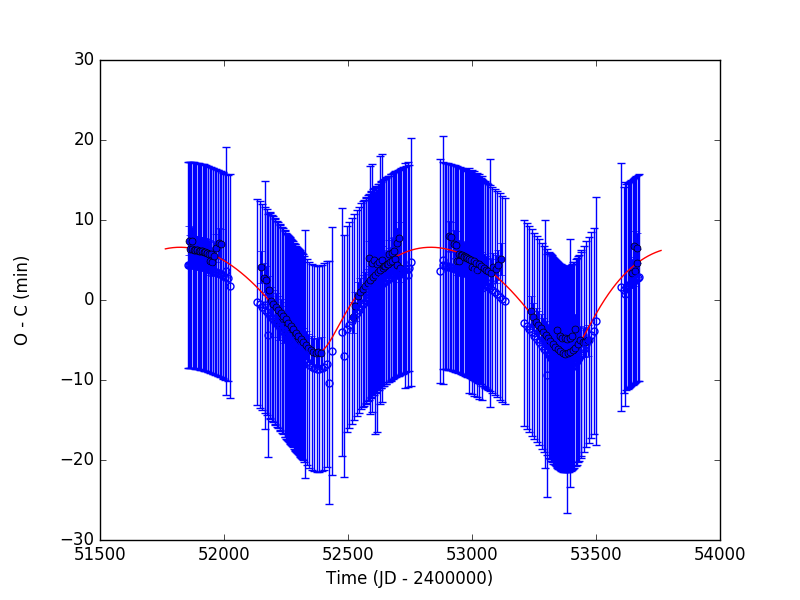
\includegraphics[width=\textwidth]{oc_puls_30m.png}
%%	    \caption{O-C diagram for 300 points/LC}
%    \end{subfigure}
%    \centering
%    \begin{subfigure}[t]{0.325\textwidth}
%	    \centering
%	    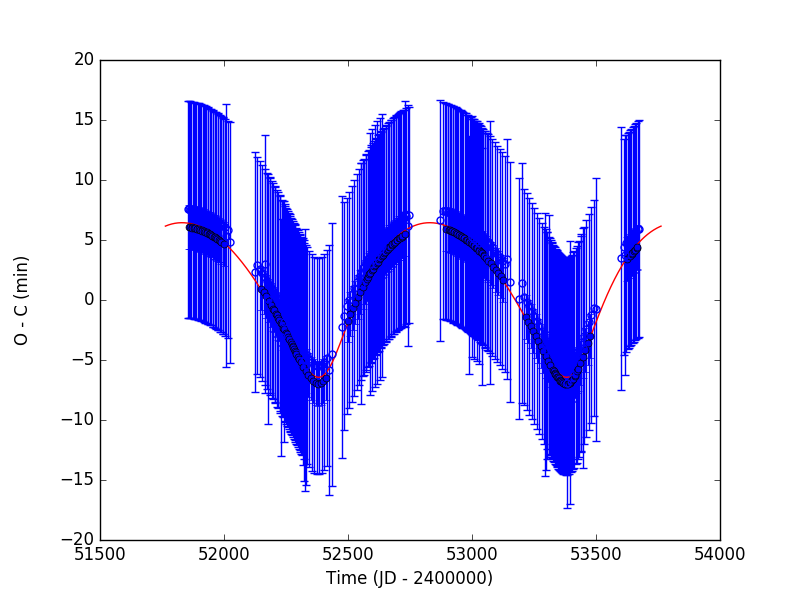
\includegraphics[width=\textwidth]{oc_puls_30m600.png}
%%	    \caption{O-C diagram for 600 points/LC}
%    \end{subfigure}
%    \centering
%    \begin{subfigure}[t]{0.325\textwidth}
%	    \centering
%	    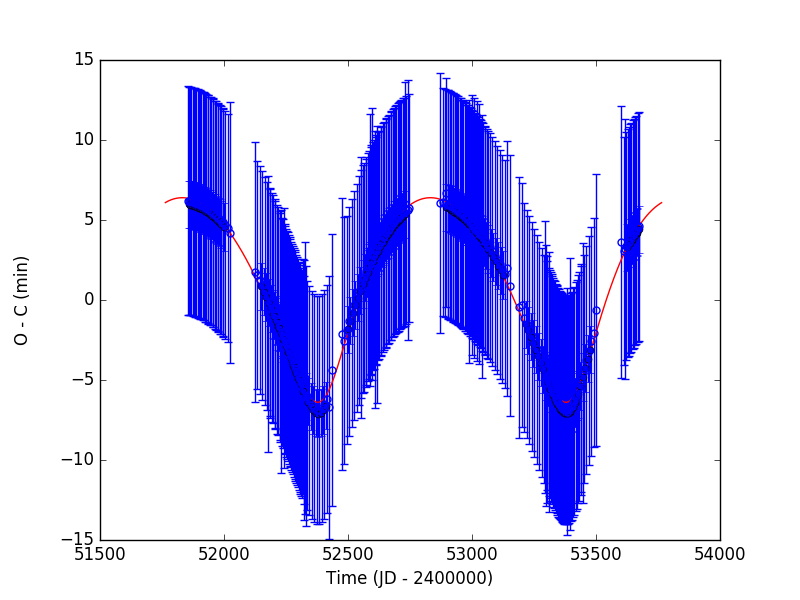
\includegraphics[width=\textwidth]{oc_puls_30m900.png}
%%	    \caption{O-C diagram for 900 points/LC}
%    \end{subfigure}
%    \caption{O-C diagrams with different sample rate. Left - O-C diagram for 300 points/LC, middle - for 600 points/LC, and right - for 900 points/LC}
%\label{fig:puls_dif_rate_oc}
%\end{figure}

\begin{table}[!h]
 \caption{Orbital parameters of $3^{rd}$ body for detached EB system with pulsations. 
 For description of parameters see Table~\ref{tab:3rd_body_par}}
  \vspace{-6mm}
 \begin{center}
  \begin{tabular}{lcccc}
    \hline
    Solution            & Original       & Pulsations         & Pulsations          & Pulsations \\
                        &                & $P_{puls}$=30 min  & $P_{puls}$=150 min  & $P_{puls}$=300 min\\
  \hline\noalign{\smallskip}                                                                                                                 
 $P$ [days]             & 1.42834        &           fixed     & fixed         & fixed        \\ 
 $T_0$ [HJD]            & 2451852.3783   &           fixed     & fixed         & fixed        \\
   \hline\noalign{\smallskip}                                                                             
 $P_3$ [days]           &   1000         &          1000(7)     & 1002(8)      &  1000(7)     \\       
 $t_{03}$ [HJD]         & 2451400        &          2451408(16) & 2451390(19)  &  2451399(19) \\
$a\sin i_3$ [AU]        &  0.797         &          0.778(19)   & 0.813(19)    &  0.807(19)   \\     
 $e_3$                  &  0.54          &          0.431(29)   & 0.600(28)    &  0.569(30)   \\            
$\omega_3$ [\degree]    &   288          &          291(5)      & 285(5)       &   288(5)     \\     
\hline\noalign{\smallskip}                                                                              
$f(M_3)$  [M$_\odot$]   &  --            &          0.0628(47)  & 0.0715(52)   &  0.0700(52)  \\       
\hline\noalign{\smallskip}                                                                          
$\chi^2$                &  --            &          8.519       & 2.778        &  0.802       \\        
$\chi^2/n$              &  --            &          0.0184      & 0.0069       &  0.0019      \\       
\hline\noalign{\smallskip}  

\end{tabular}
\end{center}
\label{tab:3rd_body_par_puls}
\vspace{-6mm}
\end{table}
\chapter{Circumbinary Planets and White Dwarfs in Kepler Eclipsing Binaries Catalog?}
\section{some text here}

\chapter{Conclusions}
Some conclusions.

% % % % %  To do LIST:
% + abstracti
%pridat intro na zaciatku . CH1 ?   
%+ outline
%pridat tabulu z BD  (exoplaneti) co su objavene v EB systemoch    V attach ked velke   (name, alfa, del, system, Mass, ref  )  NY Vyr ??
%
%Skusit urobit numeraciu obrazkov 1,2,3,4  a nie 1.1, 1.2,DONE,,,,,,,,,  +tabule?????

%Motivation .... outline ide na zaciatok.

%K O-C diagrams pridat obrazky O-C z mass transfer, applgate, 3rd body
% % % % % % %

%\chapter{O-C Diagrams}
\label{Chapter_oc}
\section{O-C Basics}
Observed minus Calculated diagrams is a diagnostic tool and involves the evaluation and interpretation 
of the disagreement between the measure of an observable event and its
predicted value \citep{Sterken2005basic}.
The idea that random processes may be important in determining O-C behaviour is not new, dating back at least to
\cite{Eddington1929}. Before dealing with the consequences for the statistics of
O-C diagrams, it is worthwhile to review possible physical causes of random
cycle-to-cycle period variations \citep{Koen2005stat}.

In astronomy, O-C usually implies a temporal aspect, and is used when
discussing cyclic phenomena where the times of occurrence of a given event is irregular. 
The O-C diagram is then constructed by plotting the quantity O-C as a function of time, the correct interpretation 
of these deviations leads to a better model (and a new O-C diagram).

In variable-star studies, O-C is sometimes expressed as deviations of phase
in the cycle of variability, whereas the time axis is the cycle number (commonly
indicated by $E$). In such studies, the O-C diagram mostly refers to rather
simple C formalisms, viz. linear or quadratic ephemeris formulae, sometimes
combined with a trigonometric periodic term \citep{Sterken2005basic}.

%Period of a recurrent phenomenon is the time interval after which the event 
%goes exactly through a same cycle again. In reality, we deal with cycles, rhythms, waves, and 
%pseudo-periods or characteristic times, in short, with processes that repeat themselves
%in a more or less regular way.

We are dealing with processes that repeat themselves in a more or less regular way.
Any attempt to construct a reliable O-C diagram will fail if a wrong
value of period $P$ is used. But it is not always easy to derive a period from the observational data: 
$P$ is not directly observable, it follows from the
determination of at least two moments of time of the same reference phase (epochs). 
The observation of two such epochs $T_{1}$ and $T_{2}$ immediately provide us an upper limit for $P$. 
When more than two such times are available, the period can be derived by a least-squares solution of a set of
equations
\begin{equation} \label{eq:period}
T_{i} - T_{j} = nP
\end{equation}
where $n$ is an integer, commonly called the cycle number $E$(epoch).

Phase is a position on the cycle of variation, a convenient periodic measure of
elapsed time: $\varphi (t)$ is the fraction of $P$ that elapsed since the occurrence of the
reference time $T_{0}$ and is given by

\begin{equation} \label{eq:phase}
\varphi = \frac{T-T_{0}}{P} ~\bmod~ 1
\end{equation}

The most common approach to the O-C procedure is the one in which one reference 
phase is selected, and where the timings of this reference phase are studied
and interpreted.
Several methods exist to determine the reference phase in a variability curve. 
This methods are discussed in Chapter \ref{Chapter_minima_det}.

\section{Constant and Variable Period}
If $P$ is constant and if its value is known, equation (\ref{eq:period}) leads to

%\begin{equation} \label{eq:Tmin}
%T_{max} = T_{0} + P E
%\end{equation}
%or,
\begin{equation} \label{eq:Tmin2}
T_{min} = T_{0} + P E
\end{equation}
where $T_{min}$ is the time of minimum light, $T_{0}$
is the zero epoch and $E$ is the number of cycles elapsed since the zero epoch. $T_{0}$ and
$P$ are obtained through a least-squares solution. The longer the time interval (in
cycles) over which the data have been collected, the higher will be the accuracy
of the solution for $P$: the uncertainty in $P$ is inversionally proportional to the
number of cycles, and proportional to the r.m.s. scatter of the data.

It is certainly not a trivial task to conclude from experimental data that a
significant period change has occurred. In principle, changes of period could
be described by any mathematical formula expressing $P$ as a function of time.
Thus, the time of epoch $T_{m}$ is

\begin{equation} \label{eq:P_var}
T_{m} = T_{0} + \int P(t)dt   ~~~~~\mathrm{or}~~~~~   T_{m} = T_{0} + \int P(E)dE
\end{equation}

In most cases, relation (\ref{eq:P_var}) is restricted to linear variations, cyclic variations, or
a combination of both of them.

Many causes can lead to period variations.
%the reference phase is seen systematically earlier (negative O-C) or later (positive O-C), 
%depending whether eclipsing variable is nearer or further from the observer. 
%Such meandering of the reference phase will result in a cyclic O-C diagram. 
%Apsidal motion in an elliptical orbit can re-orient the orbit with
%respect to the observer and cause an effect similar to the previous case. 
Transfer of matter (between stars in a multiple system) or mass ejection (from a system)
can provoke period changes. Periodic variations of O-C can indicate presents of other body in binary system.

If period changes linear with time, we will write $P$ as $P = a+bt$, where $t$ is the time, and $a,~b$ are constants.
Let $P_{0}$ be the period at $t=0$ and $\bar{P}$ is the average period over the whole time of observations, then

\begin{equation} \label{eq:P_lin_P}
P = a + b \bar{P}E
\end{equation} 
and
\begin{equation} \label{eq:P_lin_Pmid}
\bar{P} = a + \frac{1}{2}bt
\end{equation}  
so
\begin{equation} \label{eq:P_lin_Tm}
T_{m} = T_{0} + aE + \frac{1}{2}b \bar{P}E^{2}
\end{equation} 
with
\begin{equation} \label{eq:P_lin_add}
P_{0} = a,  ~~~~  \frac{dP}{dE} = b\bar{P},   ~~~~   \frac{dP}{dt} = b
\end{equation} 
expected time
\begin{equation} \label{eq:P_lin_Tm_res}
T_{m} = T_{0} + P_{0}E + \frac{1}{2} \frac{dP}{dt} \bar{P}E^{2}
\end{equation} 

\begin{equation} \label{eq:P_lin_OC_res}
O-C = \frac{1}{2} \frac{dP}{dt} \bar{P}E^{2}
\end{equation} 

%Equation (\ref{eq:P_lin_Tm}) is the most-frequently applied equation in O-C discussions. 
%Unfortunately, it is often misunderstood. Worse even, the factor $1/2$ is occasionally
%forgotten. The numerical value of $\frac{dP}{dt}$ is obtained through a quadratic fit, which
%also yields $P_{0}$.

When we now look at the O-C diagram for BW Vul in Fig.\ref{fig_oc}, we see that its
shape suggests a possible parabolic form, which seems to stand for a linear period
change. The least-squares parabolic fit to equation (\ref{eq:P_lin_Tm}) yields $P_{0} = 0.2010274$
and $\frac{dP}{dt}= 1.8 \cdot 10^{−10}$ days per cycle, or $~9.1 \cdot 10^{−10}$ day per day.

\begin{figure}[!ht]
\vspace{0cm}
\centerline{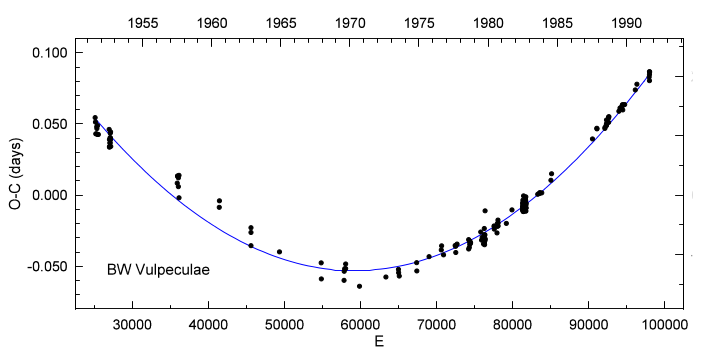
\includegraphics[width=0.65\textwidth]{oc_example.png}}
\caption{O-C diagram of some $T_{min}$ of BW Vul with best fit parabola. \citep{Sterken2005basic}}
\label{fig_oc}
\end{figure}

\begin{figure}[!ht]
\vspace{0cm}
\centerline{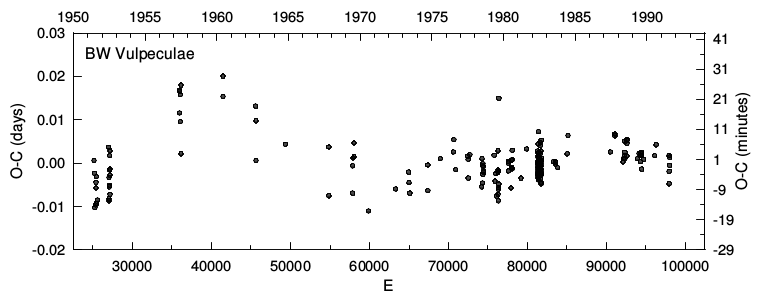
\includegraphics[width=0.65\textwidth]{oc_example_2.png}}
\caption{Differential O-C diagram after prewhitening with the fitted parabola. \citep{Sterken2005basic}}
\label{fig_oc2}
\end{figure}

When looking at Fig.\ref{fig_oc}, one notices that there are stretches of the O-C parabolic
fit where the data at one time are systematically above the fitted curve, and at
other times remain below the curve. Figure \ref{fig_oc2} shows the differences that were
obtained by removing the parabolic trend, and shows wave shape with
variable amplitude \citep{Sterken2005basic}. Such a trend, in particular when it repeats itself, 
can indicate presence of other body in binary system. 
In such case, O-C can be fitted with additional term corresponding to 3rd body orbit parameters:  

\begin{equation} \label{eq:P_lin_OC_sin}
T_{m} = T_{0} + P_{0}E + \frac{1}{2} \frac{dP}{dt} \bar{P}E^{2} +
\dfrac{a_{12}\sin i}{c}   \left[  \dfrac{1-e^2}{1+e \cos\nu}   \sin(\nu + \omega)  + e \sin \omega  \right]
\end{equation} 
 

%\begin{equation} \label{eq:P_lin_OC_sin}
%T_{m} = T_{0} + P_{0}E + \frac{1}{2} \frac{dP}{dt} \bar{P}E^{2} + A\sin(2\frac{\pi}{\Pi}E+\phi)
%\end{equation} 
%
%\begin{equation}\label{eq:4_mmm}
%T_{min} = JD_{0}+P \times E + Q \times E^2 + \dfrac{a_{12}\sin i}{c}   \left[  \dfrac{1-e^2}{1+e \cos\nu}   \sin(\nu + \omega)  + e \sin \omega  \right] 
%\end{equation}
where $a_{12} \sin i$ is the projected semi-major axis, $e$ is the eccentricity,
$\omega$ is the longitude of the periastron, $\nu$ is the true anomaly of the EB orbit around the common centre of the mass of
the whole system and $c$ is the velocity of light \citep{irwin1959}.

%\chapter{Minima Times Determination}
\label{Chapter_minima_det}
In order to obtain precise time of minima in eclipsing binary systems we need to define function that will fit minima shape with best precision.
There is to different approaches for eclipsing binary LC fit: (i) finding parameters of LC that will describe physical processes of binary star system or (ii) phenomenological (mathematical) modelling of observed data variations.

There is also a possibility to fit LC minima with simple functions or use Kwee and van Woerden method.
Individual approach requires narrow shape minima. Each branch of such minima must be fitted with some linear fit and time of minima will be found 
at the intersection of lines.

In this work we prefer to use phenomenological fitting methods or use simple function fitting, because we have a large number of eclipsing binary systems in Kepler EB catalogue. It is not possible to find each system's physical parameters in every case or it can take much longer time. All this methods are described below.


\section{Kwee and van Woerden Method}
Based on assumption that the set of data points around the minimum can be represented by the curve that is strictly 
symmetric with respect to the true minimum epoch $T_{0}$. Then an even function of time $\tau=T-T_{0}$ can be chosen to
fit the observations in sense of least-squares method. However the function itself is not evaluated. Instead a preliminary 
minimum time $T_{1}$ is estimated and $2K$ magnitudes (equation \ref{eq:kwee_m}) spaced at equal time intervals $\Delta$ symmetrically to $T_{1}$ are formed by linear interpolation between the observations.  Then $S(T_{1})$ is computed.
\begin{equation} \label{eq:kwee_m}
m_{\pm k} = m(T_{1}\pm k \Delta), ~~~ k=(1,K)
\end{equation}

\begin{equation} \label{eq:kwee_S}
S(T_{1}) = \sum_{k=1}^{K}(m_{k}-m_{-k})^2
\end{equation}

The procedure is repeated twice by shifting assumed minimum time by~ $\pm \Delta/2$ ~yielding $S(T_{1}+\Delta/2)$ ~and~ $S(T_{1}-\Delta/2)$.
The three values of $S$ define a parabola~ $S(T)=aT^2+bT+c$ ~with minimum at~ $T_{KW}=-b/2a$ ~which is considered to represent the 
true minimum time $T_{0}$. The mean error of minimum epoch is estimated by

\begin{equation} \label{eq:kwee_err}
\sigma_{KW} =\sqrt{\frac{4ac-b^2}{4a^2(Z-1)}} 
\end{equation}
where $Z$ is the number of independent magnitude pairs. For~ $2K=N$  ($N$ is a number of observations) the authors take  $Z=N/4$ ~if observations are not equally spaced in time ~\citep{kwee1956, brainhorst1973}.

Main disadvantage of this method is that we must have symmetrical shape of minimum and error of such method are unrealistically small. 

\section{Simple Function Methods}

\subsection{Fitting with Gauss and Lorentzian Functions}
The main advantage of this two functions is their simplicity and ability to get coordinates of centre ($x_{c}$) after fitting light curve.
With another more complex functions that are discussed below we must to derivate it before we can find $x_{c}$.

Gaussian function:
\begin{equation}\label{eq:gaus}
F(t)= A\cdot \exp(-\frac{(t - x_{c})^2}{2\sigma^2})
\end{equation}

Lorentzian function: 
\begin{equation}\label{eq:lorentz}
F(t)= A \frac{w^2}{w^2 + (t - x_{c})^2}
\end{equation}
where $A$ is the amplitude, $t$ is the time, $w$ is the half-width at half-maximum, $\sigma$ is the standard deviation and $x_{c}$ is the coordinates of centre. 

Functions perform good fit when EB minima has shape similar to normal distribution. In case of narrow minima such functions have a slightly larger error. Also, function perform good fit when we fit only minima part but not all light curve.

\subsection{Fitting with Polynomial Function}
Polynomial function is fitted to light curve in a time interval $2 \Delta t$, symmetric with respect
to the estimated minima time. The times of minima are then found using 
the calculated first derivatives, and the resulting list is processed again in
subsequent iterations. Two choices must be carefully made:
\begin{enumerate}
\item The optimal value of $\Delta t$: evidently, $\Delta t$ should comprise only those data
that contribute to the minimum event being considered, and should exclude 
data beyond the flection point. The time interval $\Delta t$ should by all
means be sufficiently large to avoid small-number statistics, and the fitted
parameters must be reasonably stable when omitting data points near the
edges of the interval $2 \Delta t$
\item The degree of the polynomial: parabolic fits are to be avoided, since they
force symmetry to the data. Polynomials of third degree work well if data
curves have a slight asymmetry, but for more extreme skewness, fourth- or
fifth-degree polynomials may be used. The order of the polynomial should
be appropriate in relation to the number of data points: though the formal
goodness of fit may appear to increase with increasing polynomial degree,
one should avoid high orders when dealing with sparse data.
\end{enumerate}

The choices are very much dictated by the data, perhaps most of all by the
observational precision, and by the time resolution.
The safest approach, probably, is to carry out a statistical investigation with a range of $\Delta t$ and polynomial
degrees 3-5 for every reference phase of every variable studied, and to select the
best-fit combination of reference phase, interval and polynomial degree for that
particular variable.

But the solution really depends on the chosen interval
and on the number of data, we should keep in mind the rule of thumb that the order
of the polynome should respect the number of fitted points \citep{Sterken2005basic}.

\section{Phenomenological Methods}
\label{phenom}
\input{phenom} 

\section{Template Method}
This method is based on assumptions described in \cite{Pribula2012, Pribulla2008}. 
%Another method is describer in \cite{Pribula2012, Pribulla2008}.
For each EB, the fitting templates $T(x)$ is prepared to obtain the time of minimum 
for any sufficiently long photometric sequence. In such way, not only the minima part of LC, but also other LC segments where
the brightness sufficiently changes can be used. The template LC can be produced as the average obtained over the whole 
available observations, or as a phenomenological model as mentioned in Section \ref{phenom}.

Due to the differences in filter transparencies and wavelength response of different used detectors, 
LC template must be formed for each filter separately and the fitting LC will be scaled to match the observations.
It is also noted that small nightly shifts effects of the LCs observed even with the same
instrument. Sometimes the LC shows slight but systematic slopes. These slopes are, very probably, caused by scattered
light combined with drifting of the targets on the CCD due to imperfect tracking of the telescope.
In order to obtain good fits of the template $T(x)$ to the observed LCs (and accurate timings), authors constructed the following
fitting function (see \cite{Pribulla2008}):

\begin{equation}\label{eq:dwarf1}
F(x) = A+Bx+CT(x-D)
\end{equation}
where $T(x)$ is a LC template, $A,B$ and $C$ describe shifting,
scaling and \textquote{slanting} of the LC template, and $D$ is shift in time to get exact time of minima. Fixing of the
parameters are judged according to the appearance of individual LCs.
%% Chapter 2
\chapter{Kepler Mission} % and data processing} % Main chapter title
\label{Chapter2} % For referencing the chapter elsewhere, use \ref{Chapter1} 

%----------------------------------------------------------------------------------------
% Define some commands to keep the formatting separated from the content 
%\newcommand{\keyword}[1]{\textbf{#1}}
%\newcommand{\tabhead}[1]{\textbf{#1}}
%\newcommand{\code}[1]{\texttt{#1}}
%\newcommand{\file}[1]{\texttt{\bfseries#1}}
%\newcommand{\option}[1]{\texttt{\itshape#1}}
%----------------------------------------------------------------------------------------

Kepler was launched into a trailing heliocentric orbit on March 7, 2009 UT. The Kepler Mission is
designed to detect transits of Earth-size planets in the “habitable zone” orbiting $9<m_{v}<15$, F through M
type dwarf stars by means of differential photometry of $\sim$100000 stars in the constellations Cygnus and
Lyra. The photometric precision is expected to be $20 ~ppm ~(\sim10^{-6} ~mag)$ for $12^{th}$ magnitude G2V stars, 
for a 6.5 hr integration. The sole scientific instrument is the Photometer, a 0.95 m aperture Schmidt telescope which
feeds the 94.6 million pixel CCD detector array, which contains both Science and Fine Guidance Sensor
(FGS) CCDs. The diameter of the FOV is 16.\degree1, of which 115.6 square degrees are covered with active
pixels
%. The area of active pixels vignetted by <11\% amounts to 101 square degrees. The four FGS CCD
%modules are mounted in the corners of the Science array to minimize thermomechanical drift between the
%attitude control system and the science CCDs, in order to attain the required~<0.009 arcsec $3\sigma$ 
%single-axis pointing stability 
\citep{kepler2009}.

The loss of two reaction wheels on the Kepler spacecraft has ended the primary mission data collection.
The Kepler project has proposed the K2 mission to NASA \citep{howel2014} that was approved on May 16, 2014.

\section{Kepler Data Characteristics}
A set of co-added and stored pixels obtained at a specific time is referred to as a cadence,
and the total amount of time over which the data in a cadence is co-added is the cadence
period. The two cadence periods in use are Long Cadence (LC) and Short Cadence (SC).
Each cadence consists of a series of frames that each include a 6.02 s exposure time and a
0.52 s readout time. For Long Cadence, 270 frames are co-added, for a total of 1766 s = 0.49~h. 
For Short Cadence, 9 frames are co-added, for a total of 58.85 s. Cadences are
absolutely and uniquely enumerated with cadence interval numbers (CIN), which
increment even when no cadences are being collected, such as during downlinks and safe
modes \citep{kepler2013}.

Data are time-stamped so that the mid-time of each cadence
is known with an accuracy of $\pm$ 0.050~s.

At the most basic level, it is important to understand that the
integrations underlying both SC and LC data are the same 6.02 s,
followed by the 0.52 s readout, before successive integrations
are summed into memory. There is no difference at which
saturation occurs for the 85.58 s cadence data versus the
29.42 minutes LC, since both are based on 6 s exposures.
Within the 58.85 s SC periods, 54.18 s is spent usefully
collecting photons while the remainder of the time is divided
between 9 readouts, which generates “smear” along the columns
as Kepler has no shutter \citep{gilliland2010}

Both cadences are stored on-board and downlinked to Earth roughly every 32 d, 
introducing gaps up to $\sim$24 h in length while the photometer is not collecting data.
Kepler completed one quarter of its orbit after three downlinks, and
must then perform a quarterly roll to keep its solar panels pointed
towards the Sun and its radiator pointed to deep space. Kepler data
are therefore organized into quarters and thirds around those rolls
and downlinks.

Pre-Q9, Kepler data were available in two forms: (i) 'raw' flux,
of which Simple Aperture Photometry (SAP) flux is the preferred
nomenclature, and for which basic calibration is performed distinguishing
it from the truly raw flux, and (ii) Pre-search Data
Conditioned (PDC) 'corrected' flux. The PDC data were created
as a step towards facilitating planetary transit searches and should
be used only with caution in astrophysical analyses because some
stellar variability can be modified in the light curves by the PDC
pipeline, pertaining to data releases 11 and earlier.
Post-Q9, PDC has been superseded by another pipeline, PDC MAP \citep{Murphy2012}. 
After July 2012 all quarters was reprocessed with pipeline and contain now PDC MAP flux.
On Figure \ref{fig_sclc} illustrated difference in data obtained in SC and LC mode. 

\begin{figure}[!t]
\vspace{0cm}
\centerline{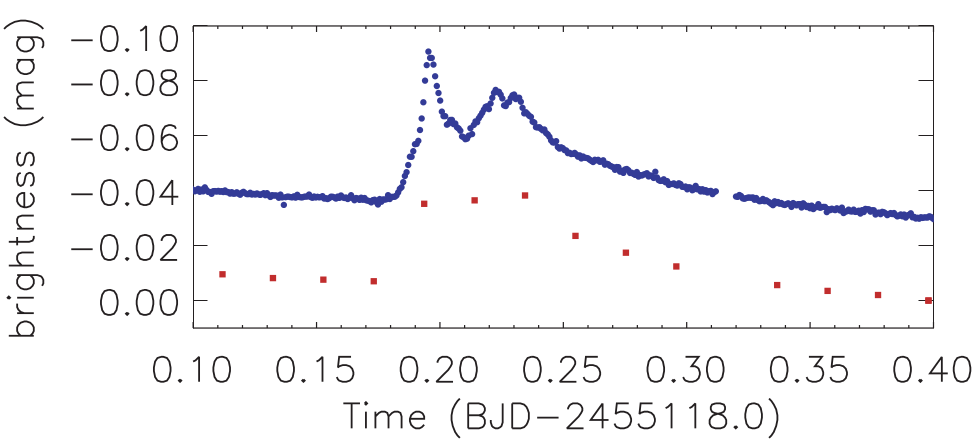
\includegraphics[width=0.80\textwidth]{sc_lc.png}}
\caption{A large-amplitude flare on KIC 12406908. The LC data (red squares) are 
plotted beneath the SC data (blue circles) for comparison. 
The change in brightness is precise, but not accurate – the dimmest LC point was
chosen as the zero-point for the graph, and all SC points are offset for clarity \citep{Murphy2012}.}
\label{fig_sclc}
\end{figure}

\section{Kepler Eclipsing Binary Catalog}

Large samples are useful to determine statistical properties
and for finding rare binaries which may hold physical significance (for example, binaries with very low mass stars,
binaries with stars in short-lived stages of evolution, very eccentric binaries that show large apsidal motion, etc.).
Catalogs of EBs from ground-based surveys suffer from various observational biases such as limited accuracy per
individual measurement, complex window functions (e.g., observations from ground based surveys can only be done
during nights with clear skies and during certain seasons).

The Kepler Eclipsing Binary Catalog lists the stellar parameters from the Kepler Input Catalog (KIC) augmented
by: primary and secondary eclipse depth, eclipse width, separation of eclipse, ephemeris, morphological classification
parameter, and principal parameters determined by geometric analysis of the phased light curve.
The online Catalog also provides the raw and detrended data for ∼30 minutes (long) cadence, and raw ∼1 minutes (short)
cadence data (when available), an analytic approximation via a polynomial chain, and eclipse timing variations. 

The construction of the Catalog consists of the following steps: 
\begin{itemize}[noitemsep]
\item EB signature detection; 
\item data detrending: all intrinsic variability and extrinsic variability are removed by the iterative 
fitting of the photometric baseline; 
\item the determination of the ephemeris: the time-space data are phase-folded and the dispersion minimized; 
\item Determination of ETVs;
\item analytic approximation: every light curve is fit by a polyfit; 
\item morphological classification via Locally Linear Embedding (LLE), a nonlinear dimensionality 
reduction tool is used to estimate the “detachedness” of the system;
\item EB characterization through geometric analysis;
\item diagnostic plot generation for false positive (FP) determination.
\end{itemize}


Only bonafide EBs and systems that clearly exhibit binarity through photometric analysis was accepted for inclusion in this catalog. 
Although best efforts have been taken to provide accurate results, there is caution that not all systems marked in the
Catalog are guaranteed to be EB systems. There remains the possibility that some grazing EB signals may belong to small
planet candidates or are contaminated by non-target EB signals. For now, 2878 objects are identified and analysed from the entire data set
of the primary Kepler mission (Q0-Q17) \citep{kirk2016}. In this work we are dealing with $3^{rd}$ release of this catalog.
%\chapter{Chances to Discover Circumbinary Object}
\label{Chapter3}

Chances to discover a circumbinary substellar body depend primarily on three factors: 
\begin{itemize}[noitemsep]
\item the precision and number of the minima which can be achieved;
\item the semi-amplitude of the LITE caused by the body;
\item the intrinsic variability of the binary causing noise in minima timings.
\end{itemize}
%(i) the precision and number of the minima which can be achieved;
%(ii) the semi-amplitude of the LITE caused by the body;
%(iii) the intrinsic variability of the binary causing noise in minima timings.

\section{Precision of the Minimum Time}
The precision of the minimum time $\Delta$t (for a triangular shape of the minimum) can be determined from equation (see, e.g., \cite{sybilski2010})

\begin{equation}\label{eq:dt}
\Delta t = \dfrac{D \sigma}{2d\sqrt{N}}
\end{equation}
where $\sigma$ is the brightness uncertainty (in magnitudes) of a single observational point, $D$ is the duration of the minimum, $d$ is the depth (in magnitudes) and $N$ is the number of observational points during the eclipse. 
The above relation shows that the precision of the minimum time increases with the number of data points taken in the minimum and their precision. The shape of the minimum also affects the precision of the timing -- deep and narrow minima provide the best precision.

In Table \ref{tb:lite_dt} calculated precision for 60 cm telescope of selected as example EB is presented, where $V$ is the out-of-eclipse brightness of the binary, $M_{1,2}$ -- masses of the component, $D$ -- duration of the primary eclipse, $d_{I}, d_{II}$ are the depths of primary and secondary minima, respectively, $\Delta T$ is the amplitude of the LITE for 1 Jupiter mass planet orbiting the binary on a 10 years orbit,
$\Delta t$ -- theoretically achievable primary minimum precision for a 60 cm telescope. 
On Fig.\ref{fig:4_depend} vertical black dash line is corresponding to the mean value of $\Delta t$ calculated for target list from \cite{Pribula2012},~ $\overline{\Delta t} = 2.8$ ~seconds.

\section{Amplitude of LITE Effect}
In case when an unseen third component revolves an EB, the residuals with respect to a linear (or quadratic) ephemeris will show
a wavelike behaviour in the O-C diagram because of the LITE.

The O-C curve (due only to the inner binary) can be described by a linear (constant period) or quadratic
ephemeris (linear period variation) and if a third body is orbiting the inner binary adding the LITE effect, the times
of the minima can be computed from equation (\ref{eq:P_lin_OC_sin}) from Chapter \ref{Chapter_oc}. 
%(a quadratic ephemeris added to the theoretical LITE given by formula (2) and (3) of \cite{irwin1959}).

%\begin{equation}\label{eq:4_minima}
%T_{min} = JD_{0}+P \times E + Q \times E^2 + \dfrac{a_{12}\sin i}{c}   \left[  \dfrac{1-e^2}{1+e \cos\nu}   \sin(\nu + \omega)  + e \sin \omega  \right] 
%\end{equation}

%where $a_{12} \sin i$ is the projected semi-major axis (inclination cannot be derived from the LITE alone), $e$ is the eccentricity,
%$\omega$ is the longitude of the periastron, $\nu$ is the true anomaly of the EB orbit around the common center of the mass of
%the whole system, $JD_{0} + P \times E + Q \times E^2$ is the quadratic ephemeris of the minima of the EB and $c$ is the velocity
%of light. The parameter $Q$ is the coefficient of the quadratic term and gives the rate of the orbital period change of the EB.

\begin{table}[!t]
 \centering
% \small
 \caption{Expected LITE amplitude for Jupiter-mass companion on 15-years orbit and theoretical precision for 60 cm telescope \citep{Pribula2012}.}
 \label{tb:lite_dt}
 \vspace*{1ex}
 \scalebox{1.0}{
 \begin{tabular}{c||c|c|c|c|c|c|c|c}\small
%   Star        &  V   & $M_{1}[M_{\odot}]$ & $M_{2}[M_{\odot}]$ &  $d_{1}[mag]$ & $d_{2}[mag]$ & $D[days]$ & $\Delta ~T[s]$ & $\Delta ~t[s]$ \\
   Star             &  V   & $M_{1}$       & $M_{2}$       &  $d_{I}$ & $d_{II}$ & $D$    & $\Delta T$ & $\Delta t$ \\
                    &  mag & $[M_{\odot}]$ & $[M_{\odot}]$ &  [mag]   & [mag]    & [days] & [s]         & [s] \\
\hline
DV Psc              & 10.6  & 0.49 & 0.51  &  0.32 & 0.15 & 0.062  & 4.5            & 1.1    \\
BX Tri              & 13.4  & 0.51 & 0.26  &  0.33 & 0.27 & 0.072  & 5.4            & 4.2     \\
V470 Cam            & 14.7  & 0.48 & 0.13  &  1.00 & 0.20 & 0.015  & 6.3            & 1.2     \\
GSC 19411746        & 12.9  & 0.56 & 0.65  &  0.90 & 0.40 & 0.453  & 5.1            & 6.1      \\
NY Vir              & 13.3  & 0.50 & 0.15  &  0.90 & 0.15 & 0.012  & 6.0            & 0.6   \\
NSVS 02502726       & 14.0  & 0.71 & 0.35  &  0.50 & 0.35 & 0.084  & 4.3            & 3.9    \\
NSVS 06507557       & 13.4  & 0.66 & 0.28  &  0.70 & 0.23 & 0.062  & 4.7            & 1.8    \\
MR Del              & 11.0  & 0.69 & 0.63  &  0.33 & 0.17 & 0.073  & 3.7            & 1.4      \\
\hline
 \end{tabular}}
\end{table}

The full amplitude of the expected LITE changes caused by another body orbiting a binary on the edge-on (i $\sim$ 90\degree ) circular orbit (e $\sim$ 0\degree) is:

\begin{equation}\label{eq:dT}
\Delta T = \dfrac{2M_{3}G^{1/3}}{c} \left[    \dfrac{P_{3}}{ 2 \pi \left( M_{1}+M_{2} \right) }   \right]^{2/3} 
\end{equation}
where $M_{1} , M_{2} , M_{3}$ are the masses of the components, $G$ is the gravitational constant, $c$ is the speed of light, 
and $P_{3}$ is the orbital period of the third (sub-stellar) component. Equation (\ref{eq:dT}) shows that the semi-amplitude of the LITE
changes is proportional to the mass of the third component and nearly proportional to its orbital period \citep{Pribula2012}. 
Amplitude of LITE effect depends on value of inclination $i$, so if it is less then $90\degree$, $\Delta T$ is decreasing too.   
Calculated value of $\Delta T$ for some binary systems is presented in Table \ref{tb:lite_dt}. 

Full amplitude of LITE effect from period of $3^{rd}$ body dependence is presented graphically on Fig.\ref{fig:4_depend}. %, \ref{fig:4_depend2}.

\begin{figure}[!ht]
\vspace{0cm}
\centerline{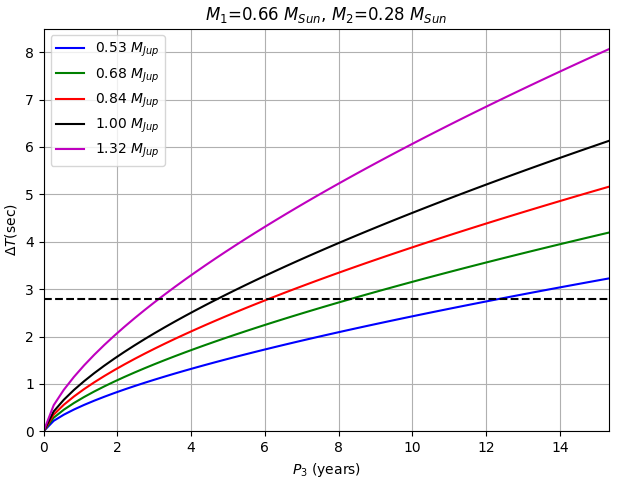
\includegraphics[width=0.8\textwidth,angle=0] {M3_dep_P_1.png}}
\centerline{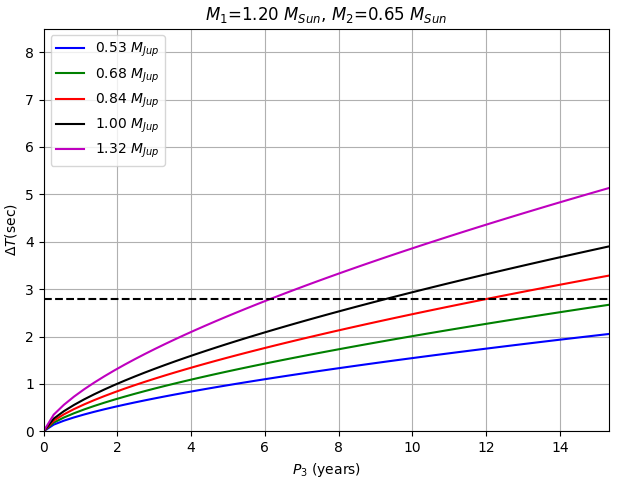
\includegraphics[width=0.8\textwidth,angle=0] {M3_dep_P_3.png}}
\caption{Amplitude of the expected LITE effect $\Delta T$ as the dependence of period of $3^{rd}$ body $P_{3}$. Different masses of third body $M_{3}$ in Jupiter masses is presented by different colours. Vertical dash line is a mean value of theoretical precision of minima $\Delta t$. 
Two graphs for different system components ($M_{1}, M_{2}$).}
\label{fig:4_depend}
\end{figure}

%\begin{figure}[!ht]
%\vspace{0cm}
%\centerline{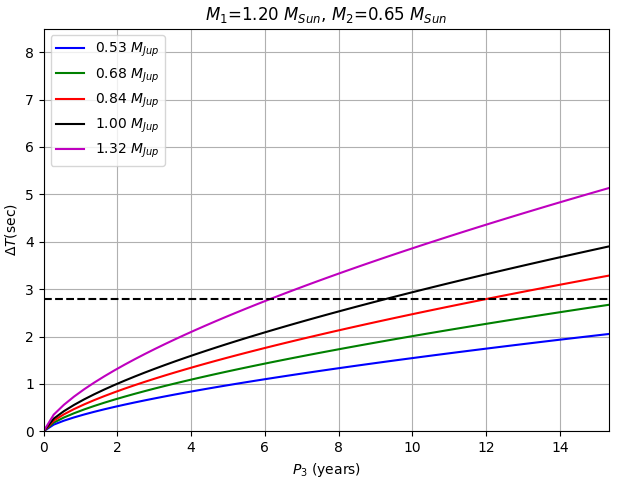
\includegraphics[width=0.8\textwidth,angle=0] {M3_dep_P_3.png}}
%\caption{Amplitude of the expected LITE effect $\Delta T$ as the dependence of period of third body $P_{3}$.  Different masses of third body $M_{3}$ in Jupiter masses is presented by different colours. Vertical dash line is a mean value of theoretical precision of minima $\Delta t$.}
%\label{fig:4_depend2}
%\end{figure}

As can be seen from graphs, minimum amplitude from LITE that can be registered by ~$\sim$ half meter telescope corresponds to one Jupiter mass body or force us to observe binary system on very long time intervals (>15 year). Otherwise, in case of Kepler EB catalogue we have magnitude precision $10^{-6}$, larger diameter, brightness uncertainty $\sigma$ and sometimes more points on minima, that can decrease value of theoretical minima precision $\Delta t$ and allow us to define exoplanets or brown dwarfs in eclipsing binary systems with masses of third body less then one Jupiter mass.  

\section{Building O-C Diagrams from Kepler Data}
Kepler satellite provides us with unprecedented accuracy of photometric data.
Such a huge database of EBs observed with high precision and monitored continuously over a period of several years
encouraged several teams to look for a periodic modulation of data, indicative of multiple systems.  
For example, \cite{gies2012} presented 41 suspected triples, while \cite{conroy2014} listed 236
potential triples. Moreover, \cite{Rappaport2013} presented 39 dynamically interesting systems, where
the third-body periods are short enough (if compared with the binary period) that some interaction between the orbits is
expected or even observed (e.g., changing of the inclination).
On the other hand, most of the triples listed in \cite{conroy2014} have periods of the order of hundreds or even thousands
of days, so long periods were usually only estimated (due to limited coverage of the Kepler data) or were influenced by
large errors \citep{Zasche2015}.

For this reason, we decided to perform a similar analysis to detect circumbinary objects for other systems, but based on a
larger data set if available, and taking into account different phenomena that distort EBs light curve.

In order to define the time of minima from available light curve in Kepler EB catalogue, special python script was written. 
This algorithm reads Kepler input catalog ID (KIC), period and initial epoch of binary system from Kepler EB catalogue. According to obtained KIC, we check if ~short or long cadence data, or both of them, are available, and start to process this light data.

In order to find the exact time of minima different methods can be used, most popular of them are described in Chapter \ref{Chapter_minima_det}. In this preliminary analysis we use fitting with Lorentz function (see equation \ref{eq:lorentz}) because it is simple method with good accuracy. In dissertation thesis we plan to compare mentioned methods and the best one will be used. Using Lorentz function we do not fit whole light curve, only the minimum part, for primary minimum we use only data with phase in range $-0.25 < \varphi < 0.25$.

Also, we can cut upper part of LC, for example taking into account only 70\%~-~90\% of LC amplitude, such approach increase fit precision. This is demonstrated on Fig.\ref{fig:ind_min_fit},\ref{fig:ind_min_fit2}. The only warning, in such approach, is to get enough data points because, as we know, precision of minima also depends on number of used points. 
\begin{figure}[!t]
\vspace{0cm}
\begin{tabular}{ll}
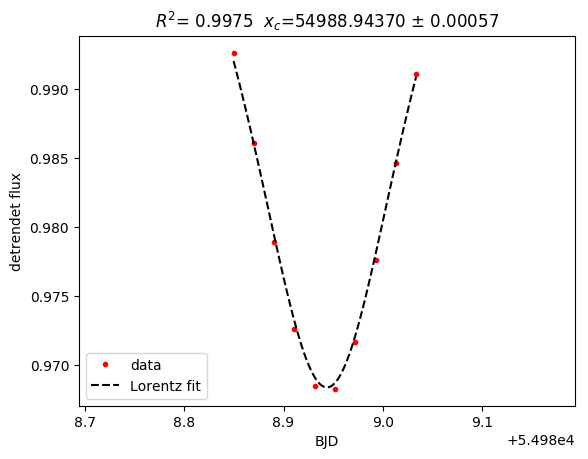
\includegraphics[width=.49\textwidth,angle=0] {lor/54988_9437025_08.png}
&
\includegraphics[width=.49\textwidth,angle=0] {lor/54988_9445532_1.png}
\end{tabular}
\caption{Individual minima fit (dashed line) of KIC 4681152 primary minima. Same minima fitted on two figures. Left: 80\% of amplitude Right: 100\% of amplitude}
\label{fig:ind_min_fit}
\end{figure}
\begin{figure}[!t]
\vspace{0cm}
\begin{tabular}{ll}
\includegraphics[width=.49\textwidth,angle=0] {lor/2/85_56164_3332913.png}
&
\includegraphics[width=.49\textwidth,angle=0] {lor/2/100_56164_3332725.png}
\end{tabular}
\caption{Individual minima fit (dashed line) of KIC 12553806 primary minima. Same minima fitted on two figures. Left: 85\% of amplitude Right: 100\% of amplitude}
\label{fig:ind_min_fit2}
\end{figure}

On the final stage, new ephemeris is computed and O-C diagram is formed from obtained times of minima. Some of these O-C diagrams are presented on Fig.\ref{fig:oc}. Having precessed, in such way, all binary systems in Kepler EB catalogue we have highlighted, in a first approximation, 169 systems with possible circumbinary objects or other physical phenomenons that are appearing on O-C diagrams. Some of these binary systems are highlighted for sure, and in many cases good detected systems are marked as multiple previously in works of ~\cite{gies2012, Rappaport2013, conroy2014}. There is also lot of candidates which will be studied more accurately with considering of other factors influence.   
\begin{figure}[!th] 
  \begin{subfigure}[b]{0.5\linewidth}
    \centering
    \includegraphics[width=0.95\linewidth]{oc/oc_8719897.png} 
    \caption{O-C diagram of KIC 8719897.} 
    \label{fig:oc:a} 
    \vspace{4ex}
  \end{subfigure}%% 
  \begin{subfigure}[b]{0.5\linewidth}
    \centering
    \includegraphics[width=0.95\linewidth]{oc/oc_9912977.png} 
    \caption{O-C diagram of KIC 9912977.} 
    \label{fig:oc:b} 
    \vspace{4ex}
  \end{subfigure} 
  \begin{subfigure}[b]{0.5\linewidth}
    \centering
    \includegraphics[width=0.95\linewidth]{oc/oc_8043961.png} 
    \caption{O-C diagram of KIC 8043961.} 
    \label{fig:oc:c} 
  \end{subfigure}%%
  \begin{subfigure}[b]{0.5\linewidth}
    \centering
    \includegraphics[width=0.95\linewidth]{oc/oc_10226388.png} 
    \caption{O-C diagram of KIC 10226388.} 
    \label{fig:oc:d} 
  \end{subfigure} 
  \caption{Illustration of few obtained O-C diagram with possible presence of 3rd body}
  \label{fig:oc} 
\end{figure}
%\chapter{Future Plans for Dissertation Thesis} % Main chapter title
\label{Chapter_Aim} % For referencing the chapter elsewhere, use \ref{Chapter1} 

%----------------------------------------------------------------------------------------

% Define some commands to keep the formatting separated from the content 
%\newcommand{\keyword}[2]{\textbf{#1}}
%\newcommand{\tabhead}[2]{\textbf{#1}}
%\newcommand{\code}[2]{\texttt{#1}}
%\newcommand{\file}[2]{\texttt{\bfseries#1}}
%\newcommand{\option}[2]{\texttt{\itshape#1}}

%----------------------------------------------------------------------------------------

In the dissertation thesis we plan to study circumbinary objects discovered in EB systems. 

The particular objectives of our research are specified in the following:

\begin{enumerate}

\item We will analyse Kepler data available in public archive.
\item We will also study influence of intrinsic variability of components and spots on the resulting O-C diagram.  
\item We will determine minima light of EB from Kepler and construct O-C diagram. Based on the shape of O-C diagram decision regarding presents of
another body in the system will be made. 
\item Parameters of other bodies in selected systems will be calculated.  


\end{enumerate}
%----------------------------------------------------------------------------------------
%	THESIS CONTENT - APPENDICES
%----------------------------------------------------------------------------------------

%\appendix % Cue to tell LaTeX that the following "chapters" are Appendices

% Include the appendices of the thesis as separate files from the Appendices folder
% Uncomment the lines as you write the Appendices



%----------------------------------------------------------------------------------------
%	BIBLIOGRAPHY
%----------------------------------------------------------------------------------------

%\printbibliography[heading=bibintoc,title={References}]

%\setlength\bibitemsep{10pt}
%\setlength{\bibsep}{0pt}
\setlength{\bibsep}{0pt plus 0.3ex}
%\setstretch{1}
\bibliography{biblio_lib}

%----------------------------------------------------------------------------------------


%\includepdf[pages=-]{Appendices/aasp-kudak-OC.pdf}
%\begin{appendices}
%
%\end{appendices}

\end{document}
